% \documentclass[man]{apa7}
\documentclass[stu]{apa7}

\usepackage{lipsum}

\usepackage[american]{babel}
\usepackage{multirow}
\usepackage{bm}
\usepackage{float}
\usepackage{subcaption}
\usepackage{amsmath}
\usepackage{nicematrix}
\usepackage{longtable}
\usepackage{fancyvrb}
\usepackage{listings}
\usepackage{lineno}
\usepackage{ragged2e}
\usepackage{graphicx}
\usepackage{pgfplots}
\pgfplotsset{compat=1.18}
\usepackage{hyperref}

\usepackage[dvipsnames]{xcolor}
\usepackage{tikz}
\colorlet{reviewColour}{blue}

\usepackage[figuresright]{rotating}

\newcommand*{\Scale}[2][4]{\scalebox{#1}{$#2$}}%
\renewcommand{\raggedright}{\justifying}

\usepackage{csquotes}
\usepackage[style=apa,sortcites=true,sorting=nyt,backend=biber,uniquename=false]{biblatex}
\DeclareLanguageMapping{american}{american-apa}
\addbibresource{references.bib}
% \DeclareLanguageMapping{english}{english-apa}
% \linenumbers

% \renewcommand{\raggedright}{\iustifying}

\hypersetup{
  colorlinks=true,
  linkcolor=blue,
  urlcolor=blue,
  citecolor=blue,
}

% Beyond Continuous Outcomes: 
% Disaggregation Under Dichotomies: Retrieving Within-Person Effects with Binary Predictors and Outcomes 
% Retrieving within-person effects
% Modeling Frameworks and Variable Types
% Binary Predictors and Outcomes in Multilevel Modeling: Understanding Within and Contextual Effects

% Within- and Between-Person Effects in Longitudinal Data: Comparing MLM and GEE Across Continuous and Binary Variables 
% 1. Within- and Between-Person Effects in Longitudinal Data: Moving Beyond Continuous Variables and the MLM to Binary Variables and GEE.
% % 2. Multilevel Models and Generalized Estimating Equations in Longitudinal Research: Extending Disaggregation to Binary Data
% 3. Multilevel Models and Generalized Estimating Equations: Retrieving Within-Person Effects in Binary Clustered Longitudinal Data.
% 4. From MLM to GEE: Revisiting Within- and Between-Person Effects with Binary Predictors and Outcomes.

\title{From Multilevel Modeling to GEE: Revisiting the Within- and Between-Person Debate with Binary Predictors and Outcomes}
\shorttitle{WITHIN-PERSON EFFECTS AND BINARY VARIABLES}

\author{\textbf{Ward B. Eiling (s9294163)} \vspace{1cm}}
\authorsaffiliations{Department of Methodology and Statistics, Faculty of Social and Behavioural Sciences, Utrecht University \vspace{1cm}}
\course{}
\professor{prof. dr. Ellen Hamaker \& dr. Jeroen Mulder \vspace{1cm}}
\duedate{\today \vspace{1cm}}
\note{Word count: 9,267/12,000 \\ FETC-approved: 24-2003 \\ \vspace{1cm} \textit{Candidate Journal: Psychological Methods}}

% \leftheader{Eiling}

% Abstract (max 250 Words (233 words now))
\abstract{\justify In longitudinal studies with clustered data, researchers are often interested in estimating within-person effects—how changes over time within one variable relate to changes in another. To properly isolate these effects, the multilevel linear modeling (MLM) literature has long emphasized the need to disentangle within- and between-person effects, typically using disaggregation techniques such as person-mean centering. However, these methods have been developed primarily for continuous predictors and outcomes and little attention has been paid to their application with binary predictors or outcomes, despite the prevalence of such variables in applied research. Moreover, the capacity of alternative estimation frameworks, such as Generalized Estimating Equations (GEEs), to recover these effects remains underexplored. This study addresses both gaps. First, we explain how within- and between-person effects may be understood for binary predictors and outcomes using four generative models. Second, we evaluate the performance of disaggregation methods across estimation frameworks (multilevel models vs. GEE) and predictor and outcome types (binary vs. continuous) in retrieving within-person and contextual effects. Our results indicate that both Mundlak’s contextual and hybrid approaches generalize robustly across all multilevel specifications. Person-mean centering—often considered the gold standard—performs similarly with continuous outcomes but is less effective with binary outcomes. GEEs implemented with disaggregation methods are able to recover effects when outcomes are continuous, but not when they are binary. We conclude with practical recommendations for model specification and offer directions for future research. 
}

% \abstract{\justify In clustered longitudinal data, a fundamental methodological concern is the \textit{contextual effect}: the possibility that the relationship between a predictor and outcome differs at the within- and between-person level. The multilevel linear modeling (MLM) literature offers established methods—such as person-mean centering—that dissaggregate  within-person and contextual components in the context of continuous predictors. However, limited attention has been paid to how such strategies generalize to binary predictors and outcomes, despite their ubiquity in applied research. Furthermore, alternative estimation frameworks such as Generalized Estimating Equations (GEEs) are commonly used in biostatistics, yet their capacity to recover within-person and contextual effects remains underexplored in this context. This study addresses this gap by systematically evaluating the performance of disaggregation methods across multilevel models and GEEs, focusing particularly on binary predictors and outcomes. We formalize four generative models to conceptualize within- and between-person effects across variable types, and conduct a simulation study that varies sample size, disaggregation strategy, predictor and outcome type, and modeling framework. Results reveal that Mundlak's contextual method generalizes well to all examined multilevel model, whereas person-mean centering yielded biased estimates under binary outcomes due to the non-linearity of the logit link. Disaggregation strategies proved viable in GEEs with continuous outcomes, where it performed comparably well for continuous outcomes, but yielded consistently different estimates under binary outcomes. We provide practical recommendations to improve model specification and interpretation in applied settings, aiming to bridge methodological gaps in the analysis of clustered binary data.}

% \abstract{Disentangling within- and between-person effects is critical for causal inference in longitudinal research with clustered data. While multilevel modeling (MLM) offers established strategies—such as person-mean centering—to estimate contextual effects with continuous predictors, methodological guidance is limited for binary predictors and outcomes. This poses challenges in psychological research, where binary variables are common, and risks misinterpretation in generalized linear multilevel models (GLMMs) due to nonlinearity in the link function. Generalized Estimating Equations (GEEs), frequently used in biostatistics, offer an alternative with distinct assumptions and estimation properties, yet their capacity to recover within-person and contextual effects remains underexplored in this context. We present a comprehensive simulation study evaluating estimation performance across GLMM and GEEs for different predictor and outcome types (binary vs. continuous), variable inclusion strategies (e.g., Mundlak’s contextual model), and sample sizes. Results reveal that GLMMs generalize well to binary settings and highlight critical limitations in interpreting GEEs estimates under non-continuous outcomes. We provide practical recommendations to improve model specification and interpretation in applied settings, aiming to bridge methodological gaps in the analysis of clustered binary data.}

% Keywords (Up to five keywords or brief phrases)
\keywords{clustered longitudinal data, contextual effect, person-mean centering, generalized estimating equations, multilevel models}

% \authornote{
%    \addORCIDlink{Ward B. Eiling}{0009-0007-8114-9497}
%   Correspondence concerning this article should be addressed to Daniel A. Weiss, Department of Educational Psychology, Counseling and
%   Special Education, A University Somewhere, 123 Main St., Oneonta, NY
%   13820.  E-mail: daniel.weiss.led@gmail.com}

\begin{document}

\maketitle

% Start the manuscript

% \subsection{Paragraph 1: Set the stage}

Across a wide range of disciplines, researchers analyze clustered longitudinal data to investigate prospective---and potentially causal---relationships between variables. When analyzing such data, psychological researchers commonly use the multilevel linear modeling (MLM) framework \parencite[]{bauer_fitting_2011}. A fundamental concern within the MLM literature is that the relationship between a predictor and an outcome may differ across levels of analysis \parencite[e.g.,][]{enders_centering_2007, kreft_effect_1995, raudenbush_hierarchical_2002}. In the context of longitudinal data, this implies that relationships across time captured at the within-person level of a model may differ from stable, between-person relationships as captured at the between-person level of a model. This discrepancy, known as the \textit{contextual effect}, is particularly important because failing to account for it results in an ``uninterpretable blend'' of within- and between-cluster relationships \parencite[139]{raudenbush_hierarchical_2002}. This blending obscures the within-person effect, which is typically the primary target of inference.

% \subsection{Paragraph 2: Build up the tension}

The MLM literature offers several \textit{disaggregation methods} that disentangle within-person from between-person effects \parencite[]{curran_disaggregation_2011}. These include: (a) person-mean centering of predictor variables; and (b) entering uncentered predictors alongside cluster means as predictor of the random intercept \parencite[]{kreft_effect_1995, raudenbush_hierarchical_2002, bell_explaining_2015}. However, the MLM literature has primarily focused on continuous predictors, with limited guidance on how to disentangle effects when dealing with \textit{binary predictors}. As a result, applied researchers may default to intuition or omit centering altogether when analyzing categorical predictors \parencite[]{yaremych_centering_2023}. This issue is exacerbated in generalized linear mixed modeling (GLMM)\footnote{We refer to GLMM as the general estimation framework that includes MLMs for continuous outcomes and multilevel logistic models for binary outcomes.} with \textit{binary outcomes}, where the non-linearity between predictor and outcome further complicates interpretation \parencite[]{austin_intermediate_2017, bolger_intensive_2013}. This gap in methodological guidance is concerning since binary variables are ubiquitous within the social sciences and researchers may be left unsure of how to specify their models correctly. 

% \subsection{Paragraph 3: Build up the tension even more}

A well established alternative for analyzing clustered data is the Generalized Estimating Equations (GEEs) framework. It was originally developed in the biostatistics literature to accommodate longitudinal designs with non-normal outcomes \parencite[]{liang_longitudinal_1986, zeger_longitudinal_1986}. In biomedical studies, GEEs is widely used—and often favored over GLMMs—for modeling binary outcomes \parencite[cf.][]{diggle_analysis_2002}. An important strength of GEEs is its reliance on fewer unverifiable assumptions compared to GLMM \parencite[]{mcneish_unnecessary_2017, hubbard_gee_2010}. As GEEs gains traction in psychology \parencite[e.g.,][]{mcneish_unnecessary_2017, muth_alternative_2016}, researchers familiar with MLM may question how GEEs compares to GLMMs and specifically whether the debate about separating within- from between-person effects using disaggregation method also applies when a GEEs approach is taken. While some prior work has addressed how to handle binary predictors in MLMs \parencite{yaremych_centering_2023, enders_centering_2007, raudenbush_hierarchical_2002} or binary outcomes in GLMMs \parencite{bolger_intensive_2013, schunck_within-_2017}, and others have compared estimation frameworks across disciplines \parencite{mcneish_unnecessary_2017, ballinger_using_2004, yan_comparing_2013, muth_alternative_2016, neuhaus_comparison_1991}, no study to date has examined how different disaggregation methods perform and compare across estimation frameworks and variable types. 

% \subsection{Paragraph 4: Aim of the Current Study (potential resolve?) and outline }

This paper seeks to address this gap by offering a systematic comparison of disaggregation methods across estimation frameworks and data types. Specifically, the goal of this paper is twofold. First, we aim to clarify how we should think about within and between effects with a binary predictor and/or outcome. Second, we study the degree to which we can correctly estimate these effects with GLMM and GEEs implementations. This article is structured as follows. We outline four data generating models to conceptualize within-person and contextual effects across different measurement scales, supported by a running example. Next, we discuss estimation frameworks and methods for including predictors. We then present a simulation study in which we assess estimation performance across variations in (a) estimation strategy (GLMM vs. GEEs), (b) disaggregation methods, (c) measurement levels (binary vs. continuous), and (d) sample size---number of clusters and number of measurements per cluster. We evaluate when common modeling choices may lead to biased estimates and provide practical guidance for applied researchers working with clustered binary data. We conclude with a summary of key findings, limitations, and directions for future research. 

\section{Data Generating Models}

In this section, we describe the four data generating models (DGMs) used to investigate contextual as well as within- and between-person effects in the context of binary predictors and/or outcomes. These models also form the basis of the simulation study. The DGMs differ in the measurement level of the predictor $X$ and the outcome $Y$, and are visualized in Figure~\ref{fig:path}. In all four DGMs, we consider a single time-varying predictor $X$, which reflects both stable between-person differences and within-person variation over time. Similarly, $Y$ is a time-varying outcome that exhibits both between-person differences and within-person fluctuations. $Y$ is affected by $X$ at both levels. For a given individual, a time-point-specific increase in \( X \) leads to a change in \( Y \), which we refer to as the within-person effect. Additionally, individuals with higher person-level averages of \( X \) obtain systematically greater changes in \( Y \) than predicted by the within-person effect alone, suggesting a contextual spill-over effect.

\newpage
\begin{center}
    \captionof{figure}{Path diagrams of Generative Models with Within-Person ($\beta_1$) and Contextual Effect ($\gamma_{01}$)}
    % Top row
    \begin{minipage}[t]{.49\linewidth}
        \centering
        \begin{subfigure}[b]{\linewidth}
            \centering
            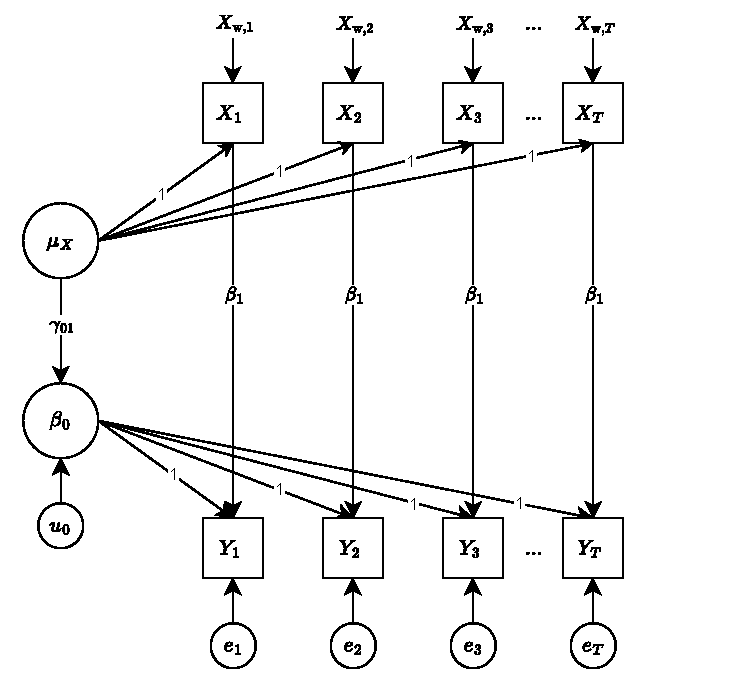
\includegraphics[height=6.5cm]{Figures/pathdiagrams-cropped-contxy.drawio.pdf}
            \caption{Continuous X and Y}\label{fig:path-contxy}
        \end{subfigure}
    \end{minipage}
    \hfill
    \begin{minipage}[t]{.49\linewidth}
        \centering
        \begin{subfigure}[b]{\linewidth}
            \centering
            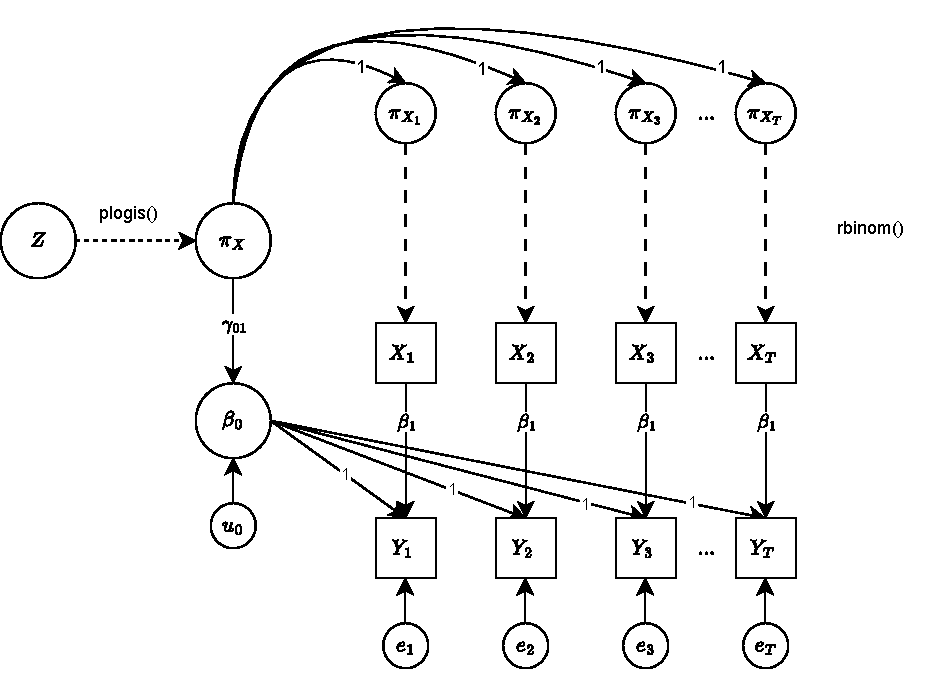
\includegraphics[height=6.5cm]{Figures/pathdiagrams-cropped-binxconty.drawio.pdf}
            \caption{Binary X and Continuous Y}\label{fig:path-binxconty}
        \end{subfigure}
    \end{minipage}

    % \vskip 1em

    % Bottom row
    \begin{minipage}[t]{.49\linewidth}
        \centering
        \begin{subfigure}[b]{\linewidth}
            \centering
            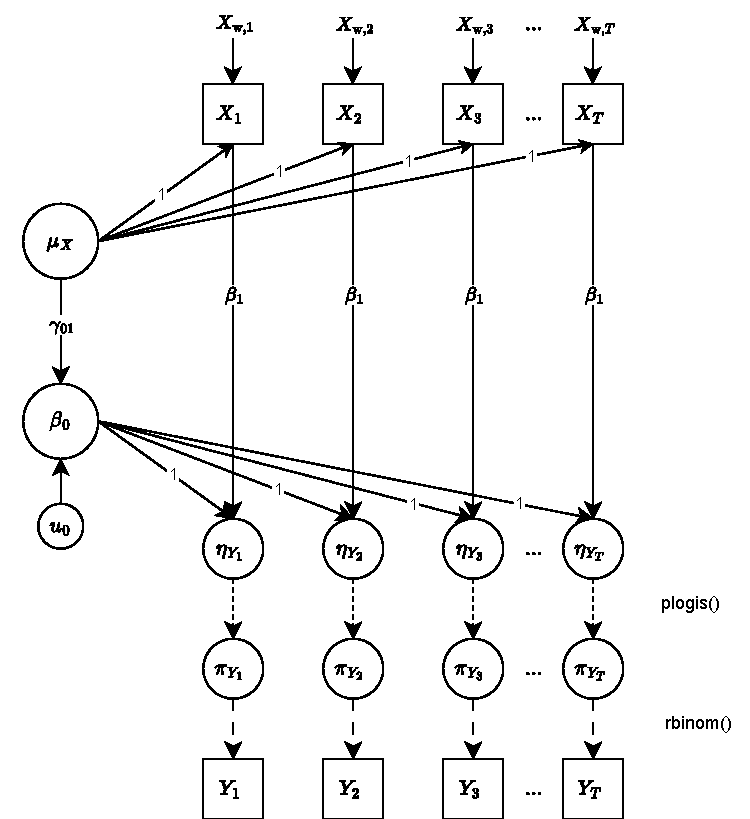
\includegraphics[height=7.5cm]{Figures/pathdiagrams-cropped-contxbiny.drawio.pdf}
            \caption{Continuous X and Binary Y}\label{fig:path-contxbiny}
        \end{subfigure}
    \end{minipage}
    \hfill
    \begin{minipage}[t]{.49\linewidth}
        \centering
        \begin{subfigure}[b]{\linewidth}
            \centering
            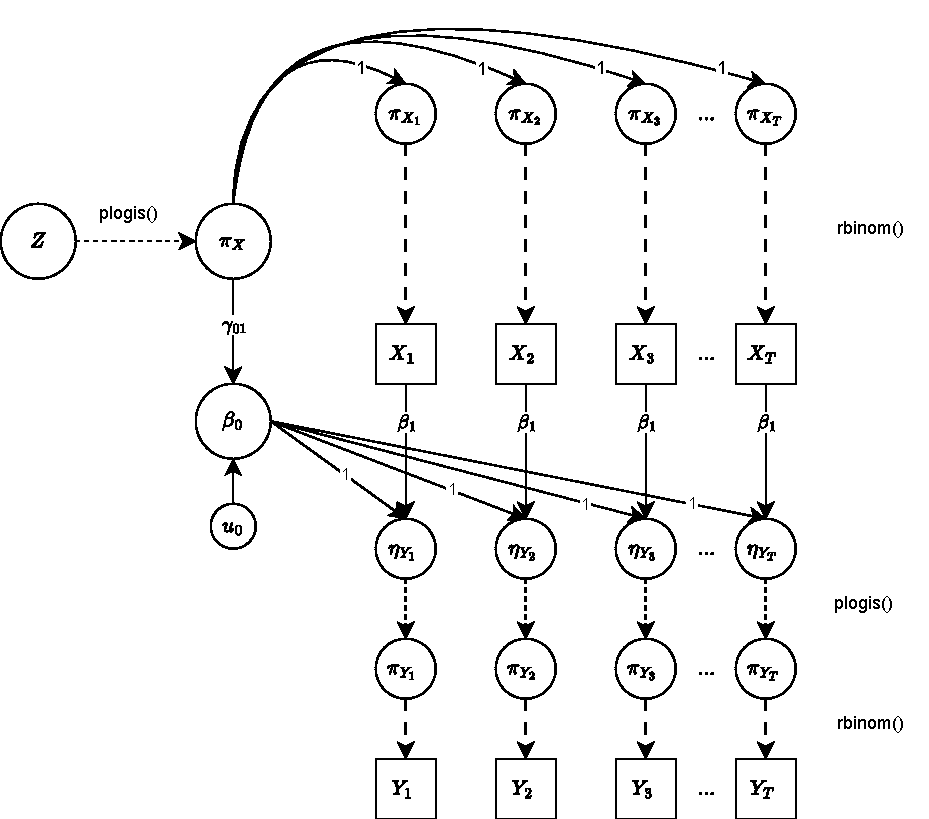
\includegraphics[height=7.5cm]{Figures/pathdiagrams-cropped-binxy.drawio.pdf}
            \caption{Binary X and Y}\label{fig:path-binxy}
        \end{subfigure}
    \end{minipage}
    \vspace{-0.5cm}
    \label{fig:path}
    \begin{flushleft}
    \begin{figurenote}
    Path diagrams of the four data-generating models, varying by predictor type $X$ (columns) and outcome type $Y$ (rows), each either continuous or binary. In all models, the outcome is regressed on the predictor, and the person-level predictor mean $\mu_X$ predicts the outcome intercept $\beta_0$, yielding a within-person slope $\beta_1$ and a contextual effect $\gamma_{01}$. Circles represent latent variables, squares observed variables. Solid arrows denote linear relations; dotted arrows indicate logit transformations (\texttt{plogis} in \texttt{R}); dashed arrows indicate Bernoulli sampling with probability $\pi$ (\texttt{rbinom} in \texttt{R}).
    
    % Path diagrams of four data generating models that vary in predictor type $X$ (column wise) and outcome type $Y$ (row wise), both of which are either continuous or binary. Models are based regressing the outcome variable on the predictor, while using the latent mean per person on the predictor $\mu_X$ to predict the intercept $\beta_{0}$ of the outcome. This results in the within-person slope $\beta_1$ and the contextual effect $\gamma_{01}$. Circles denote latent variables, squares denote observed variables, and arrows represent relationships. Solid arrows indicate linear associations, dotted arrows represent logit transformations (\texttt{plogis} in \texttt{R}), and dashed arrows indicate Bernoulli sampling with probability $\pi$ (\texttt{rbinom} in \texttt{R}).
    % Circles represent latent variables, squares represent observed variables, and arrows indicate relationships. Solid arrows denote linear associations, with a coefficient of 1 indicating a one-to-one relationship. Dotted arrows represent logit transformations (\texttt{plogis} in \texttt{R}), and dashed arrows represent Bernoulli sampling based on the probability $\pi$ (\texttt{rbinom} in \texttt{R}).
    \end{figurenote}
    \end{flushleft}
\end{center}

% \begin{center}
%     \captionof{figure}{Path diagrams of Generative Models with Within-Person ($\beta_1$) and Contextual Effect ($\gamma_{01}$)}
%     % Top row
%     \begin{minipage}[t]{.49\linewidth}
%         \centering
%         \begin{subfigure}[b]{\linewidth}
%             \centering
%             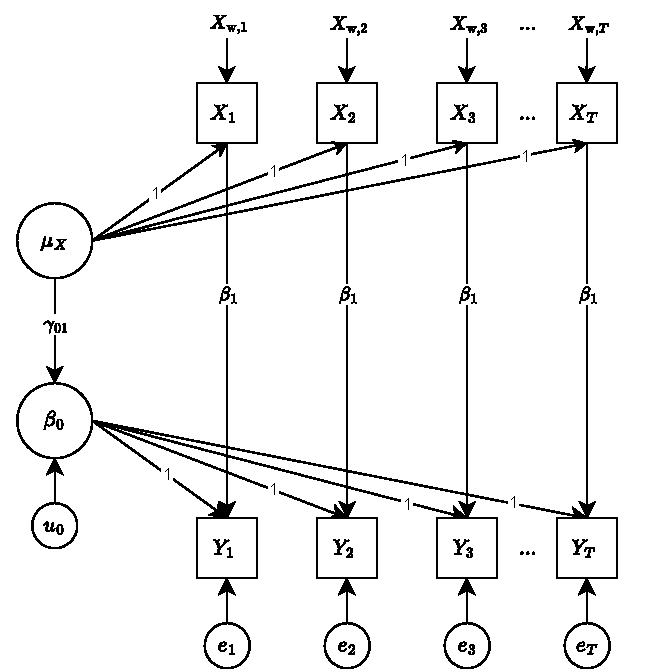
\includegraphics[width=\linewidth, height=8cm, keepaspectratio]{Figures/pathdiagrams-contxy.drawio.pdf}
%             \caption{Continuous X and Y}\label{fig:path-contxy}
%         \end{subfigure}
%     \end{minipage}
%     \hfill
%     \begin{minipage}[t]{.49\linewidth}
%         \centering
%         \begin{subfigure}[b]{\linewidth}
%             \centering
%             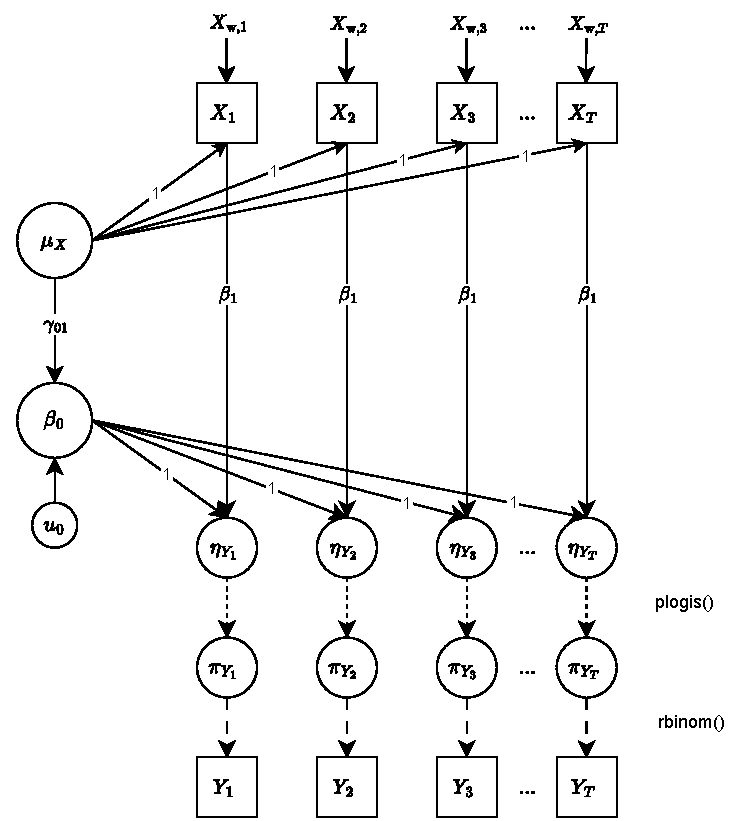
\includegraphics[width=\linewidth, height=8cm, keepaspectratio]{Figures/pathdiagrams-contxbiny.drawio.pdf}
%             \caption{Continuous X and Binary Y}\label{fig:path-contxbiny}
%         \end{subfigure}
%     \end{minipage}

%     % \vskip 1em

%     % Bottom row
%     \begin{minipage}[t]{.49\linewidth}
%         \centering
%         \begin{subfigure}[b]{\linewidth}
%             \centering
%             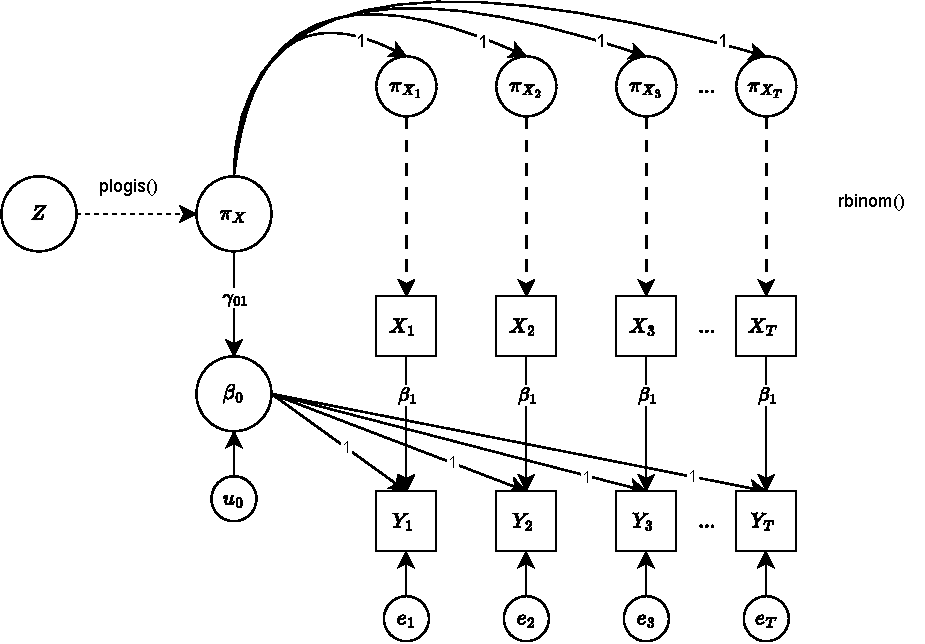
\includegraphics[width=\linewidth, height=8cm, keepaspectratio]{Figures/pathdiagrams-binxconty.drawio.pdf}
%             \caption{Binary X and Continuous Y}\label{fig:path-binxconty}
%         \end{subfigure}
%     \end{minipage}
%     \hfill
%     \begin{minipage}[t]{.49\linewidth}
%         \centering
%         \begin{subfigure}[b]{\linewidth}
%             \centering
%             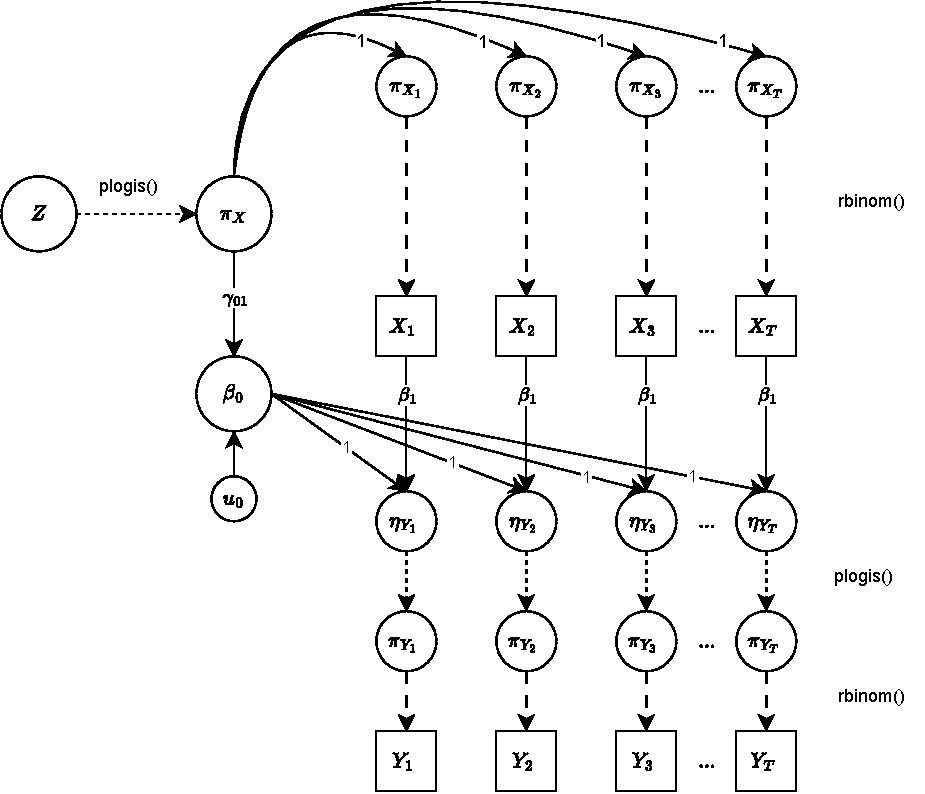
\includegraphics[width=\linewidth, height=8cm, keepaspectratio]{Figures/pathdiagrams-binxy.drawio.pdf}
%             \caption{Binary X and Y}\label{fig:path-binxy}
%         \end{subfigure}
%     \end{minipage}
%     \vspace{-1cm}
%     \label{fig:path}
%     \begin{flushleft}
%     \begin{figurenote}
%     Circles represent latent variables, squares represent observed variables, and arrows indicate relationships. Solid arrows denote linear associations, with a coefficient of 1 indicating a one-to-one relationship. Dotted arrows represent logit transformations (\texttt{plogis} in \texttt{R}), and dashed arrows represent Bernoulli sampling based on the probability $\pi$ (\texttt{rbinom} in \texttt{R}).
%     \end{figurenote}
%     \end{flushleft}
% \end{center}

% \begin{center}
% \captionof{figure}{Path diagrams of Generative Models with Within-Person ($\beta_\text{w}$) and Contextual Effect ($\gamma_{01}$)}

% \begin{minipage}[t]{.49\linewidth}
%     \centering
%     \begin{subfigure}[b]{\linewidth}
%         \centering
%         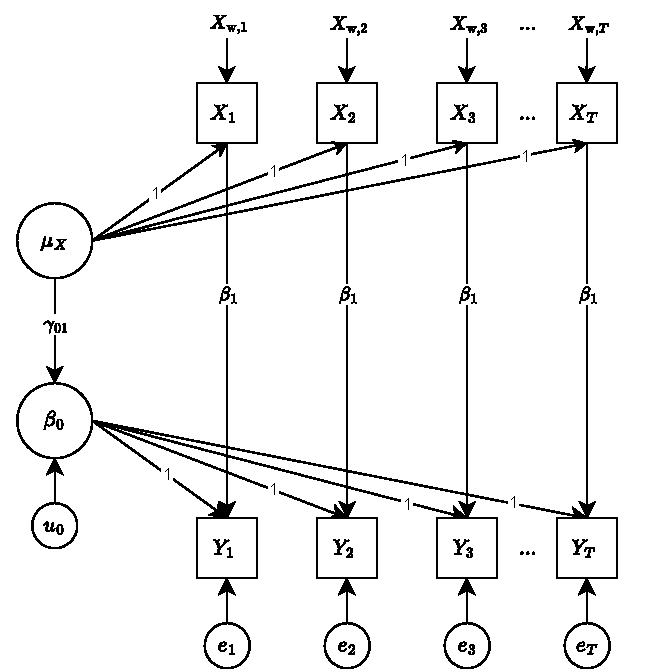
\includegraphics[width=\linewidth, height=8cm, keepaspectratio]{Figures/pathdiagrams-contxy.drawio.pdf}
%         \caption{Continuous X and Y}\label{fig:path-contxy}
%     \end{subfigure}
%     \vspace{1em}
%     \begin{subfigure}[b]{\linewidth}
%         \centering
%         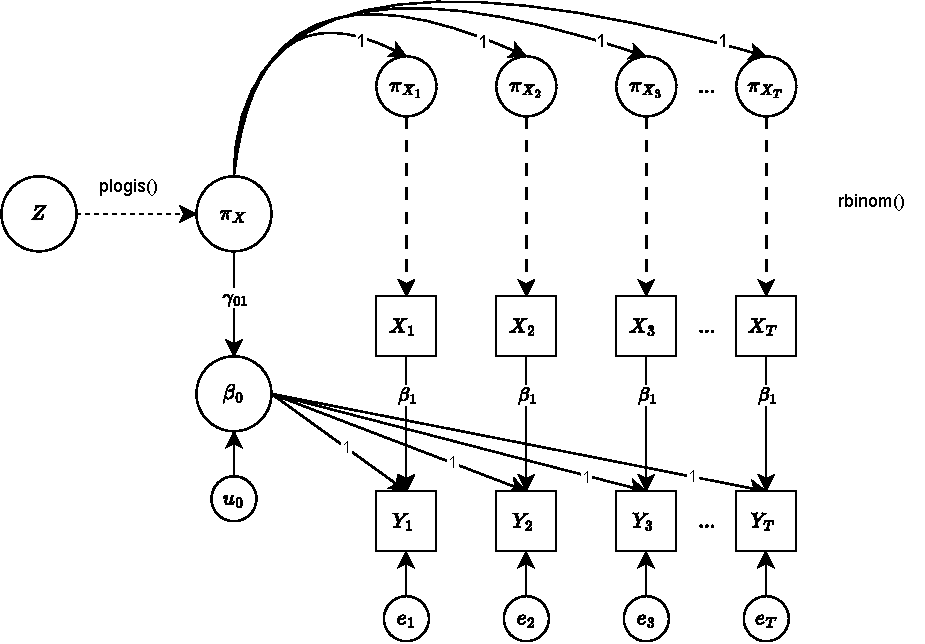
\includegraphics[width=\linewidth, height=8cm, keepaspectratio]{Figures/pathdiagrams-binxconty.drawio.pdf}
%         \caption{Binary X and Continuous Y}\label{fig:path-binxconty}
%     \end{subfigure}
% \end{minipage}
% \hfill
% \begin{minipage}[t]{.49\linewidth}
%     \centering
%     \begin{subfigure}[b]{\linewidth}
%         \centering
%         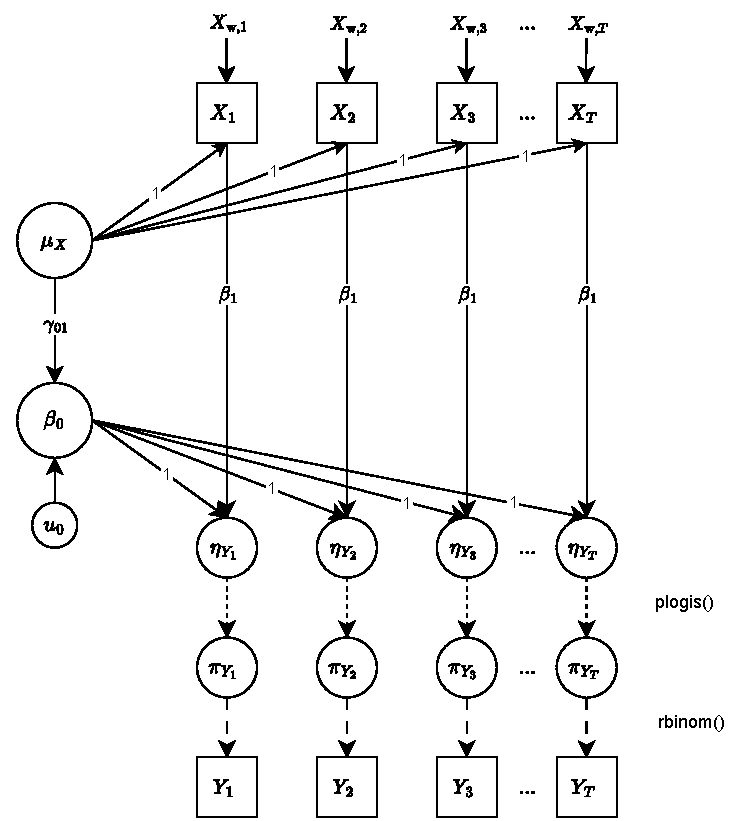
\includegraphics[width=\linewidth, height=8cm, keepaspectratio]{Figures/pathdiagrams-contxbiny.drawio.pdf}
%         \caption{Continuous X and Binary Y}\label{fig:path-contxbiny}
%     \end{subfigure}
%     \vspace{1em}
%     \begin{subfigure}[b]{\linewidth}
%         \centering
%         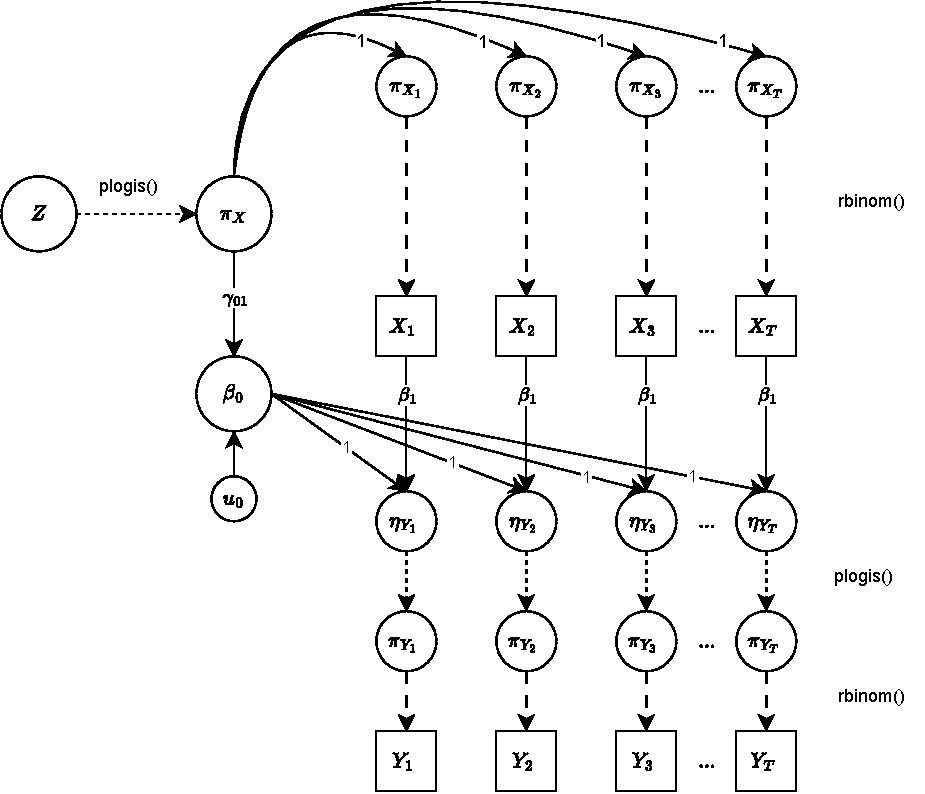
\includegraphics[width=\linewidth, height=8cm, keepaspectratio]{Figures/pathdiagrams-binxy.drawio.pdf}
%         \caption{Binary X and Y}\label{fig:path-binxy}
%     \end{subfigure}
% \end{minipage}

% \vspace{-0.5cm}
% \label{fig:path}

% \begin{flushleft}
% \begin{figurenote}
% Circles represent latent variables, squares represent observed variables, and arrows indicate relationships. Solid arrows denote linear associations, with a coefficient of 1 indicating a one-to-one relationship. Dotted arrows represent logit transformations (\texttt{plogis} in \texttt{R}), and dashed arrows represent Bernoulli sampling based on the probability $\pi$ (\texttt{rbinom} in \texttt{R}).
% \end{figurenote}
% \end{flushleft}
% \end{center}


To illustrate these DGMs, we use a running example grounded in prior empirical work on the effect of mindfulness (\(X_{it}\)) on anger (\(Y_{it}\)), where $X$ and $Y$ vary over individuals $i$ and time points $t$. Numerous studies have shown that, across individuals, those with higher overall mindfulness report lower overall levels of anger \parencite[]{brown_benefits_2003, borders_could_2010, kashdan_what_2016, baer_relationships_2011, eisenlohr-moul_both_2016}. Mindfulness also shows substantial within-person variability over time \parencite[]{brown_benefits_2003, kiken_state_2015}, and evidence suggests that on days when individuals report higher-than-usual mindfulness, they also report lower levels of state anger \parencite[]{eisenlohr-moul_both_2016}. Hence, both within- and between-person associations are negative, though effect sizes depend on the specific operationalization \parencite{eisenlohr-moul_both_2016}. Moreover, between-person associations tend to be larger, implying that a one-unit difference in average mindfulness between individuals is associated with a greater difference in anger-related outcomes than a one-unit increase in moment-to-moment fluctuations.


\subsection{DGM 1: Continuous Predictor and Outcome}

To illustrate the DGM for a continuous predictor and outcome, we consider the case of how mindfulness relates to daily experiences of anger (see Figure~\ref{fig:path-contxy}). Each individual possesses a stable level of trait mindfulness, denoted as a person-specific latent mean \( \mu_{X,i} \). This latent trait is assumed to vary across individuals according to a normal distribution $\mu_{X,i} \sim \mathcal{N}(0, \sigma^2_{X,\text{b}})$, where \( \sigma^2_{X,\text{b}} \) reflects the between-person variance in mindfulness. The observed $X$ for individual \( i \) at occasion \( t \), denoted \( X_{it} \), is a combination of an individual's stable trait level and a momentary deviation, and can thus be expressed as:
\begin{align}
    \label{eqn:relationwithinmundlak}
    X_{it} &= \mu_{X,i} + X_{\text{w},it}.
\end{align}
Here, \( X_{\text{w},it} \) represents the within-person score in mindfulness, capturing occasion-specific fluctuations around the person’s trait level. In Figure~\ref{fig:path-contxy}, the within-person score is obtained as $X_{\text{w},it} = X_{it} - \mu_{X,i}$. $X_{\text{w},it}$ varies over time according to a normal distribution \( X_{\text{w},it} \sim \mathcal{N}(0, \sigma^2_{X,\text{w}}) \), where \( \sigma^2_{X,\text{w}} \) reflects within-person variance in mindfulness. Daily anger, denoted \( Y_{it} \), is given by
\begin{equation}
    \label{eqn:yit-generationmlm}
    Y_{it} = \beta_{0i} + \beta_{1} X_{it} + e_{it},
\end{equation}
where \( \beta_{0i} \) is an individual-specific intercept capturing average levels of anger, and \( e_{it} \sim \mathcal{N}(0, \sigma^2_{e}) \) is a person- and time-specific residual with variance $\sigma^2_e$. The individual-specific intercept \( \beta_{0i} \) is a function of a person’s average mindfulness ($\mu_{X,i}$) through
\begin{equation}
    \label{eqn:beta0-generationcontxy}
    \beta_{0i} = \gamma_{00} + \gamma_{01} \mu_{X,i} + u_{0i},
\end{equation}
where \( \gamma_{00} \) is the grand mean of anger (given that $\mathrm{E} \left[ \mu_{X,i} \right] = 0$), and \( \gamma_{01} \) is the contextual effect of trait mindfulness on anger. The person-specific residual \( u_{0i} \sim \mathcal{N}(0, \sigma^2_u) \) is normally distributed with variance \( \sigma^2_u \), and represents residual heterogeneity in average anger between individuals after accounting for average levels of mindfulness. By substituting Equation~\ref{eqn:beta0-generationcontxy} into Equation~\ref{eqn:yit-generationmlm}, we obtain the combined expression:
\begin{equation}
    \label{eqn:dgm1-fulldgm}
    Y_{it} = \gamma_{00} + \gamma_{01} \mu_{X,i} + u_{0i} + \beta_1 X_{it} + e_{it}.
\end{equation}
In this DGM, there are two ways in which mindfulness ($X$) influences anger ($Y$). To make this explicit, we substitute Equation~\ref{eqn:relationwithinmundlak} into Equation~\ref{eqn:dgm1-fulldgm}, yielding:
\begin{equation}
    Y_{it} = \gamma_{00} + (\gamma_{01} + \beta_1) \mu_{X,i} + u_{0i} + \beta_1 X_{\text{w},it} + e_{it}.
\end{equation}
First, occasion-specific changes in mindfulness ($X_{\text{w},it}$) affect anger ($Y_{it}$) through the coefficient $\beta_1$, which represents the within-person effect: how anger changes on a given occasion when an individual is more or less mindful than usual. Between-person differences in average mindfulness ($\mu_{X,i}$) also influence anger, both through the term $\beta_1$ and via the contextual effect $\gamma_{01}$. The between-person effect—the impact of a person's typical mindfulness level (\( \mu_{X,i} \)) on average anger level—is given by $\beta_\text{b} = \gamma_{01} + \beta_1$ \parencite{mundlak_pooling_1978}.\footnote{This equivalence does not hold in the presence of \textit{random slopes}; see \textcite{snijders_multilevel_2011}.} If there is no contextual effect ($\gamma_{01} = 0$), the within- and between-person effects are equal and captured by $\beta_1$. Conversely, the presence of a contextual effect ($\gamma_{01} \neq 0$) implies that the between-person effect differs from the within-person effect. A positive \( \gamma_{01} \) indicates that individuals who are more mindful on average experience more anger than would be expected based only on the within-person relationship. A negative \( \gamma_{01} \) implies that individuals who are more mindful on average experience less anger than would be expected based solely on the within-person relationship.

Empirical work has found that the between-person effect tends to be larger in magnitude than the within-person effect \parencite[$\beta_\text{b} > \beta_1$;][]{eisenlohr-moul_both_2016}. As both effects are negative, this implies the presence of a \textit{negative} contextual effect. To reflect this, we employ the following parameter values: $
\gamma_{00} = 4.5,\quad \gamma_{01} = -0.5,\quad \beta_1 = -0.4$, which implies $\beta_\text{b} = -0.5 - 0.4 = -0.9$. As visualized in Figure~\ref{fig:withinbetween-contxy}, these parameters yield a stronger negative association at the between-person level than at the within-person level. We assume that the within-person effect is identical for both individuals and that these individuals vary only in their average levels of mindfulness and anger. Specifically, the individual depicted in orange has a distribution centered around a higher trait level of mindfulness ($\mu_{X,i} = 4$) than the individual depicted in red ($\mu_{X,i} = 2$). Due to the negative between-person effect of $X$ on $Y$, it follows that the individual in orange also has lower overall anger levels.

\newpage
\begin{center}
    \captionof{figure}{Illustration of Within- and Between-Person Effects in Generative Models with $\beta_1 = -0.4$}
    % Top row
    \begin{minipage}[t]{.45\linewidth}
        \centering
        \begin{subfigure}[b]{\linewidth}
            \centering
            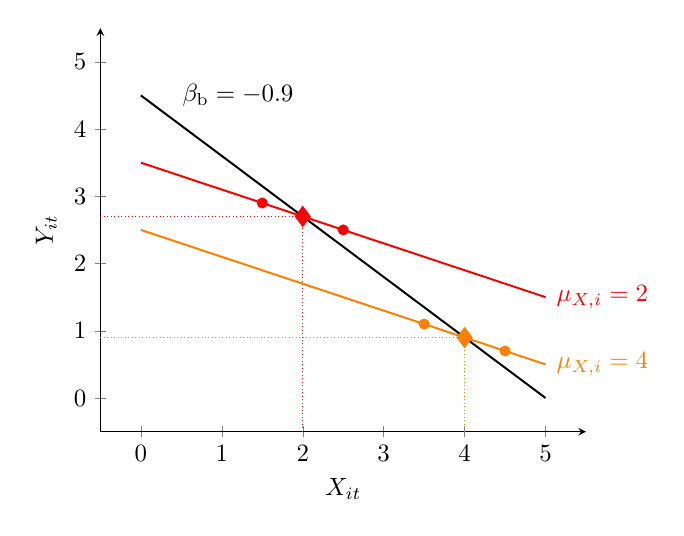
\begin{tikzpicture}[scale=0.9]
                \begin{axis}[
                    axis x line=left, 
                    axis y line=left, 
                    xlabel={$X_{it}$}, ylabel={$Y_{it}$},
                    xmin=0, xmax=5, ymin=0, ymax=5,
                    xtick={0,1,2,3,4,5},
                    ytick={0,1,2,3,4,5},
                    enlargelimits=true,
                    clip=false,
                    xshift=-15mm
                ]
            
                \pgfmathsetmacro{\gammaZero}{4.5}
                \pgfmathsetmacro{\gammaOne}{-0.5}
                \pgfmathsetmacro{\betaOne}{-0.4}
                \pgfmathsetmacro{\betaB}{-0.9}  % gamma01 + beta1
            
                % === Within-person: mu_X = 2 ===
                \addplot[domain=0:5, thick, red] {\gammaZero + \gammaOne*2 + \betaOne*x};
                \addplot[only marks, red] coordinates {
                    (1.5, {4.5 - 0.5*2 - 0.4*1.5})
                    % (2.0, {4.5 - 0.5*2 - 0.4*2.0})
                    (2.5, {4.5 - 0.5*2 - 0.4*2.5})
                };
                \addplot[only marks, mark=diamond*, mark size=4pt, red] coordinates {
                    (2.0, {4.5 - 0.5*2 - 0.4*2.0})
                };
                \addplot[densely dotted, thin, red] coordinates {
                    (2.0, -0.5)
                    (2.0, {4.5 - 0.5*2 - 0.4*2.0})
                };
                \addplot[densely dotted, thin, red] coordinates {
                    (-0.5, {4.5 - 0.5*2 - 0.4*2.0})
                    (2.0, {4.5 - 0.5*2 - 0.4*2.0})
                };
            
                % === Within-person: mu_X = 4 ===
                \addplot[domain=0:5, thick, orange] {\gammaZero + \gammaOne*4 + \betaOne*x};
                \addplot[only marks, orange] coordinates {
                    (3.5, {4.5 - 0.5*4 - 0.4*3.5})
                    % (4.0, {4.5 - 0.5*4 - 0.4*4.0})
                    (4.5, {4.5 - 0.5*4 - 0.4*4.5})
                };
                \addplot[only marks, mark=diamond*, mark size=4pt, orange] coordinates {
                    (4.0, {4.5 - 0.5*4 - 0.4*4.0})
                };
                \addplot[densely dotted, thin, orange] coordinates {
                    (4.0, -0.5)
                    (4.0, {4.5 - 0.5*4 - 0.4*4.0})
                };
                \addplot[densely dotted, thin, orange] coordinates {
                    (-0.5, {4.5 - 0.5*4 - 0.4*4})
                    (4.0, {4.5 - 0.5*4 - 0.4*4.0})
                };
            
                % === Between-person regression line ===
                \addplot[thick, black, domain=0:5] {\gammaZero + \betaB*x};
            
                % === Labels ===
                \node[red] at (axis cs:5.7,1.5) {$\mu_{X,i}=2$};
                \node[orange] at (axis cs:5.7,0.5) {$\mu_{X,i}=4$};
                \node[black] at (axis cs:1.2,4.5) {$\beta_\text{b} = -0.9$};
            
                \end{axis}
            \end{tikzpicture}
            \caption{Continuous X and Y}\label{fig:withinbetween-contxy}
        \end{subfigure}
    \end{minipage}
    \hfill
    \begin{minipage}[t]{.45\linewidth}
        \centering
        \begin{subfigure}[b]{\linewidth}
            \centering

            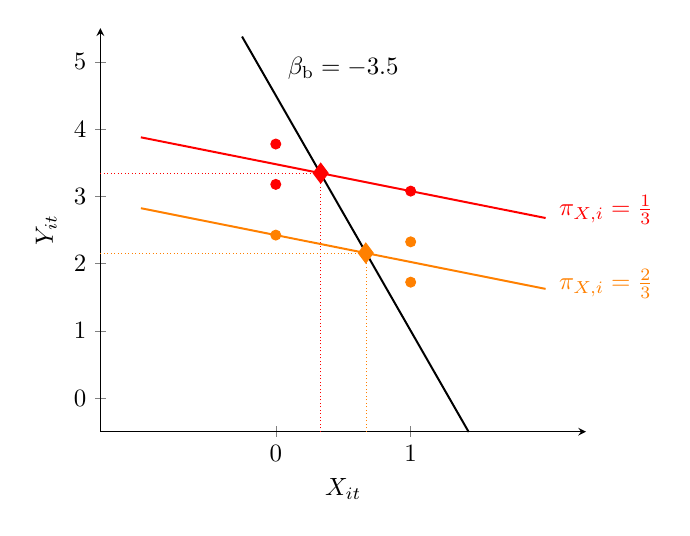
\begin{tikzpicture}[scale=0.9]
                \begin{axis}[
                    axis x line=left, 
                    axis y line=left, 
                    xlabel={$X_{it}$}, ylabel={$Y_{it}$},
                    xmin=-1, xmax=2, ymin=0, ymax=5,
                    xtick={0,1},
                    ytick={0,1,2,3,4,5},
                    enlargelimits=true,
                    clip=false,
                    xshift=-15mm,
                    samples=200,
                    domain=-1:2,
                ]
            
                \pgfmathsetmacro{\gammaZero}{4.5}
                \pgfmathsetmacro{\gammaOne}{-3.1}
                \pgfmathsetmacro{\betaOne}{-0.4}
                \pgfmathsetmacro{\betaB}{-3.5}
            
                % === Person with mu_X = 0.33 ===
                \pgfmathsetmacro{\muXone}{0.33}
                \pgfmathsetmacro{\intOne}{\gammaZero + \gammaOne*\muXone}
                \addplot[thick, red] coordinates {
                    (-1, {\intOne + \betaOne*-1})
                    (2, {\intOne + \betaOne*2})
                };
                \addplot[only marks, mark=diamond*, mark size=4pt, red] coordinates {
                (0.333, {\intOne + \betaOne*0.333})
                };
                \addplot[only marks, red] coordinates {
                    % (0, {\intOne + \betaOne*0})
                    (0, {\intOne + \betaOne*0.75})
                    (0, {\intOne + \betaOne*-0.75})
                    % (1, {\intOne + \betaOne*0.25})
                    (1, {\intOne + \betaOne*1})
                    % (1, {\intOne + \betaOne*1.75})
                };
                \addplot[densely dotted, thin, red] coordinates {
                    (\muXone, -0.5)
                    (\muXone, {\gammaZero + \betaB*\muXone})
                };
                \addplot[densely dotted, thin, red] coordinates {
                    (-1.3, {\gammaZero + \betaB*\muXone})
                    (\muXone, {\gammaZero + \betaB*\muXone})
                };
            
                % === Person with mu_X = 0.67 ===
                \pgfmathsetmacro{\muXtwo}{0.67}
                \pgfmathsetmacro{\intTwo}{\gammaZero + \gammaOne*\muXtwo}
                \addplot[thick, orange] coordinates {
                    (-1, {\intTwo + \betaOne*-1})
                    (2, {\intTwo + \betaOne*2})
                };
                \addplot[only marks, mark=diamond*, mark size=4pt, orange] coordinates {
                (0.667, {\intTwo + \betaOne*0.667})
                };
                \addplot[only marks, orange] coordinates {
                    (0, {\intTwo + \betaOne*0})
                    % (0, {\intTwo + \betaOne*0.75})
                    % (0, {\intTwo + \betaOne*-0.75})
                    (1, {\intTwo + \betaOne*0.25})
                    % (1, {\intTwo + \betaOne*1})
                    (1, {\intTwo + \betaOne*1.75})
                };
                \addplot[densely dotted, thin, orange] coordinates {
                    (\muXtwo, -0.5)
                    (\muXtwo, {\gammaZero + \betaB*\muXtwo})
                };
                \addplot[densely dotted, thin, orange] coordinates {
                    (-1.3, {\gammaZero + \betaB*\muXtwo})
                    (\muXtwo, {\gammaZero + \betaB*\muXtwo})
                };
            
                % === Between-person regression line ===
                \addplot[thick, black, domain=-0.25:1.43] {\gammaZero + \betaB*x};
            
                % === Labels ===
                \node[red] at (axis cs:2.45,2.8) {$\pi_{X,i}=\frac{1}{3}$};
                \node[orange] at (axis cs:2.45,1.7) {$\pi_{X,i}=\frac{2}{3}$};
                \node[black] at (axis cs:0.5,4.9) {$\beta_\text{b} = -3.5$};
            
                \end{axis}
            \end{tikzpicture}
            
            \caption{Binary X and Continuous Y}\label{fig:withinbetween-binxconty}
        \end{subfigure}
    \end{minipage}

    \vskip 1em

    % Bottom row
    \begin{minipage}[t]{.45\linewidth}
        \centering
        \begin{subfigure}[b]{\linewidth}
            \centering

            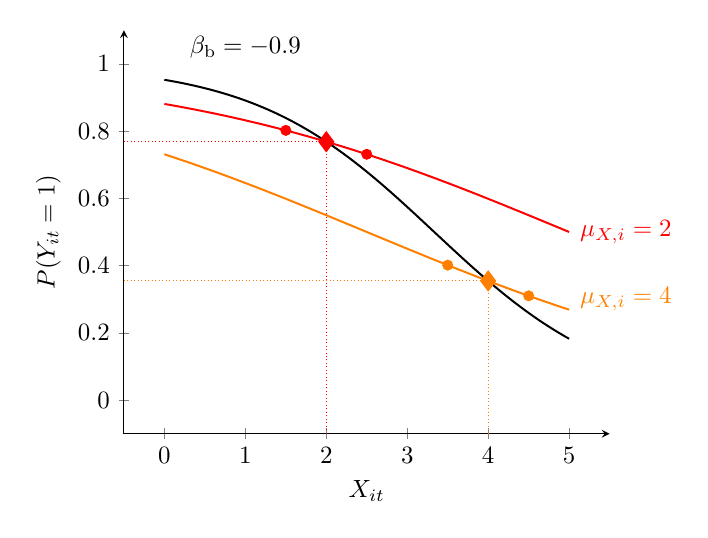
\begin{tikzpicture}[scale=0.9]
            \begin{axis}[
                axis x line=left, axis y line=left,
                xlabel={$X_{it}$}, ylabel={$P(Y_{it} = 1)$},
                xmin=0, xmax=5, ymin=0, ymax=1,
                % legend pos=south west,
                samples=200,
                domain=0:5,
                ytick={0,0.2,0.4,0.6,0.8,1},
                xtick={0,1,2,3,4,5},
                clip=false,
                enlargelimits=true
            ]
            
            % Parameters
            \pgfmathsetmacro{\gammaZero}{3}
            \pgfmathsetmacro{\gammaOne}{-0.5}
            \pgfmathsetmacro{\betaOne}{-0.4}
            \pgfmathsetmacro{\betaB}{-0.9}
            
            % Person 1: mu_X = 2
            \pgfmathsetmacro{\muXone}{2}
            \pgfmathsetmacro{\intOne}{\gammaZero + \gammaOne*\muXone}
            \addplot[red, thick] {1 / (1 + exp(-(\intOne + \betaOne*x)))};
            \addplot[only marks, mark=*, red] coordinates {
                (1.5, {1 / (1 + exp(-(\intOne + \betaOne*1.5)))})
                (2.5, {1 / (1 + exp(-(\intOne + \betaOne*2.5)))})
            };
            \addplot[only marks, mark=diamond*, mark size=4pt, red] coordinates {
                (2, {1 / (1 + exp(-(\intOne + \betaOne*2)))})
            };
            \addplot[densely dotted, thin, red] coordinates {
                (\muXone, -0.1)
                (\muXone, {1 / (1 + exp(-(\intOne + \betaOne*\muXone)))})
            };
            \addplot[densely dotted, thin, red] coordinates {
                (-0.5, {1 / (1 + exp(-(\intOne + \betaOne*\muXone)))})
                (\muXone, {1 / (1 + exp(-(\intOne + \betaOne*\muXone)))})
            };
            
            
            % Person 2: mu_X = 4
            \pgfmathsetmacro{\muXtwo}{4}
            \pgfmathsetmacro{\intTwo}{\gammaZero + \gammaOne*\muXtwo}
            \addplot[orange, thick] {1 / (1 + exp(-(\intTwo + \betaOne*x)))};
            \addplot[only marks, mark=*, orange] coordinates {
                (3.5, {1 / (1 + exp(-(\intTwo + \betaOne*3.5)))})
                (4.5, {1 / (1 + exp(-(\intTwo + \betaOne*4.5)))})
            };
            \addplot[only marks, mark=diamond*, mark size=4pt, orange] coordinates {
                (4, {1 / (1 + exp(-(\intTwo + \betaOne*4)))})
            };
            \addplot[densely dotted, thin, orange] coordinates {
            (\muXtwo, -0.1)
            (\muXtwo, {1 / (1 + exp(-(\intTwo + \betaOne*\muXtwo)))})
            };
            \addplot[densely dotted, thin, orange] coordinates {
            (-0.5, {1 / (1 + exp(-(\intTwo + \betaOne*\muXtwo)))})
            (\muXtwo, {1 / (1 + exp(-(\intTwo + \betaOne*\muXtwo)))})
            };
            
            % Between-person curve
            \addplot[black, thick] {1 / (1 + exp(-(\gammaZero + \betaB*x)))};
        
            % === Labels ===
            \node[red] at (axis cs:5.7,0.5) {$\mu_{X,i}=2$};
            \node[orange] at (axis cs:5.7,0.3) {$\mu_{X,i}=4$};
            \node[black] at (axis cs:1,1.05) {$\beta_\text{b} = -0.9$};
            
            
            \end{axis}
            \end{tikzpicture}
        
            \caption{Continuous X and Binary Y}\label{fig:withinbetween-contxbiny}
        \end{subfigure}
    \end{minipage}
    \hfill
    \begin{minipage}[t]{.45\linewidth}
        \centering
        \begin{subfigure}[b]{\linewidth}
            \centering
            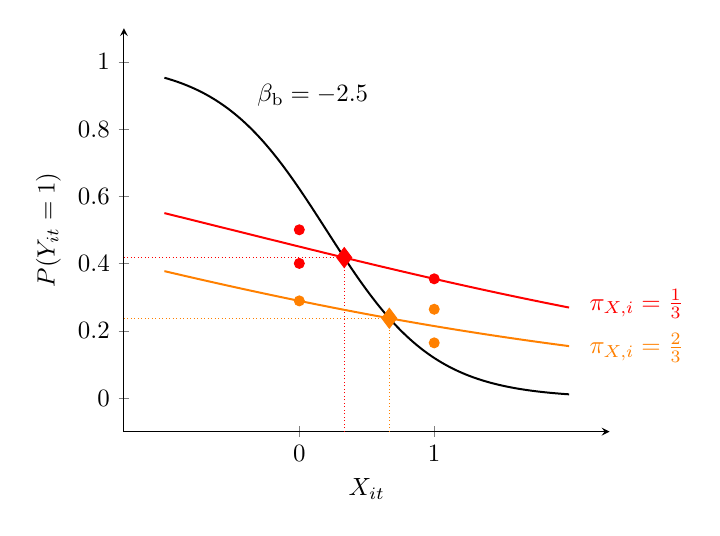
\begin{tikzpicture}[scale=0.9]
            \begin{axis}[
                axis x line=left, axis y line=left,
                xlabel={$X_{it}$}, ylabel={$P(Y_{it} = 1)$},
                xmin=-1, xmax=2, ymin=0, ymax=1,
                % legend pos=south west,
                samples=200,
                domain=-1:2,
                ytick={0,0.2,0.4,0.6,0.8,1},
                xtick={0,1},
                clip=false,
                enlargelimits=true
            ]
            
            % Parameters
            \pgfmathsetmacro{\gammaZero}{0.5}
            \pgfmathsetmacro{\gammaOne}{-2.1}
            \pgfmathsetmacro{\betaOne}{-0.4}
            \pgfmathsetmacro{\betaB}{-2.5}
            
            % Person 1: mu_X = 0.333
            \pgfmathsetmacro{\muXone}{0.333}
            \pgfmathsetmacro{\intOne}{\gammaZero + \gammaOne*\muXone}
            \addplot[red, thick] {1 / (1 + exp(-(\intOne + \betaOne*x)))};
            \addplot[only marks, mark=diamond*, mark size=4pt, red] coordinates {
                (0.333, {1 / (1 + exp(-(\intOne + \betaOne*0.333)))})
            };
            \addplot[only marks, mark=*, red] coordinates {
                % (0, {1 / (1 + exp(-(\intOne + \betaOne*0)))})
                (0, {1 / (1 + exp(-(\intOne + \betaOne*0))) + 0.05})
                (0, {1 / (1 + exp(-(\intOne + \betaOne*0))) - 0.05})
                (1, {1 / (1 + exp(-(\intOne + \betaOne*1)))})
                % (1, {1 / (1 + exp(-(\intOne + \betaOne*1))) + 0.05})
                % (1, {1 / (1 + exp(-(\intOne + \betaOne*1))) - 0.05})
            };
            \addplot[densely dotted, thin, red] coordinates {
                (\muXone, -0.1)
                (\muXone, {1 / (1 + exp(-(\intOne + \betaOne*\muXone)))})
            };
            \addplot[densely dotted, thin, red] coordinates {
                (-1.3, {1 / (1 + exp(-(\intOne + \betaOne*\muXone)))})
                (\muXone, {1 / (1 + exp(-(\intOne + \betaOne*\muXone)))})
            };
            
            % Person 2: mu_X = 0.667
            \pgfmathsetmacro{\muXtwo}{0.667}
            \pgfmathsetmacro{\intTwo}{\gammaZero + \gammaOne*\muXtwo}
            \addplot[orange, thick] {1 / (1 + exp(-(\intTwo + \betaOne*x)))};
            \addplot[only marks, mark=diamond*, mark size=4pt, orange] coordinates {
                (0.667, {1 / (1 + exp(-(\intTwo + \betaOne*0.667)))})
            };
            \addplot[only marks, mark=*, orange] coordinates {
                (0, {1 / (1 + exp(-(\intTwo + \betaOne*0)))})
                % (0, {1 / (1 + exp(-(\intTwo + \betaOne*0))) + 0.05})
                % (0, {1 / (1 + exp(-(\intTwo + \betaOne*0))) - 0.05})
                % (1, {1 / (1 + exp(-(\intTwo + \betaOne*1)))})
                (1, {1 / (1 + exp(-(\intTwo + \betaOne*1))) + 0.05})
                (1, {1 / (1 + exp(-(\intTwo + \betaOne*1))) - 0.05})
            };
            
            \addplot[densely dotted, thin, orange] coordinates {
            (\muXtwo, -0.1)
            (\muXtwo, {1 / (1 + exp(-(\intTwo + \betaOne*\muXtwo)))})
            };
            \addplot[densely dotted, thin, orange] coordinates {
            (-1.3, {1 / (1 + exp(-(\intTwo + \betaOne*\muXtwo)))})
            (\muXtwo, {1 / (1 + exp(-(\intTwo + \betaOne*\muXtwo)))})
            };
            
            % Between-person curve
            \addplot[black, thick] {1 / (1 + exp(-(\gammaZero + \betaB*x)))};
        
            % === Labels ===
            \node[red] at (axis cs:2.5,0.28){$\pi_{X,i}=\frac{1}{3}$};
            \node[orange] at (axis cs:2.5,0.15) {$\pi_{X,i}=\frac{2}{3}$};
            \node[black] at (axis cs:0.1,0.9) {$\beta_\text{b} = -2.5$};
            
            \end{axis}
        \end{tikzpicture}
        \caption{Binary X and Y}\label{fig:withinbetween-binxy}
        \end{subfigure}
    \end{minipage}
    
    \label{fig:path2}

    \vspace{-1cm}
    \begin{flushleft}
    \begin{figurenote}
    Within-person effects ($\beta_1$) and between-person effects ($\beta_b$) are shown for data-generating mechanisms varying by predictor type $X$ (columns) and outcome type $Y$ (rows), each either continuous or binary. For continuous outcomes, relationships are linear; for binary outcomes, the Y-axis reflects the probability of $Y = 1$, and relationships follow a logistic curve. The solid black line denotes the between-person effect; colored lines represent within-person effects for two individuals. Circles are hypothetical observations; diamonds mark where each within-person slope intersects the between-person slope. Thin dotted lines indicate each person's mean on $X$ and $Y$.
    
    % The within-person effects $\beta_1$ and between-person effects $\beta_\text{b}$ illustrated for data-generating mechanisms that vary by predictor type $X$ (columns) and outcome type $Y$ (rows), each either continuous or binary. For continuous outcomes, the relationship between $X$ and $Y$ are linear, whereas for binary outcomes the Y-axis represents a probability of scoring 1, where the effects have a logistic curves.
    % The solid black line represents the \textit{between-person} effect, while the colored solid lines indicate \textit{within-person} effects for two individuals. Circles represent hypothetical observations. Diamonds mark the point where each individual's within-person slope intersects with the between-person slope, and the thin colored dotted lines indicate that individual’s average on on $X$ and on $Y$.
    \end{figurenote}
    \end{flushleft}
\end{center}

% \begin{center}
%     \captionof{figure}{Within- and Between-Person Effects in Data Generating Models with $\beta_\text{w} = -0.4$}
%     % Top row
%     \begin{minipage}[t]{.45\linewidth}
%         \centering
%         \begin{subfigure}[b]{\linewidth}
%             \centering
%             \begin{tikzpicture}
%                 \begin{axis}[
%                     axis x line=left, 
%                     axis y line=left, 
%                     xlabel={$X_{it}$}, ylabel={$Y_{it}$},
%                     xmin=0, xmax=5, ymin=0, ymax=5,
%                     xtick={0,1,2,3,4,5},
%                     ytick={0,1,2,3,4,5},
%                     enlargelimits=true,
%                     clip=false,
%                     xshift=-15mm
%                 ]
            
%                 \pgfmathsetmacro{\gammaZero}{4.5}
%                 \pgfmathsetmacro{\gammaOne}{-0.5}
%                 \pgfmathsetmacro{\betaOne}{-0.4}
%                 \pgfmathsetmacro{\betaB}{-0.9}  % gamma01 + beta1
            
%                 % === Within-person: mu_X = 2 ===
%                 \addplot[domain=0:5, thick, red] {\gammaZero + \gammaOne*2 + \betaOne*x};
%                 \addplot[only marks, red] coordinates {
%                     (1.5, {4.5 - 0.5*2 - 0.4*1.5})
%                     % (2.0, {4.5 - 0.5*2 - 0.4*2.0})
%                     (2.5, {4.5 - 0.5*2 - 0.4*2.5})
%                 };
%                 \addplot[only marks, mark=diamond*, mark size=4pt, red] coordinates {
%                     (2.0, {4.5 - 0.5*2 - 0.4*2.0})
%                 };
%                 \addplot[densely dotted, thin, red] coordinates {
%                     (2.0, -0.5)
%                     (2.0, {4.5 - 0.5*2 - 0.4*2.0})
%                 };
%                 \addplot[densely dotted, thin, red] coordinates {
%                     (-0.5, {4.5 - 0.5*2 - 0.4*2.0})
%                     (2.0, {4.5 - 0.5*2 - 0.4*2.0})
%                 };
            
%                 % === Within-person: mu_X = 4 ===
%                 \addplot[domain=0:5, thick, orange] {\gammaZero + \gammaOne*4 + \betaOne*x};
%                 \addplot[only marks, orange] coordinates {
%                     (3.5, {4.5 - 0.5*4 - 0.4*3.5})
%                     % (4.0, {4.5 - 0.5*4 - 0.4*4.0})
%                     (4.5, {4.5 - 0.5*4 - 0.4*4.5})
%                 };
%                 \addplot[only marks, mark=diamond*, mark size=4pt, orange] coordinates {
%                     (4.0, {4.5 - 0.5*4 - 0.4*4.0})
%                 };
%                 \addplot[densely dotted, thin, orange] coordinates {
%                     (4.0, -0.5)
%                     (4.0, {4.5 - 0.5*4 - 0.4*4.0})
%                 };
%                 \addplot[densely dotted, thin, orange] coordinates {
%                     (-0.5, {4.5 - 0.5*4 - 0.4*4})
%                     (4.0, {4.5 - 0.5*4 - 0.4*4.0})
%                 };
            
%                 % === Between-person regression line ===
%                 \addplot[thick, black, domain=0:5] {\gammaZero + \betaB*x};
            
%                 % === Labels ===
%                 \node[red] at (axis cs:5.7,1.5) {$\mu_{X,i}=2$};
%                 \node[orange] at (axis cs:5.7,0.5) {$\mu_{X,i}=4$};
%                 \node[black] at (axis cs:1.2,4.5) {$\beta_\text{b} = -0.9$};
            
%                 \end{axis}
%             \end{tikzpicture}
%             \caption{Continuous X and Y}\label{fig:withinbetween-contxy}
%         \end{subfigure}
%     \end{minipage}
%     \hfill
%     \begin{minipage}[t]{.45\linewidth}
%         \centering
%         \begin{subfigure}[b]{\linewidth}
%             \centering
%             \begin{tikzpicture}
%             \begin{axis}[
%                 axis x line=left, axis y line=left,
%                 xlabel={$X_{it}$}, ylabel={$P(Y_{it} = 1)$},
%                 xmin=0, xmax=5, ymin=0, ymax=1,
%                 % legend pos=south west,
%                 samples=200,
%                 domain=0:5,
%                 ytick={0,0.2,0.4,0.6,0.8,1},
%                 xtick={0,1,2,3,4,5},
%                 clip=false,
%                 enlargelimits=true
%             ]
            
%             % Parameters
%             \pgfmathsetmacro{\gammaZero}{3}
%             \pgfmathsetmacro{\gammaOne}{-0.5}
%             \pgfmathsetmacro{\betaOne}{-0.4}
%             \pgfmathsetmacro{\betaB}{-0.9}
            
%             % Person 1: mu_X = 2
%             \pgfmathsetmacro{\muXone}{2}
%             \pgfmathsetmacro{\intOne}{\gammaZero + \gammaOne*\muXone}
%             \addplot[red, thick] {1 / (1 + exp(-(\intOne + \betaOne*x)))};
%             \addplot[only marks, mark=*, red] coordinates {
%                 (1.5, {1 / (1 + exp(-(\intOne + \betaOne*1.5)))})
%                 (2.5, {1 / (1 + exp(-(\intOne + \betaOne*2.5)))})
%             };
%             \addplot[only marks, mark=diamond*, mark size=4pt, red] coordinates {
%                 (2, {1 / (1 + exp(-(\intOne + \betaOne*2)))})
%             };
%             \addplot[densely dotted, thin, red] coordinates {
%                 (\muXone, -0.1)
%                 (\muXone, {1 / (1 + exp(-(\intOne + \betaOne*\muXone)))})
%             };
%             \addplot[densely dotted, thin, red] coordinates {
%                 (-0.5, {1 / (1 + exp(-(\intOne + \betaOne*\muXone)))})
%                 (\muXone, {1 / (1 + exp(-(\intOne + \betaOne*\muXone)))})
%             };
            
            
%             % Person 2: mu_X = 4
%             \pgfmathsetmacro{\muXtwo}{4}
%             \pgfmathsetmacro{\intTwo}{\gammaZero + \gammaOne*\muXtwo}
%             \addplot[orange, thick] {1 / (1 + exp(-(\intTwo + \betaOne*x)))};
%             \addplot[only marks, mark=*, orange] coordinates {
%                 (3.5, {1 / (1 + exp(-(\intTwo + \betaOne*3.5)))})
%                 (4.5, {1 / (1 + exp(-(\intTwo + \betaOne*4.5)))})
%             };
%             \addplot[only marks, mark=diamond*, mark size=4pt, orange] coordinates {
%                 (4, {1 / (1 + exp(-(\intTwo + \betaOne*4)))})
%             };
%             \addplot[densely dotted, thin, orange] coordinates {
%             (\muXtwo, -0.1)
%             (\muXtwo, {1 / (1 + exp(-(\intTwo + \betaOne*\muXtwo)))})
%             };
%             \addplot[densely dotted, thin, orange] coordinates {
%             (-0.5, {1 / (1 + exp(-(\intTwo + \betaOne*\muXtwo)))})
%             (\muXtwo, {1 / (1 + exp(-(\intTwo + \betaOne*\muXtwo)))})
%             };
            
%             % Between-person curve
%             \addplot[black, thick] {1 / (1 + exp(-(\gammaZero + \betaB*x)))};
        
%             % === Labels ===
%             \node[red] at (axis cs:5.7,0.5) {$\mu_{X,i}=2$};
%             \node[orange] at (axis cs:5.7,0.3) {$\mu_{X,i}=4$};
%             \node[black] at (axis cs:1,1.05) {$\beta_\text{b} = -0.9$};
            
            
%             \end{axis}
%         \end{tikzpicture}
%             \caption{Continuous X and Binary Y}\label{fig:withinbetween-contxbiny}
%         \end{subfigure}
%     \end{minipage}

%     \vskip 1em

%     % Bottom row
%     \begin{minipage}[t]{.45\linewidth}
%         \centering
%         \begin{subfigure}[b]{\linewidth}
%             \centering
%             \begin{tikzpicture}
%                 \begin{axis}[
%                     axis x line=left, 
%                     axis y line=left, 
%                     xlabel={$X_{it}$}, ylabel={$Y_{it}$},
%                     xmin=-1, xmax=2, ymin=0, ymax=5,
%                     xtick={0,1},
%                     ytick={0,1,2,3,4,5},
%                     enlargelimits=true,
%                     clip=false,
%                     xshift=-15mm,
%                     samples=200,
%                     domain=-1:2,
%                 ]
            
%                 \pgfmathsetmacro{\gammaZero}{4.5}
%                 \pgfmathsetmacro{\gammaOne}{-3.1}
%                 \pgfmathsetmacro{\betaOne}{-0.4}
%                 \pgfmathsetmacro{\betaB}{-3.5}
            
%                 % === Person with mu_X = 0.33 ===
%                 \pgfmathsetmacro{\muXone}{0.33}
%                 \pgfmathsetmacro{\intOne}{\gammaZero + \gammaOne*\muXone}
%                 \addplot[thick, red] coordinates {
%                     (-1, {\intOne + \betaOne*-1})
%                     (2, {\intOne + \betaOne*2})
%                 };
%                 \addplot[only marks, mark=diamond*, mark size=4pt, red] coordinates {
%                 (0.333, {\intOne + \betaOne*0.333})
%                 };
%                 \addplot[only marks, red] coordinates {
%                     % (0, {\intOne + \betaOne*0})
%                     (0, {\intOne + \betaOne*0.75})
%                     (0, {\intOne + \betaOne*-0.75})
%                     % (1, {\intOne + \betaOne*0.25})
%                     (1, {\intOne + \betaOne*1})
%                     % (1, {\intOne + \betaOne*1.75})
%                 };
%                 \addplot[densely dotted, thin, red] coordinates {
%                     (\muXone, -0.5)
%                     (\muXone, {\gammaZero + \betaB*\muXone})
%                 };
%                 \addplot[densely dotted, thin, red] coordinates {
%                     (-1.3, {\gammaZero + \betaB*\muXone})
%                     (\muXone, {\gammaZero + \betaB*\muXone})
%                 };
            
%                 % === Person with mu_X = 0.67 ===
%                 \pgfmathsetmacro{\muXtwo}{0.67}
%                 \pgfmathsetmacro{\intTwo}{\gammaZero + \gammaOne*\muXtwo}
%                 \addplot[thick, orange] coordinates {
%                     (-1, {\intTwo + \betaOne*-1})
%                     (2, {\intTwo + \betaOne*2})
%                 };
%                 \addplot[only marks, mark=diamond*, mark size=4pt, orange] coordinates {
%                 (0.667, {\intTwo + \betaOne*0.667})
%                 };
%                 \addplot[only marks, orange] coordinates {
%                     (0, {\intTwo + \betaOne*0})
%                     % (0, {\intTwo + \betaOne*0.75})
%                     % (0, {\intTwo + \betaOne*-0.75})
%                     (1, {\intTwo + \betaOne*0.25})
%                     % (1, {\intTwo + \betaOne*1})
%                     (1, {\intTwo + \betaOne*1.75})
%                 };
%                 \addplot[densely dotted, thin, orange] coordinates {
%                     (\muXtwo, -0.5)
%                     (\muXtwo, {\gammaZero + \betaB*\muXtwo})
%                 };
%                 \addplot[densely dotted, thin, orange] coordinates {
%                     (-1.3, {\gammaZero + \betaB*\muXtwo})
%                     (\muXtwo, {\gammaZero + \betaB*\muXtwo})
%                 };
            
%                 % === Between-person regression line ===
%                 \addplot[thick, black, domain=-0.25:1.43] {\gammaZero + \betaB*x};
            
%                 % === Labels ===
%                 \node[red] at (axis cs:2.45,2.8) {$\pi_{X,i}=\frac{1}{3}$};
%                 \node[orange] at (axis cs:2.45,1.7) {$\pi_{X,i}=\frac{2}{3}$};
%                 \node[black] at (axis cs:0.5,4.9) {$\beta_\text{b} = -3.5$};
            
%                 \end{axis}
%             \end{tikzpicture}
%             \caption{Binary X and Continuous Y}\label{fig:withinbetween-binxconty}
%         \end{subfigure}
%     \end{minipage}
%     \hfill
%     \begin{minipage}[t]{.45\linewidth}
%         \centering
%         \begin{subfigure}[b]{\linewidth}
%             \centering
%             \begin{tikzpicture}
%             \begin{axis}[
%                 axis x line=left, axis y line=left,
%                 xlabel={$X_{it}$}, ylabel={$P(Y_{it} = 1)$},
%                 xmin=-1, xmax=2, ymin=0, ymax=1,
%                 % legend pos=south west,
%                 samples=200,
%                 domain=-1:2,
%                 ytick={0,0.2,0.4,0.6,0.8,1},
%                 xtick={0,1},
%                 clip=false,
%                 enlargelimits=true
%             ]
            
%             % Parameters
%             \pgfmathsetmacro{\gammaZero}{0.5}
%             \pgfmathsetmacro{\gammaOne}{-2.1}
%             \pgfmathsetmacro{\betaOne}{-0.4}
%             \pgfmathsetmacro{\betaB}{-2.5}
            
%             % Person 1: mu_X = 0.333
%             \pgfmathsetmacro{\muXone}{0.333}
%             \pgfmathsetmacro{\intOne}{\gammaZero + \gammaOne*\muXone}
%             \addplot[red, thick] {1 / (1 + exp(-(\intOne + \betaOne*x)))};
%             \addplot[only marks, mark=diamond*, mark size=4pt, red] coordinates {
%                 (0.333, {1 / (1 + exp(-(\intOne + \betaOne*0.333)))})
%             };
%             \addplot[only marks, mark=*, red] coordinates {
%                 % (0, {1 / (1 + exp(-(\intOne + \betaOne*0)))})
%                 (0, {1 / (1 + exp(-(\intOne + \betaOne*0))) + 0.05})
%                 (0, {1 / (1 + exp(-(\intOne + \betaOne*0))) - 0.05})
%                 (1, {1 / (1 + exp(-(\intOne + \betaOne*1)))})
%                 % (1, {1 / (1 + exp(-(\intOne + \betaOne*1))) + 0.05})
%                 % (1, {1 / (1 + exp(-(\intOne + \betaOne*1))) - 0.05})
%             };
%             \addplot[densely dotted, thin, red] coordinates {
%                 (\muXone, -0.1)
%                 (\muXone, {1 / (1 + exp(-(\intOne + \betaOne*\muXone)))})
%             };
%             \addplot[densely dotted, thin, red] coordinates {
%                 (-1.3, {1 / (1 + exp(-(\intOne + \betaOne*\muXone)))})
%                 (\muXone, {1 / (1 + exp(-(\intOne + \betaOne*\muXone)))})
%             };
            
%             % Person 2: mu_X = 0.667
%             \pgfmathsetmacro{\muXtwo}{0.667}
%             \pgfmathsetmacro{\intTwo}{\gammaZero + \gammaOne*\muXtwo}
%             \addplot[orange, thick] {1 / (1 + exp(-(\intTwo + \betaOne*x)))};
%             \addplot[only marks, mark=diamond*, mark size=4pt, orange] coordinates {
%                 (0.667, {1 / (1 + exp(-(\intTwo + \betaOne*0.667)))})
%             };
%             \addplot[only marks, mark=*, orange] coordinates {
%                 (0, {1 / (1 + exp(-(\intTwo + \betaOne*0)))})
%                 % (0, {1 / (1 + exp(-(\intTwo + \betaOne*0))) + 0.05})
%                 % (0, {1 / (1 + exp(-(\intTwo + \betaOne*0))) - 0.05})
%                 % (1, {1 / (1 + exp(-(\intTwo + \betaOne*1)))})
%                 (1, {1 / (1 + exp(-(\intTwo + \betaOne*1))) + 0.05})
%                 (1, {1 / (1 + exp(-(\intTwo + \betaOne*1))) - 0.05})
%             };
            
%             \addplot[densely dotted, thin, orange] coordinates {
%             (\muXtwo, -0.1)
%             (\muXtwo, {1 / (1 + exp(-(\intTwo + \betaOne*\muXtwo)))})
%             };
%             \addplot[densely dotted, thin, orange] coordinates {
%             (-1.3, {1 / (1 + exp(-(\intTwo + \betaOne*\muXtwo)))})
%             (\muXtwo, {1 / (1 + exp(-(\intTwo + \betaOne*\muXtwo)))})
%             };
            
%             % Between-person curve
%             \addplot[black, thick] {1 / (1 + exp(-(\gammaZero + \betaB*x)))};
        
%             % === Labels ===
%             \node[red] at (axis cs:2.5,0.28){$\pi_{X,i}=\frac{1}{3}$};
%             \node[orange] at (axis cs:2.5,0.15) {$\pi_{X,i}=\frac{2}{3}$};
%             \node[black] at (axis cs:0.1,0.9) {$\beta_\text{b} = -2.5$};
            
%             \end{axis}
%         \end{tikzpicture}
%         \caption{Binary X and Y}\label{fig:withinbetween-binxy}
%         \end{subfigure}
%     \end{minipage}
    
%     \label{fig:path2}

%     % \vspace{-2cm}
%     \begin{flushleft}
%     \begin{figurenote}
%     The solid black line represents the \textit{between-person} effect, while the colored solid lines indicate \textit{within-person} effects for each individual. Circles represent hypothetical observations. Diamonds mark the point where each individual's within-person slope intersects with the between-person slope, and the thin colored dotted lines indicate that individual’s average on on $X$ and on $Y$.
%     \end{figurenote}
%     \end{flushleft}
% \end{center}


\subsection{DGM 2: Binary Predictor and Continuous Outcome}

To illustrate the DGM for a binary predictor and continuous outcome, we consider the case where daily engagement in a mindfulness practice (e.g., meditation), coded as 1 if practiced and 0 otherwise, influences experiences of anger (see Figure~\ref{fig:path-binxconty}). Each individual is characterized by a latent propensity to engage in mindfulness on a given day, denoted \( Z_i \), which varies across individuals according to a normal distribution \( Z_i \sim \mathcal{N}(0, \sigma^2_{Z}) \). This continuous latent trait is transformed via a logistic function to yield the individual-specific probability \( \pi_{X,i} \in (0,1) \)---taking on values strictly between 0 and 1---of engaging in mindfulness:
\begin{align}
    \label{eqn:dgm2-level2X}
    \pi_{X,i} &= \frac{e^{Z_i}}{1+ e^{Z_i}}.
\end{align}
The observed mindfulness practice score \( X_{it} \in \{0,1\} \) for individual \( i \) at occasion \( t \) is a \textit{binary} variable determined by the underlying probability \( \pi_{X,i} \) and a Bernoulli sampling process: \( X_{it} \sim \text{Bernoulli}(\pi_{X,i}) \). In this way, each person’s binary predictor values vary across time due to probabilistic sampling, and the extent of within-person variability is a function of their underlying propensity \( \pi_{X,i} \). Individuals with extreme trait probabilities (close to 0 or 1) will show little within-person variation, whereas those with moderate probabilities will exhibit more fluctuation.

Anger on day \( t \) for person \( i \), denoted \( Y_{it} \), is determined by the person’s observed mindfulness practice \( X_{it} \), a person-specific intercept \( \beta_{0i} \), and a residual \( e_{it} \) (see Equation~\ref{eqn:yit-generationmlm}). The random intercept \( \beta_{0i} \) is a function of \( \pi_{X,i} \) via
\begin{equation}
    \label{eqn:dgm2-betweenlevel}
    \beta_{0i} = \gamma_{00} + \gamma_{01} \pi_{X,i} + u_{0i},
\end{equation}
where $\gamma_{00}$ represents the extrapolated anger level for a hypothetical individual with an extreme aversion to mindfulness practice (with $\pi_{X,i} = 0$), \( \gamma_{01} \) is the contextual effect of average mindfulness engagement, and \( u_{0i} \sim \mathcal{N}(0, \sigma^2_u) \) captures person-level heterogeneity unexplained by \( \pi_{X,i} \). Substituting Equation~\ref{eqn:dgm2-betweenlevel} into Equation~\ref{eqn:yit-generationmlm} yields the composite model:
\begin{equation}
    Y_{it} = \gamma_{00} + \gamma_{01} \pi_{X,i} + u_{0i} + \beta_1 X_{it} + e_{it}.
\end{equation}
This DGM captures two distinct effects of mindfulness practice (\( X \)) on anger (\( Y \)). Within-person fluctuations in mindfulness engagement influence anger (\( Y_{it} \)) through \( \beta_1 \), reflecting how anger changes on days with versus without mindfulness practice. Between-person differences in the general tendency to practice mindfulness (\( \pi_{X,i} \)) influence anger both through \( \beta_1 \) and via the contextual effect \( \gamma_{01} \). Accordingly, the contextual effect \( \gamma_{01} \) captures whether individuals who typically engage more in mindfulness experience systematically different anger levels than expected based on their day-to-day engagement alone. 

Let us consider a plausible generative structure, where \( \gamma_{00} = 4.5, \quad \gamma_{01} = -3.1, \quad \beta_1 = -0.4 \), resulting in a between-person effect of \( \beta_\text{b} = -3.5 \). This pattern, visualized in Figure~\ref{fig:withinbetween-binxconty}, suggests that individuals who engage in mindfulness more frequently benefit from reduced anger than expected based on their day-to-day practice alone. The two individuals vary only in their propensity to engage in mindfulness and average anger. The person indicated in orange has a higher overall probability of practicing mindfulness (\( \pi_{X,i} = \frac{2}{3} \)) than the person indicated in red (\( \pi_{X,i} = \frac{1}{3} \)). Given the negative between-level effect of \( X \) on \( Y \), the person in orange also has lower overall anger than the person in red.

\subsection{DGM 3: Continuous Predictor and Binary Outcome}

To illustrate the DGM for a continuous predictor and a binary outcome, we consider how daily levels of mindfulness relate to the probability of experiencing an anger episode, coded as 1 if an anger episode occurred and 0 otherwise (see Figure~\ref{fig:path-contxbiny}). The continuous predictor \( X_{it} \) is generated as described in DGM 1 (see Equation~\ref{eqn:relationwithinmundlak}). The binary outcome \( Y_{it} \in \{0, 1\} \) reflects whether an anger episode occurred for person \( i \) on day \( t \). The log-odds of an anger episode, \( P(Y_{it} = 1) \), is determined by a linear function of observed mindfulness and a person-specific intercept:
\begin{equation}
    \label{eqn:logitwi}
    \text{logit} \left[ P(Y_{it} = 1) \right] = \beta_{0i} + \beta_1 X_{it}.
\end{equation}
The expression for the random intercept \( \beta_{0i} \) is the same as in DGM 1 (see Equation~\ref{eqn:beta0-generationcontxy}). Substituting Equation~\ref{eqn:beta0-generationcontxy} into Equation~\ref{eqn:logitwi} yields the combined expression:
\begin{equation}
    \label{eqn:dgm3-fullequation}
    \text{logit} \left[ P(Y_{it} = 1) \right] = \gamma_{00} + \gamma_{01} \mu_{X,i} + u_{0i} + \beta_1 X_{it}.
\end{equation}
The use of a logistic link function, unlike the linear function in DGM 1 and 2, entails that the coefficients are expressed on the log-odds scale. The within-person effect $\beta_1$ reflects how day-to-day deviations in mindfulness relate to fluctuations in the log-odds of experiencing anger. The contextual effect $\gamma_{01}$ indicates whether individuals who are more inclined to practice mindfulness on average differ in their overall log-odds of anger, over and above the within-person association.

% Second, interpreting these coefficients under the standard assumption of ``holding all other variables constant'' also requires holding the random intercept residual constant—typically by setting $u_{0i} = 0$. Given that $u_{0i} \sim \mathcal{N}(0, \sigma^2_u)$, this corresponds to an individual with average baseline propensity for the outcome. Thus, the within-person effect captured by $\beta_1$ reflects how daily fluctuations in mindfulness are associated with changes in the log-odds of experiencing anger, controlling for $u_{0i}$. The contextual effect $\gamma_{01}$ captures the extent to which trait mindfulness relates to the average log-odds of anger beyond the within-person effect, again holding $u_{0i}$ constant.

Let us consider a generative structure where \( \gamma_{00} = 3 \), \( \gamma_{01} = -0.5 \), and \( \beta_1 = -0.4 \), so that the between-person effect is \( \beta_\text{b} = -0.9 \). This pattern, visualized in Figure~\ref{fig:withinbetween-contxbiny}, reflects that individuals with higher average mindfulness are less likely to experience anger episodes, beyond what is expected from daily fluctuations alone, holding constant $u_{0i}$. While the within-person effect is of the same size as in DGMs 1 and 2, the curves are now logistic rather than linear. The two persons differ only in their average mindfulness levels and propensity to experience anger episodes. Specifically, the person shown in orange has a distribution centered around a higher trait level of mindfulness (\( \mu_{X,i} = 4 \)) than the person shown in red (\( \mu_{X,i} = 2 \)). Due to the negative between-person effect of \( X \) on \( Y \), it follows that the person in orange also has a lower overall probability of experiencing an anger episode.

To clarify the interpretation of coefficients, we convert the log-odds to probabilities using the inverse logit transformation. We begin by substituting the parameter values into Equation~\ref{eqn:dgm3-fullequation}:
$$\text{logit} \left[ P(Y_{it} = 1) \right] = 3  - 0.5 \mu_{X,i} -0.4 X_{it} + u_{0i}.$$
We first consider the within-person effect by examining a change in \( X_{it} \) while \( \mu_{X,i} \) remains constant. Suppose Clara (red color in Figure~\ref{fig:withinbetween-contxbiny}) has an average mindfulness score of \( \mu_{X,i} = 2 \), and on a given day scores \( X_{it} = 2 \) (i.e., at her mean). In interpreting model coefficients, we must evaluate the random effect $u_{0i}$ at some fixed value; setting it to zero is conventional, as it corresponds to the average individual in terms of their unexplained baseline risk. Thus, suppose Clara has $u_{0i} = 0$, indicating no residual deviation in her overall propensity to experience anger beyond what is explained by her average mindfulness. In that case, her log-odds of experiencing an anger episode are:
$$\text{logit} \left[ P(Y_{it} = 1) \right] = 3  - 0.5 \cdot 2 -0.4 \cdot 2 = 1.2,$$
which can be converted to the probability of an anger episode using the inverse logit transformation:
\[
P(Y_{it} = 1) = \frac{e^{1.2}}{1 + e^{1.2}} \approx 0.77.
\]
Now suppose Clara scores one point above her average (i.e., \( X_{it} = 3 \)). Then:
\[
\text{logit} \left[ P(Y_{it} = 1) \right] = 1.2 - 0.4 = 0.8,
\]
\[
P(Y_{it} = 1) = \frac{e^{0.8}}{1 + e^{0.8}} \approx 0.69.
\]
Thus, a one-unit increase in mindfulness relative to her usual level decreases the probability of an anger episode from 77\% to 69\%, illustrating the within-person effect.

Next, we examine the between-person effect by considering a change in \( \mu_{X,i} \) while holding \( X_{\text{w},it} \) constant. Consider Clara (\( \mu_{X,i} = 2 \)) and Maya (\( \mu_{X,i} = 4 \); orange color in Figure~\ref{fig:withinbetween-contxbiny}), both at their respective means (\( X_{it} = \mu_{X,i} \)). Supposing Maya has \( u_{0i} = 0 \), her log-odds of an anger episode are:
$$\text{logit} \left[ P(Y_{it} = 1) \right] = 3  - 0.5 \cdot 4 -0.4 \cdot 4  = -0.6,$$
\[
P(Y_{it} = 1) = \frac{e^{-0.6}}{1 + e^{-0.6}} \approx 0.35.
\]
Thus, given that \( u_{0i} = 0 \), Maya’s higher higher typical mindfulness results in a much lower probability of experiencing anger than Clara (35\% vs. 77\%), illustrating the between-person effect.

\subsection{DGM 4: Binary Predictor and Outcome}

To illustrate the DGM for a binary predictor and a binary outcome, we consider how engaging in a mindfulness practice (1 = yes, 0 = no) relates to the probability of experiencing an anger episode (1 = yes, 0 = no) on the same day (see Figure~\ref{fig:path-binxy}). The predictor \( X_{it} \) and the person-specific probability \( \pi_{X,i} \) are generated as described in DGM 2 (see Equation~\ref{eqn:dgm2-level2X}).

The probability of an anger episode, \( P(Y_{it} = 1) \), is determined by a logistic function of a person's observed mindfulness practice \( X_{it} \) and a person-specific intercept \( \beta_{0i} \) (see Equation~\ref{eqn:logitwi}). The expression for the random intercept \( \beta_{0i} \) is the same as in DGM 2 (see Equation~\ref{eqn:dgm2-betweenlevel}). By plugging Equation~\ref{eqn:dgm2-betweenlevel} into Equation~\ref{eqn:logitwi}, the composite model becomes:
\begin{equation}
    \text{logit} \left[ P(Y_{it} = 1) \right] = \gamma_{00} + \gamma_{01} \pi_{X,i} + u_{0i} + \beta_1 X_{it}.
\end{equation}
As in DGM 3, coefficients are interpreted on the log-odds scale. The within-person effect captured by $\beta_1$ reflects the average change in the log-odds of experiencing anger on days with versus without mindfulness practice. The contextual effect $\gamma_{01}$ captures the association between individuals’ average engagement in mindfulness practice and the log-odds of experiencing anger, beyond daily fluctuations.

For a substantive generative structure, we consider \( \gamma_{00} = 0.5 \), \( \gamma_{01} = -2.1 \), and \( \beta_1 = -0.4 \), so that \( \beta_\text{b} = -2.5 \). As shown in Figure~\ref{fig:withinbetween-binxy}, this implies that individuals who tend to practice mindfulness more frequently are less likely to experience anger episodes, beyond what is expected from daily fluctuations alone. As in DGM 3, we have a logistic curve. The two persons differ only in their general tendency to practice mindfulness and propensity to experience anger episodes. Specifically, the person shown in orange has a greater overall probability of practicing mindfulness (\( \pi_{X,i} = \frac{2}{3} \)) than the person shown in red (\( \pi_{X,i} = \frac{1}{3} \)). Due to the negative between-person effect of \( X \) on \( Y \), it follows that the person in orange also has a lower overall probability of experiencing an anger episode.

\section{Estimation Frameworks}

To analyze the hierarchical longitudinal data generated by the specified DGMs, we consider two primary estimation frameworks: GLMMs and GEEs. Within the GLMM framework, we employ a standard MLM for continuous outcomes and a multilevel logistic model for binary outcomes. For the GEEs framework, we consider three commonly used implementations, which will be described in more detail later. 

For the specification of the predictor in each of these estimation strategies, we employ one method known to yield an uninterpretable blend and three methods known to disentangle within- from between-person effects in the context of the MLM \parencite[]{curran_disaggregation_2011}. While these  methods are well established for MLMs with continuous predictors, it is less clear how they apply to MLMs with binary predictors, to multilevel logistic models, and to GEEs. Accordingly, we first discuss these methods within an MLM with a continuous predictor applied to data from DGM 1, providing a clear reference point. We then extend this discussion to binary predictors applied to data of DGM 2. Next, we introduce the multilevel logistic model used to analyze data from DGM 3 and DGM 4, and outline how the implementation of the four disaggregation methods differs in this context. Finally, we describe how these methods are adapted when applied within the GEEs framework. 

\subsection{Generalized Linear Mixed Model}

The GLMM extends the Generalized Linear Model (GLM) to accommodate hierarchical or clustered data structures \parencite[]{stroup_generalized_2012, breslow_approximate_1993, hoffman_longitudinal_2015}. Like the GLM, the GLMM allows the analyst to specify an appropriate distribution for the outcome variable (e.g., normal, binomial, Poisson) and a link function that defines the relationship between the linear predictor and the expected outcome. However, unlike the GLM, which assumes independence of observations, the GLMM explicitly accounts for dependence among observations within clusters—such as repeated measures within individuals—by incorporating random effects.

This estimation framework generalizes the MLM by permitting non-normal outcomes and non-identity link functions, thereby broadening its applicability to a wide range of data types. In this paper, we focus on two widely used instantiations of the GLMM: (1) the MLM which is a special case of the GLMM with a normally distributed outcome and an identity link function and (2) the multilevel logistic model which is a GLMM with a binary outcome, modeled using a binomial distribution and a logit link function.

\subsubsection{Multilevel Linear Model}

In MLM, it is well established that when using continuous, time-varying predictors, researchers interested in within-person effects must disentangle these from between-person effects. This distinction is critical because a model that does not explicitly separate these sources of variation will produce a conflated estimate that mixes the two, impairing interpretability and potentially leading to incorrect conclusions \parencite[e.g.,][]{enders_centering_2007, kreft_effect_1995, raudenbush_hierarchical_2002}.

If the within- and between-person associations are identical—or there is no between-person variability in $X$---there is no conflation and bias is absent. However, in typical psychological research, one cannot assume that contextual effects are absent as level-specific effects can differ drastically \parencite[]{curran_disaggregation_2011, robinson_ecological_1950}. In fact, detecting and modeling such contextual effects is often one of the key motivations for applying MLMs. In the context of the MLM with a continuous predictor, we review four approaches to specifying the predictor variable. We begin with a method that conflates within- and between-person effects, followed by three methods designed to isolate the within-person component. 

\paragraph{Uncentered (UC) Method}

We fit the following simple two-level model to data generated by DGM 1 with a time-varying continuous predictor \( X_{it} \) and a random intercept:
\begin{align}
\label{eqn:method-M1-linear-within}
Y_{it} &= \beta_{0i} + \beta_1^* X_{it} + e_{it}, \\
\label{eqn:method-M1-linear-between}
\beta_{0i} &= \gamma_{00} + u_{0i}.
\end{align}
Substituting the between-person equation into the within-level model yields:
\begin{equation}
\label{eqn:method-M1-linear}
Y_{it} = \gamma_{00} + u_{0i} + \beta_1^* X_{it} + e_{it}.
\end{equation}
In this formulation, the estimate of \( \beta_1^* \) reflects a blend of the within- and between-person associations. The degree to which each component contributes to the estimate depends on the number of time points per individual (\( T \)) and the amount of variability at each level \parencite{mundlak_pooling_1978, raudenbush_hierarchical_2002, neuhaus_between-_1998}. As \( T \) increases, the estimate tends to be more influenced by the within-person effect, but the conflation remains unless explicitly modeled.

The source of this conflation can be understood by considering a causal path diagram (see Figure~\ref{fig:path-contxy}), where the latent mean of the predictor \( \mu_X  \), serves as a common cause of both \( X_{it} \) and \( Y_{it} \) (via its influence on the random intercept \( \beta_{0i} \)). In other words, \( \mu_X \) acts as a confounder in the relationship between \( X_{it} \) and \( Y_{it} \) \parencite[e.g.,][]{berlin_empirical_1999}. This confounding disappears under two special cases: (1) when there is no contextual effect (i.e., the path from \( \mu_X \) to $\beta_0$ is zero), or (2) when there is no between-person variation in \( \mu_X \) (i.e., all individuals have the same latent mean on the predictor). Outside of these conditions, failing to account for \( \mu_X \) results in biased estimation of the within-person effect.

\paragraph{Centering Within Clusters (CWC)}

One solution is centering the predictor $X$ within clusters, using the sample mean $\bar{X_i}$ for person $i$ and the within-person centered predictor $(X_{it} - \bar{X_i})$. This method ensures that the within-person slope is not confounded by between-person differences \parencite[e.g.,][]{hoffman_longitudinal_2015, kreft_effect_1995, raudenbush_hierarchical_2002}. The model is then specified as:
\begin{align}
Y_{it} &= \beta_{0i} + \beta_\text{w} (X_{it}- \bar{X_i}) + e_{it},  \\
\beta_{0i} &= \gamma_{00} + u_{0i}.
\end{align}
Substituting the second equation into the first gives:
\begin{equation}
\label{eqn:method-M2-linear}
Y_{it} = \gamma_{00} + u_{0i} + \beta_\text{w} (X_{it}- \bar{X_i}) + e_{it}.
\end{equation}
Since $(X_{it} - \bar{X_i})$ contains no between-person variance, $\beta_\text{w}$ estimates the within-person slope. 

\paragraph{The Hybrid (HB) Method}

The Hybrid method extends the CWC approach by including the cluster mean $\bar{X}_i$ as a predictor of the person-specific intercept, thereby estimating the between-person slope $\beta_{\text{b}}$:
\begin{align}
\beta_{0i} &= \gamma_{00} + \beta_\text{b} \bar{X_i} + u_{0i}.
\end{align}
The full model then becomes:
\begin{equation}
\label{eqn:method-M4-linear}
Y_{it} = \gamma_{00} + \beta_\text{b} \bar{X_i} + u_{0i} + \beta_\text{w} (X_{it} - \bar{X_i}) + e_{it}.
\end{equation}
\paragraph{Mundlak's Contextual (MuCo) Method}

An alternative approach, known as Mundlak’s model \parencite{mundlak_pooling_1978}, closely aligns with the structure of the DGMs but relies on estimating $\mu_{X,i}$ with the observed person-level mean $\bar{X}_i$. This approach retains the raw predictor $X_{it}$ in the within-person equation while including $\bar{X_i}$ in the expression of the intercept:
\begin{align}
Y_{it} &= \beta_{0i} + \beta_1 X_{it} + e_{it}, \\
\beta_{0i} &= \gamma_{00} + \gamma_{01} \bar{X_i} + u_{0i}.
\end{align}
Substituting the second equation into the first gives:
\begin{equation}
\label{eqn:method-M3-linear}
Y_{it} = \gamma_{00} + \gamma_{01} \bar{X_i} + u_{0i} + \beta_\text{w} X_{it} + e_{it}.
\end{equation}
At first glance, it may seem unintuitive that the regression coefficient for the raw, uncentered time-varying predictor \( X_{it} \) in a model that includes the person-mean \( \bar{X}_i \) represents the within-person effect. However, this result follows from the statistical relationship between \( X_{it} \) and \( \bar{X}_i \), which are inherently correlated \parencite[cf.][]{hoffman_longitudinal_2015}. When both terms are included in the model, their shared variance in predicting the outcome is partialled out, and each coefficient reflects its unique contribution to the prediction. Specifically, the coefficient for \( X_{it} \) captures the within-person effect \( \beta_\text{1} \) and the coefficient for \( \bar{X}_i \), in turn, captures the contextual effect \( \gamma_{01} \). Given the absence of random slope and no interactions between  \( X_{it} \) and \( \bar{X}_i \), the between-person effect is given by \(   \beta_\text{b} = \gamma_{01} +  \beta_\text{1}\) \parencite{raudenbush_hierarchical_2002}.

\paragraph{Application of Disaggregation Methods to Binary Predictors}

Although binary predictors differ substantively from continuous variables, the statistical principles underlying their treatment in MLMs are analogous. As shown by \textcite{enders_centering_2007}, the algebra and logic of centering does not require us to distinguish between continuous and categorical predictors. Consequently, the same four disaggregation methods used for continuous predictors can be applied to a binary predictor generated from DGM 2 without modification. However, the application of methods has distinct interpretational implications when involving binary compared to continuous predictors as discussed in DGM 3 and 4.

% For binary predictors, the cluster mean \( \bar{X}_i \) is an estimate of $\pi_{X,i}$ and represents the proportion of time the event occurs for individual \( i \) (e.g., the proportion of days on which the person engaged in mindfulness). The person-mean centered term \( X_{it} - \bar{X}_i \) thus reflects momentary deviations from this personal base rate. Accordingly, the within-person slope \( \beta_1 \) captures how changes in event status (e.g., practicing mindfulness vs. not) at a specific time point are associated with changes in the outcome within individuals (e.g., reductions in anger on days with mindfulness practice). In contrast, the between-person slope \( \beta_\text{b} \) quantifies how individual differences in the overall event frequency (e.g., proportion of days with practice) relate to average differences in the outcome across individuals. As in the continuous case, the contextual effect \( \gamma_{01} \) represents the discrepancy between these two associations $\gamma_{01} = \beta_\text{b} - \beta_1$ under specific conditions.

Additionally, modeling binary predictors introduces practical challenges due to their bounded and discrete nature. When many individuals have a person-mean $\bar{X}_i$ (i.e., the proportion of time points with $X_{it} = 1$) close to 0 or 1, within-person variability is limited, leading to unstable estimates of the within-person effect. Between-person predictors such as $\bar{X}_i$ are further constrained to at most $T + 1$ discrete values, resulting in truncated distributions that can attenuate correlations and bias contextual effects \parencite[]{asparouhov_latent_2019}. For instance, with $T = 5$, $\bar{X}_i$ can only take values like 0.0, 0.2, 0.4, 0.6, 0.8, and 1.0. When between-person variability is low, the effective range of $\bar{X}_i$ is restricted further. Moreover, since within-person variance $\text{Var}(X_{it}) = \bar{X}_i(1 - \bar{X}_i)$ is a deterministic function of the between-person mean, the assumption of independence between levels is violated, potentially biasing both within- and between-person estimates \parencite[]{asparouhov_latent_2019}.

% Additionally, modeling binary predictors introduces practical challenges. First, the bounded nature can result in estimation challenges. When many individuals have a person-mean \( \bar{X}_i \) (i.e., the proportion of timepoints with $X_{it} = 1$) close to 0 or 1, there is limited within-person variability, which can yield unstable estimates of the within-person effect. In addition, between-person predictors such as $\bar{X}_i$ are constrained to a maximum of \( T  +  1 \) discrete values, leading to truncated distributions that can attenuate correlations and bias contextual effects \parencite[]{asparouhov_latent_2019}. For instance, with \( T = 5 \), the only possible values of \( \bar{X}_i \) are 0.0, 0.2, 0.4, 0.6, 0.8, and 1.0. However, with limited between-person variability, this may decrease further. Moreover, the within-person variance $\text{Var}(X_{it}) = \bar{X}_i(1 - \bar{X}_i)$ is directly determined by the between-person mean, violating the assumption of independence between levels and potentially biasing both within- and between-person estimates \parencite[]{asparouhov_latent_2019}.

\subsubsection{Multilevel Logistic Model}

When the outcome variable is binary (e.g., experiencing an anger episode), a linear model is no longer appropriate due to the bounded nature of probabilities (between 0 and 1). To analyze data structures—such as those generated in DGM 3 and 4—we employ the multilevel logistic model, a specific form of the GLMM using a binomial distribution and a logit link function \parencite{anderson_variance_1985, stiratelli_random-effects_1984}. In logistic models, the linear predictor maps onto the probability of a binary event via the logit function:
\[
\text{logit} \left[ P(Y_{it} = 1) \right]  = \log\left(\frac{P(Y_{it} = 1)}{1 - P(Y_{it} = 1)}\right),
\]
which transforms probabilities \(  P(Y_{it} = 1) \in (0, 1) \) onto the unbounded log-odds scale \( (-\infty, \infty) \) . As a consequence, the parameters and partition of variance do not have the intuitive interpretation familiar from linear models \parencite{merlo_brief_2006}. Fixed effects describe changes in log-odds rather than in the outcome variable itself. For interpretability, log-odds can be converted back into probabilities using the inverse logit transformation as shown in DGM 3.

% For interpretability, log-odds can be converted back into probabilities using the inverse logit transformation:
% \[
% P(Y_{it} = 1) = \frac{e^{\eta}}{1 + e^{\eta}}, \quad \text{where } \eta \text{ is the linear predictor}.
% \]
% As in MLMs for continuous outcomes, fixed effects in multilevel logistic have an interpretation that is \textit{conditional} on the random effects. These conditional or 'subject-specific' coefficients reflect changes at the individual level, holding the random effect---in this case $u_{0i}$---constant. In practice, this means that we interpret coefficients as the change in log-odds of an outcome for a unit change in the exposure, for the average individual (at $u_{0i} = 0$ as we assume that $u_{0i}$ is distributed normally with mean zero). Such conditional interpretations are particularly desirable when the inferential focus is on person-level change, which is often the primary goal in longitudinal psychological research.

To explain how disaggregation methods apply to the multilevel logistic model, we revisit the four methods introduced in the linear case and illustrate them using a continuous predictor (DGM 3). The same logic generalizes to the binary predictor case (DGM 4).

\paragraph{Uncentered (UC) Method}

We begin with a model including the raw predictor:
\begin{equation}
    \label{eqn:M1-logit}
\text{logit} \left[ P(Y_{it} = 1) \right] = \gamma_{00} + u_{0i} + \beta_1^* X_{it}.
\end{equation}
Here, \( \beta_1^* \) reflects a conflated estimate combining within- and between-person components.

\paragraph{Centering Within Clusters (CWC)}

To isolate the within-person effect, we center the predictor around the individual’s mean:
\begin{equation}
    \label{eqn:M2-logit}
\text{logit} \left[ P(Y_{it} = 1) \right] = \gamma_{00} + u_{0i} + \beta_\text{w} (X_{it} - \bar{X}_i).
\end{equation}
Now, \( \beta_\text{w} \) captures the effect of deviations from a person’s own average. 

\paragraph{The Hybrid (HB) Method}

To also obtain an estimate of the between-person effect, we extend the CWC method to include the cluster mean:
\begin{equation}
    \label{eqn:M4-logit}
\text{logit} \left[ P(Y_{it} = 1) \right] = \gamma_{00} + \beta_\text{b} \bar{X}_i + u_{0i} + \beta_\text{w} (X_{it} - \bar{X}_i).
\end{equation}
This formulation allows \( \beta_\text{w} \) to represent the within-person effect and \( \beta_\text{b} \) the between-person effect—how typical levels of the predictor relate to overall likelihood of the outcome.

\paragraph{Mundlak's Contextual (MuCo) Method}

An alternative formulation includes both the raw predictor and its person-mean:
\begin{equation}
    \label{eqn:M3-logit}
\text{logit} \left[ P(Y_{it} = 1) \right] = \gamma_{00} + \gamma_{01} \bar{X}_i + u_{0i} + \beta_1 X_{it}.
\end{equation}
As in the linear case, this is algebraically equivalent to the hybrid model, since the logit does not alter the underlying structure of the model and relationships. Thus, the between-person effect is recovered as \( \beta_\text{b} = \gamma_{01} + \beta_1 \).

\subsection{Generalized Estimating Equations}

GEEs were introduced by \textcite{liang_longitudinal_1986} as an extension of GLMs for analyzing correlated, non-normally distributed outcomes—most notably, longitudinal and clustered data. In this study, we apply GEEs with an identity link for continuous outcomes (DGMs 1 and 2) and a logit link for binary outcomes (DGMs 3 and 4). Unlike GLMMs, the most common GEEs approaches do not include random effects. Instead, they account for within-cluster correlation through a so-called \textit{working correlation structure}. Since GEEs do not model random effects, they make fewer unverifiable assumptions, which can be beneficial in applied settings \parencite[]{mcneish_unnecessary_2017, hubbard_gee_2010}.

\paragraph{Marginal versus Conditional Inference}

In the biomedical literature, GEEs are typically described as \textit{marginal models}, whereas GLMMs are referred to as \textit{conditional models} \parencite[e.g.,][]{diggle_analysis_2002}. The central distinction lies in how the standard interpretation of regression coefficients---\textit{holding all other variables constant}---is applied: in GEEs, this applies only to observed predictors, rendering estimates \textit{marginal} with respect to the random intercept; in GLMMs, it also includes the random effects (e.g., \( u_{0i} \)), yielding estimates \textit{conditional} on them. Marginal models achieve this by integrating over the distribution of the random effects, effectively averaging out subject-specific deviations.

Crucially, under the identity (linear) link, marginalization over the random effects yields the same fixed-effect slopes in GEEs as in GLMMs—that is, marginal and conditional models produce equivalent estimates. However, this equivalence breaks down for nonlinear links such as the logistic \parencite[]{neuhaus_comparison_1991}.\footnote{An interactive RShiny app illustrating the relationship between marginal and conditional effects in multilevel logistic models is available at: \href{https://wardeiling.shinyapps.io/GLMM_population-averaged-and-person-specific-interpretations/}{wardeiling.shinyapps.io/GLMM\_population-averaged-and-person-specific-interpretations}.} Accordingly, GEEs with logit link (like standard GLMs) estimate \textit{population-averaged} effects \parencite{diggle_analysis_2002}: the expected log-odds change in the mean outcome for a one-unit increase in a predictor, averaged across the population, holding other observed variables constant. In contrast, GLMMs with a logit link yield \textit{conditional-on-the-random-effect} estimates: the expected log-odds change in the outcome for a one-unit increase in a predictor, holding both observed predictors and random effects (in this case \( u_{0i} \)) constant. For a GLMM with random intercept, it is conventional to set the random intercept residual to zero (\( u_{0i} = 0 \); see DGM 3), reflecting `person-specific' inference for an \textit{average individual} in terms of their unexplained baseline propensity for the outcome.

Importantly, whether a marginal or conditional interpretation is preferable depends on the scientific aim of the study \parencite[]{neuhaus_comparison_1991, diggle_analysis_2002}. Consider the example of a longitudinal study examining the effect of mindfulness on the occurrence of anger episodes (a binary outcome). A marginal question suitable for GEEs might be: ``How does practicing mindfulness affect the overall likelihood of experiencing anger episodes in the general population?'' Here, the focus is on population-average effects, which are suitable for informing public health interventions. A conditional question suitable for GLMM might be: ``For a given individual, how does their likelihood of experiencing an anger episode change following an increase in mindfulness?'' Here, the focus is on understanding `person-specific' within-person processes.

\paragraph{Working Correlation Structures and Computational Considerations} 

Regardless of the type of outcome variable, GEEs account for within-cluster correlation through a user-specified working correlation matrix \( R \), which encodes the expected correlation pattern among repeated measurements $Y_{it}$ within the same cluster $i$. Common choices include the independence, exchangeable, and first-order autoregressive (AR(1)) structures. To illustrate these three structures, let us consider a dataset with five time points, resulting in a $5 \times 5$ working correlation matrix, where $\rho$ denotes the correlation between repeated observations:
\[
R_\text{indep} = 
\begin{bmatrix}
1 & 0 & 0 & 0 & 0 \\
0 & 1 & 0 & 0 & 0 \\
0 & 0 & 1 & 0 & 0 \\
0 & 0 & 0 & 1 & 0 \\
0 & 0 & 0 & 0 & 1
\end{bmatrix}, \quad R_\text{exch} = 
\begin{bmatrix}
1 & \rho & \rho & \rho & \rho \\
\rho & 1 & \rho & \rho & \rho \\
\rho & \rho & 1 & \rho & \rho \\
\rho & \rho & \rho & 1 & \rho \\
\rho & \rho & \rho & \rho & 1
\end{bmatrix}, \quad R_\text{AR(1)} = 
\begin{bmatrix}
1 & \rho & \rho^2 & \rho^3 & \rho^4 \\
\rho & 1 & \rho & \rho^2 & \rho^3 \\
\rho^2 & \rho & 1 & \rho & \rho^2 \\
\rho^3 & \rho^2 & \rho & 1 & \rho \\
\rho^4 & \rho^3 & \rho^2 & \rho & 1
\end{bmatrix}.
\]

The \textit{independence} structure $R_\text{indep}$ assumes no within-cluster correlation and is often used as a baseline. The \textit{exchangeable} (or compound symmetric)  structure $R_\text{exch}$\footnote{In \textit{linear} models, an exchangeable correlation structure in GEE is mathematically equivalent to including a random intercept in a multilevel model \parencite[e.g.,][]{gardiner_fixed_2009, koper_generalized_2009}.} assumes a constant correlation between all pairs of measurements within a cluster. The \textit{AR(1)} structure $R_\text{AR(1)}$ assumes that correlations decay exponentially with increasing time lag, which is often appropriate for regularly spaced longitudinal data. While correctly specifying the working correlation can improve efficiency, GEEs estimates tend to remain consistent even under misspecification of this matrix \parencite{zeger_models_1988, ballinger_using_2004}.

The simplicity of GEE estimation has notable advantages, but also presents trade-offs when compared to GLMMs. It is generally less computationally intensive, particularly with simpler working correlation structures. However, convergence criteria are less straightforward \parencite[see][p. 92]{hardin_generalized_2012}, and model comparison is more complex. For an accessible introduction to the computational and methodological aspects of GEEs, including iterative estimation and model selection, see \textcite{mcneish_unnecessary_2017} and \textcite{ballinger_using_2004}.

% ``When between- and within-cluster covariate effects are different, models that assume that these effects are the same do not provide estimates of any substantive interest; the misspecified models measure neither between- nor within-cluster covariate effects'' \parencite[p. 644]{neuhaus_between-_1998}

% \subsubsection{Applying Disaggregation Methods to GEEs}

\paragraph{Application of Disaggregation Methods to GEEs}

Although GEEs are widely used for analyzing clustered longitudinal data, the application of disaggregation methods to separate within- and between-person effects has received little attention in this framework. An exception is the study by \textcite{begg_separation_2003}, who applied several disaggregation methods (including UC, CWC, HB, MuCo) within the GEE framework using an exchangeable working correlation structure. They found that, in the linear case, GEE estimates of all methods closely resembled those from a GLMM, whereas under a logit link, this correspondence no longer held. This aligns with theoretical work showing that, under a logit link, GEE estimates are marginal and cannot recover cluster-specific (i.e., conditional) within-person effects \parencite{neuhaus_comparison_1991}. More specifically, parameter estimates from GEE tend to attenuate (i.e., shrink toward zero) as the residual variance of the unmodeled random intercept increases \parencite[For an illustration of this, see \href{https://wardeiling.shinyapps.io/GLMM_population-averaged-and-person-specific-interpretations/}{wardeiling.shinyapps.io/GLMM\_population-averaged-and-person-specific-interpretations};][]{neuhaus_comparison_1991, begg_separation_2003}. This suggests that GEE-based disaggregation under a logit link only supports valid person-specific interpretations when the DGM includes no random effects—neither unexplained heterogeneity in the baseline outcome propensity ($\sigma_u = 0$) nor in the predictor-outcome relationships. This is implausible in most empirical settings.

% In principle, disaggregation methods can be implemented within the GEE framework similarly to their application in GLMMs. However, GEEs account for within-cluster correlation through a working correlation matrix $R$ rather than the random intercept residual error \( u_{0i} \). Thus, to obtain the equation form of GEE, we must omit \( u_{0i} \) from the GLMM equations corresponding to each method. For example, under continuous predictor and outcome (DGM 1), we obtain the equation form of the four GEE-based methods by removing \( u_{0i} \) from the MLM-based equations: Equations~\ref{eqn:method-M1-linear},~\ref{eqn:method-M2-linear},~\ref{eqn:method-M4-linear}, and~\ref{eqn:method-M3-linear}. Likewise, in DGM 3, we obtain the equation form of the four GEE-based methods by removing \( u_{0i} \) from the multilevel logistic model equations: Equations~\ref{eqn:M1-logit},~\ref{eqn:M2-logit},~\ref{eqn:M4-logit}, and~\ref{eqn:M3-logit}. The same approach generalizes to the remaining DGMs.

In principle, disaggregation methods can be applied within the GEE framework in much the same way as in GLMMs. However, whereas GLMMs model within-cluster dependence via random effects (e.g., $u_{0i}$), GEEs account for this dependence through a working correlation matrix $R$. As a result, deriving the GEE-based formulations of each method are obtained by omitting $u_{0i}$ from the corresponding GLMM equations. In the case of continuous outcomes (DGMs 1 and 2), the GEE analogues of the four disaggregation methods follow directly from removing $u_{0i}$ from Equations~\ref{eqn:method-M1-linear},~~\ref{eqn:method-M2-linear},~~\ref{eqn:method-M4-linear}, and~\ref{eqn:method-M3-linear}. Likewise, for binary outcomes (DGMs 3 and 4), the GEE versions of the four disaggregation methods are derived by removing $u_{0i}$ from the multilevel logistic model equations (Equations~\ref{eqn:M1-logit}–\ref{eqn:M3-logit}). 

\section{Simulation Study}

This simulation study has two primary objectives. First, we examine whether disaggregation methods commonly used in MLM generalize to GLMMs when applied to (a) binary predictors and (b) binary outcomes estimated using a logit link. Second, we assess whether GEEs require explicit separation of within- and between-person effects—via disaggregation—when contextual effects are present. Specifically, we investigate the impact of different design factors, such as sample size, number of measurement occasions, and variance components, on estimation bias in the fixed within and contextual effects. Simulations and model estimation were conducted in \texttt{R} \parencite[version 4.4.2;][]{r_core_team_r_2024}. Parallel computing was used for efficiency via the \texttt{doFuture} \parencite[version 1.0.2;][]{RJ-2021-048} and \texttt{foreach} \parencite[version 1.5.2;][]{daniel_foreach_2022} packages. The code used for simulating and analyzing these data are provided as online supplementary materials at \href{https://github.com/wardeiling/multilevel-vs-gee-binary}{github.com/wardeiling/multilevel-vs-gee-binary}.

\subsection{Data Generation}

Data were simulated with the four DGMs. Across all simulation scenarios, certain parameters were held constant: the fixed intercept was set to $\gamma_{00} = 0$, the within-cluster effect to $\beta_{1} = 1.5$, the within-person variance of the continuous predictor (DGMs 1 and 3) to $\sigma_{X,\text{w}} = 1$, and the level 1 residual variance (only set for DGMs 1 and 2) to $\sigma_e = 1$. Non-zero values were chosen for the random intercept residual variance $\sigma_u$, reflecting the assumption that the cluster mean of $X$ does not fully explain stable differences in $Y$. Between-cluster variability in $X$ was captured by $\sigma_{X,\text{b}}$ (for continuous $X$; DGMs 1 and 3) or $\sigma_Z$ (for binary $X$; DGMs 2 and 4). We systematically varied key design factors across the four DGMs, as summarized in Table~\ref{tab:simstudysetup}, excluding scenarios with a contextual effect but no between-cluster variance, as they are conceptually incoherent. This resulted in $432 - 96 = 336$ unique simulation conditions (84 per DGM), each replicated 1,000 times.

\begin{center}
\captionof{table}{Summary of Parameters for Each of the Four Data Generating Models}
\label{tab:simstudysetup}

\begin{longtable}{p{7cm} p{2cm} p{3.2cm} p{2.5cm}}  % Adjust widths as needed
\toprule
Factor & Notation & Applies to DGMs & Values \\
\midrule
Sample size  & $N$ & All & 100, 200 \\
Number of time points  & $T$ & All & 5, 10, 20 \\
Within-cluster SD in continuous $X$ & $\sigma_{X,\text{w}}$ & 1, 2 & 1 \\
Between-cluster SD in continuous $X$ & $\sigma_{X,\text{b}}$ & 2, 4 & 0, 1, 3 \\
SD in $Z$ (represents between-cluster variability in binary $X$) & $\sigma_{Z}$ & 3, 4 & 0, 1, 3 \\
Fixed intercept  & $\gamma_{00}$ & All & 0 \\
Contextual effect  & $\gamma_{01}$ & All & 0, 1, 3 \\
Within-cluster effect  & $\beta_{1}$ & All & 1.5 \\
Random intercept residual SD (level 2)& $\sigma_{u}$ & All & 1, 3 \\
Residual SD (level 1) & $\sigma_e$ & 1, 2 & 1 \\
\bottomrule
\end{longtable}
 \begin{flushleft}
    \begin{figurenote}
    SD refers to standard deviation and DGM to data generating model.
    \end{figurenote}
    \end{flushleft}
\end{center}

% \begin{center}
%     \captionof{table}{Summary of Parameters for Each of the Data Generating Scenarios}
%     \label{tab:simstudysetup}

%     \begin{longtable}{p{9.5cm} p{2.cm} p{3.5cm}}  % Set widths as desired
% \toprule
% Factor & Notation & Values \\
% Sample size  & \(N\)& 100, 200 \\
% Number of time points  & \(T\)& 5, 10, 20 \\
% Within-cluster SD in $X$ (only set for DGMs 1 and 2)& \(\sigma_{X,\text{w}}\) & 1 \\
% Between-cluster SD in $X$ (for  DGMs 2 and 4 it is SD before transformation)& \(\sigma_{X,\text{b}}\) & 0, 1, 3 \\
% Fixed intercept  & \(\gamma_{00}\) & 0 \\
% Contextual effect  & \(\gamma_{01}\) & 0, 1, 3 \\
% Within-cluster effect  & \(\beta_{\text{w}}\) & 1.5 \\
% Random intercept variance (level 2) & \(\sigma_{u}\) & 1, 3\\
% Residual variance (level 1; only set for DGMs 1 and 2)& \(\sigma_e\) & 1 \\
% \bottomrule
% \end{longtable}
% \end{center}

\subsection{Data Analysis}

Each simulated dataset was analyzed using two estimation frameworks: GLMMs and GEEs. GLMMs were estimated using the \texttt{lmer} and \texttt{glmer} functions from the \texttt{lme4} package \parencite[version 1.1-36;][]{bates_fitting_2015} with full maximum likelihood estimation for \texttt{lmer}, as the focus was on fixed effects rather than variance components. GEEs were fitted using the \texttt{geeglm} function from the \texttt{geepack} package \parencite[version 1.3.12;][]{halekoh_r_2006}, with independent, exchangeable, and AR(1) structures. For GEEs, the maximum number of iterations was increased from the default 25 to 50 to support convergence. In summary, estimation was carried out using one GLMM and three GEE configurations, yielding four strategies in total.

Each of these four modeling strategies was implemented with the four distinct methods (UC, CWC, HB and MuCo) outlined for the MLM (see Equations~\ref{eqn:method-M1-linear}, \ref{eqn:method-M2-linear}, \ref{eqn:method-M4-linear}). The application of these methods to both the multilevel logistic model and GEEs was discussed in the preceding sections. Since methods HB and MuCo produced virtually identical results across most scenarios, we chose to present method HB only in the online supplementary materials (see \href{https://wardeiling.github.io/multilevel-vs-gee-binary/supplementary_materials.html}{wardeiling.github.io/multilevel-vs-gee-binary/supplementary\_materials.html}), rather than in the main results and figures. With four estimation strategies and three methods, we arrive at 12 analysis strategies. The GLMM implementations are labeled as GLMM-UC, GLMM-CWC, and GLMM-MuCo, while the GEE implementations are denoted as GEE-UC, GEE-CWC, and GEE-MuCo, with the correlation structure name appended.

% The uncentered (UC) method is based on the raw predictor $X_{it}$ and is known to yield a slope $\beta$ that is a blend of within- and between-person slopes \parencite[]{raudenbush_hierarchical_2002}. The centering within clusters (CWC) method uses cluster-mean centering of the predictor and is known to result in an estimate of the within-person slope $\beta_1$. The hybrid (HB) method uses cluster-mean centering of the predictor and includes the cluster-mean as predictor of the random intercept, yielding an estimate of the within-person slope $\beta_1$ and between-person slope $\beta_\text{b}$. The Mundlak contextual (MuCo) method is based on the raw predictor $X_{it}$ with the cluster mean added as a predictor of the random intercept and results in estimates of the within-person slope $\beta_1$ and the contextual effect $\gamma_{01}$. 

The primary estimates of interest were the within-cluster effect---estimated as $\beta_1^*$ in UC, $\beta_\text{w}$ in CWC and $\beta_1$ in MuCo---and the contextual effect \( \gamma_{01} \) (only estimated with MuCo). Model performance was evaluated in terms of estimation bias, computed as $\frac{1}{n_{\text{sim}}} \sum\limits_{j=1}^{n_{\text{sim}}} \left( \hat{\theta}_j - \theta \right)$, where \( \hat{\theta}_j \) is the estimated parameter value for the $j^\text{th}$ replication, \( \theta \) is the true parameter value and $n_\text{sim}$ denotes the number of replications. When relevant, we also examined convergence rates and estimation efficiency (i.e., variability across replications). All warnings and errors encountered during model estimation were logged. Models failing due to convergence issues or singular fits were excluded from the analysis. To ensure robustness of the reported results, we excluded parameter estimates exceeding $\pm 100$, which occurred sporadically in GEEs with binary outcomes and were likely indicative of convergence failures. These extreme values were most frequent in AR(1) implementations using methods GEE-CWC and GEE-MuCo (see the Appendix for details). 

\subsection{Results}

To facilitate interpretation, we focus on four main scenarios, holding the following constant: \( N = 200 \), \( \sigma_e = 1 \), \( \gamma_{00} = 0 \), \( \beta_{\text{w}} = 1.5 \), \( \gamma_{01} = 3 \),  \(\sigma_{X,\text{w}} = 1\) and \(\sigma_{X,\text{b}} = 3\). We varied \(\sigma_u = \{1, 3\}\) to assess the impact of unexplained heterogeneity, especially on GEEs, which does not explicitly model random effects; and \( T = \{5, 20\} \) to evaluate performance under limited versus sufficient repeated measures. Sample size \(N\) had a negligible impact on average bias and is not discussed further.

\paragraph{DGM 1: Continuous Predictor and Outcome}

Figure~\ref{fig:dgm1} displays the bias in within-person and contextual effect estimates for benchmark DGM 1. As expected, Method UC yielded biased within-person estimates across all implementations, with bias and variability decreasing as \(T\) increased---consistent with the increasing dominance of within-person effect in the composite slope (as explained in the section on the MLM). GEEs with an exchangeable correlation (GEE-UC-exchangeable) closely mirrored the MLM estimates (GLMM-UC), which is unsurprising considering their equivalence under a linear model. The AR(1) structure yielded slightly lower bias (for some other scenarios this was reversed) and the independence structure yielded substantially more bias (out of bounds in Figure~\ref{fig:dgm1-within}). In contrast, disaggregation methods (Methods CWC and MuCo) resulted in tightly distributed unbiased within-person estimates across both frameworks among the correlation structures of GEEs. Contextual effect estimates (Method MuCo) were similarly unbiased and consistent across MLM and GEEs with a sufficient number of timepoints. However, an increase in unobserved heterogeneity resulted in lower precision across replications. In summary, all estimation frameworks and correlation structures can recover the within-person and contextual effects well in linear models when predictors and outcomes are continuous and a disaggregation method is applied.

\paragraph{DGM 2: Binary Predictor and Continuous Outcome}

Figure~\ref{fig:dgm2} presents the results for DGM 2. Patterns were very similar to DGM 1, though with increased overall variability, impact of unexplained variability ($\sigma_u$) and more pronounced bias. The results for Method UC mirror those of DGM 1, except that in DGM 2 greater unexplained heterogeneity (\(\sigma_u = 3\)) reduced bias. This discrepancy stems from the bounded range of $\pi_{X,i} \in (0,1)$ in contrast to the unbounded range of $\mu_{X,i} \in (-\infty, \infty)$ in DGM 1. The bounded scale compresses variance in $\pi_{X,i}$, inflating the ratio of unexplained-to-explained variance in $\beta_{0i}$ (see Figure~\ref{fig:withinbetween-binxconty}). As before, disaggregation methods (CWC and MuCo) yielded unbiased within-person estimates across frameworks and GEEs correlation matrices. Contextual effect estimates were again similar across all four implementations using Method MuCo. However, unlike DGM 1, the contextual effect estimates were biased under a large number of timepoints ($T = 20$). Thus, when predictors are binary, disaggregation methods effectively recover the within-person effect across frameworks and GEEs correlation structures, but tend to yield similarly biased estimates of the contextual effect.

% \begin{center}
%     \captionof{figure}{Bias for DGM 1 in Within-Person and Contextual Effect for Different Estimation Approaches}
%     \begin{subfigure}{0.49\linewidth}
%         \centering
%         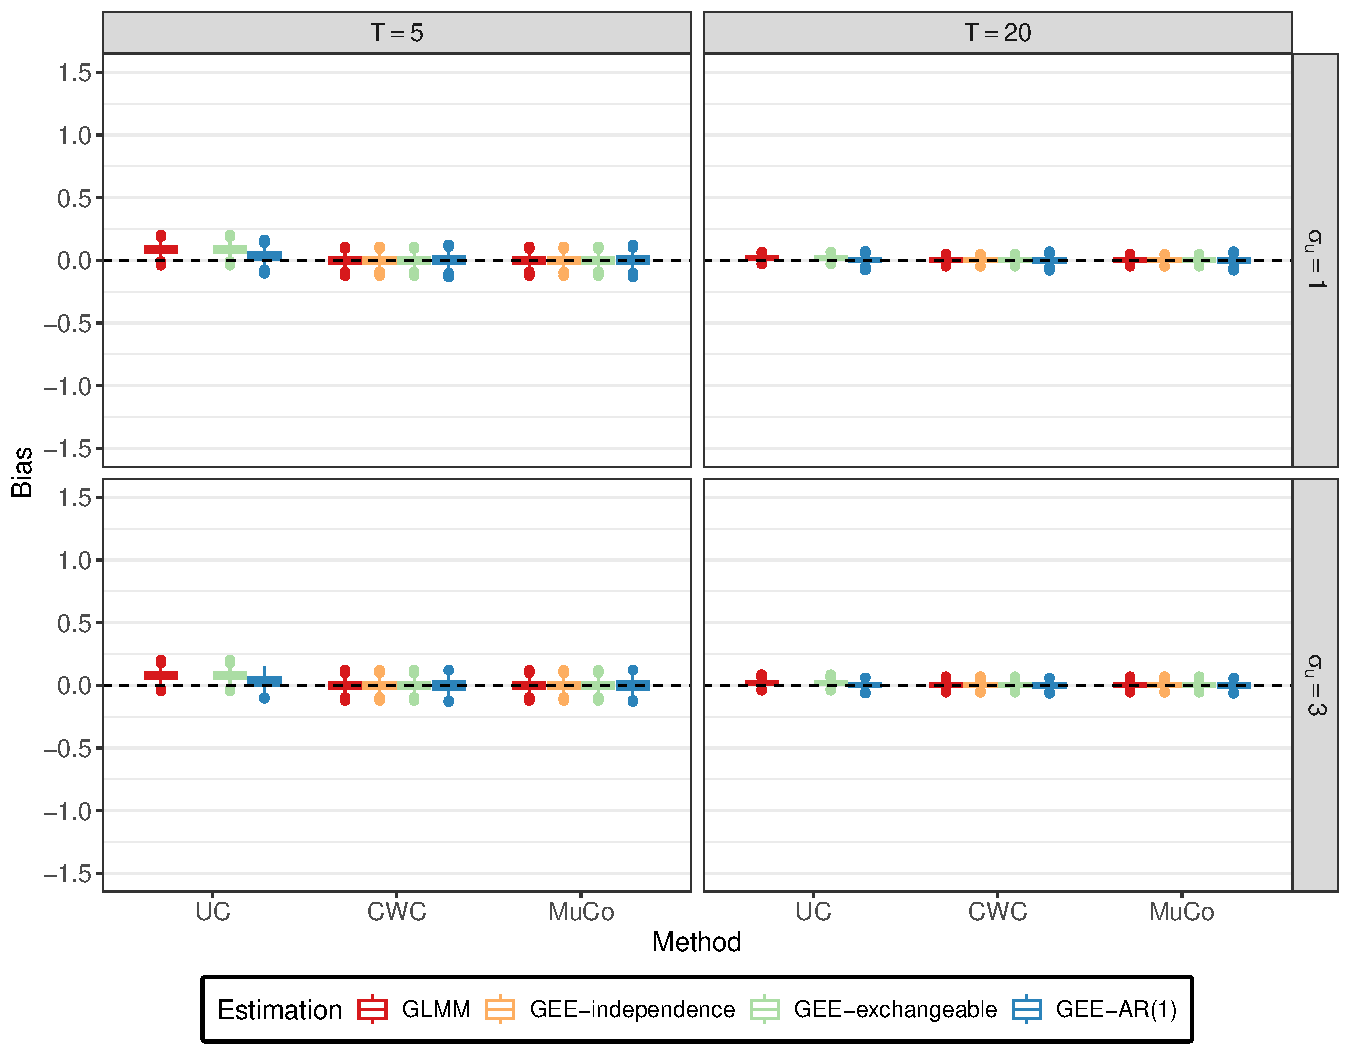
\includegraphics[width=\linewidth, keepaspectratio]{Figures/pred_continuous_out_continuous_bias_plot_T_total-vs-sd.u0_within.pdf}
%         \caption{Within-Person Effect}\label{fig:dgm1-within}
%     \end{subfigure}
%     \hfill
%     \begin{subfigure}{0.49\linewidth}
%         \centering
%         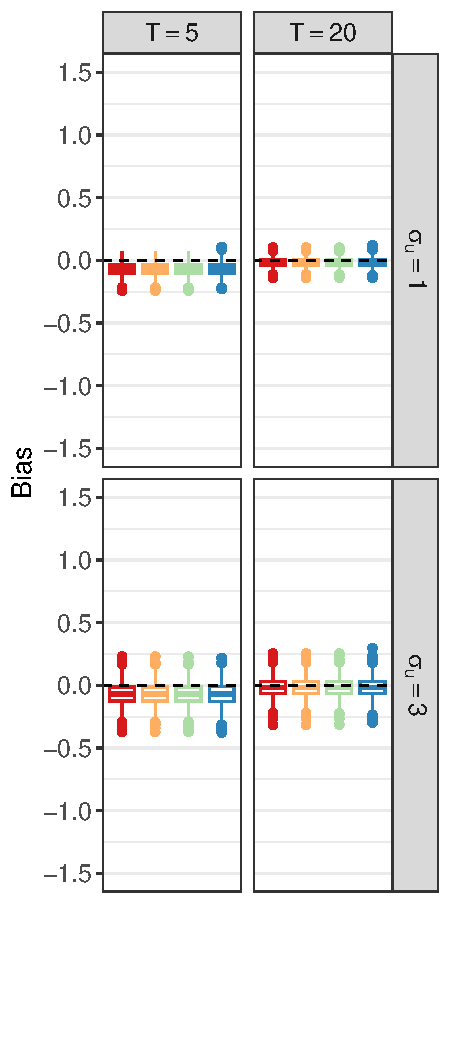
\includegraphics[height=6, keepaspectratio]{Figures/pred_continuous_out_continuous_bias_plot_T_total-vs-sd.u0_contextual.pdf}
%         \caption{Contextual Effect (Method 3)}\label{fig:dgm1-contextual}
%     \end{subfigure}
%     \label{fig:dgm1}
%     % \begin{figurenote}
%     %     \ldots
%     % \end{figurenote}
% \end{center}

\begin{center}
    \captionof{figure}{Bias for DGM 1 in Within-Person and Contextual Effect for Different Estimation Approaches}
     \hspace*{-1.5cm}
    \begin{subfigure}{0.80\linewidth}  % Set width proportionally for the first figure
        \centering
        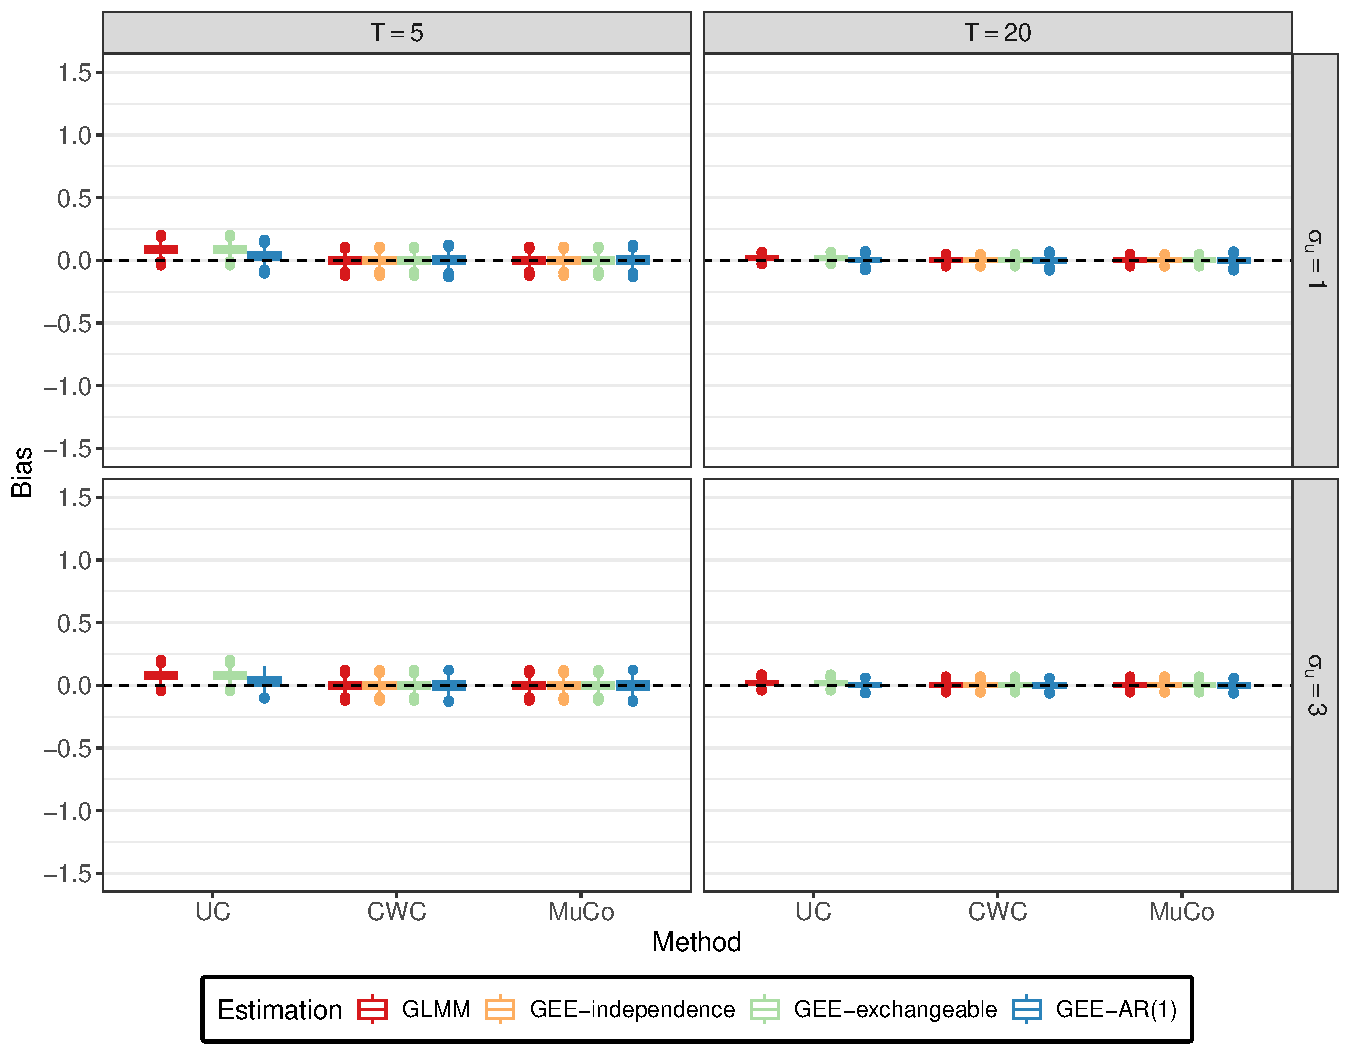
\includegraphics[height=10.6cm, keepaspectratio]{Figures/pred_continuous_out_continuous_bias_plot_T_total-vs-sd.u0_within.pdf}
        \caption{Within-Person Effect $\beta_1$}\label{fig:dgm1-within}
    \end{subfigure}
    \hfill
    \begin{subfigure}{0.25\linewidth}  % Set width proportionally for the second figure
        \centering
        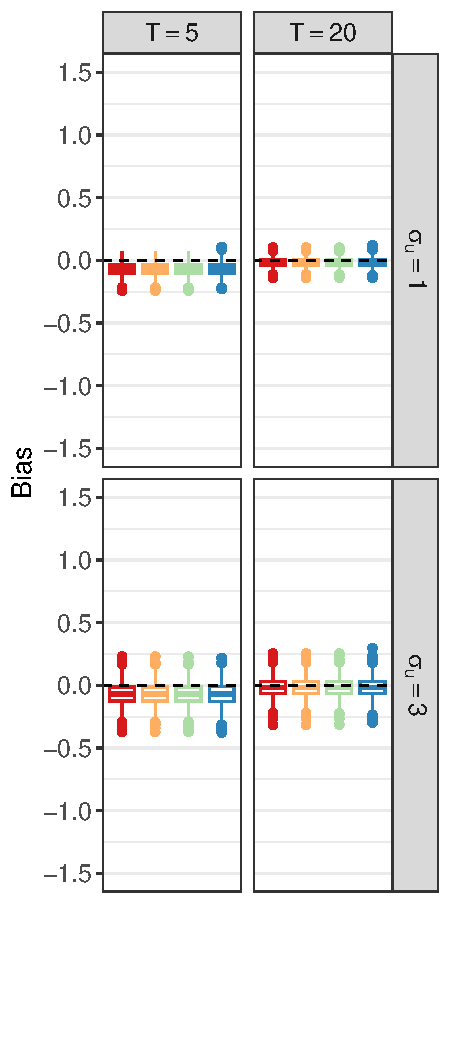
\includegraphics[height=10.6cm, keepaspectratio]{Figures/pred_continuous_out_continuous_bias_plot_T_total-vs-sd.u0_contextual.pdf}
        \caption{Contextual Effect $\gamma_{01}$ (Method MuCo)}\label{fig:dgm1-contextual}
    \end{subfigure}
    \label{fig:dgm1}
    \begin{flushleft}
        \begin{figurenote}
        The boxplot shows bias based on 1000 replications for data-generating model 1, which includes a continuous predictor and outcome. The boxes represent the interquartile range (IQR) from the 25th to 75th percentiles, with the median indicated by the horizontal line inside. Whiskers extend to 1.5 times the IQR, and replications outside this range are plotted as dots. UC = uncentered, CWC = centered within clusters, MuCo = Mundlak contextual, GLMM = generalized linear mixed model, GEE = generalized estimating equations. $T$ represents the total number of time points, and $\sigma_u$ denotes the random intercept residual variance. Y-axis breaks represent large intervals relative to bias but are consistent across data-generating models. In panel (a), GEE-UC with an independence correlation structure falls outside the plotted range, with estimates tightly clustered around 2.7 across all four scenarios.

        % The boxplot shows bias based on 1000 replications for data-generating model 1, which includes a continuous predictor and outcome. The boxes represent the interquartile range from the 25th to 75th percentiles, with the median indicated by the horizontal line inside. Whiskers extend to 1.5 times the IQR, and replications outside this range are plotted as dots. UC refers to uncentered, CWC to centered within clusters, and MuCo to Mundlak contextual, GLMM to generalized linear mixed model, GEE to generalized estimating equations. $T$ represents the total number of time points, and $\sigma_u$ denotes the random intercept residual variance. Y-axis breaks represent large intervals relative to bias but were chosen to be consistent across data-generating models. In panel (a), GEE-UC with independence correlation structure falls outside the plotted range, with estimates clustered tightly around 2.7 across all four scenarios.
        
        % Bias is shown for for data-generating model 1, which includes a continuous predictor and outcome. UC = uncentered; CWC = centered within clusters; MuCo = Mundlak contextual; $T$ = total number of time points; $\sigma_u$ = random intercept variance. Y-axis breaks represent large intervals relative to bias but were chosen to be consistent across data-generating models. In panel (a), GEE-UC with independence correlation structure falls outside the plotted range, with estimates clustered tightly around 2.7 across all four scenarios.
        
        % UC: Uncentered, CWC: centered within clusters, MuCo: Mundlak Contextual, T: total number of timepoints, $\sigma_u$: the random intercept residual variance. The breaks on the $Y$-axis represent large steps relative to bias, but were chosen to be consistent with the other DGMs. For panel (a), GEE-UC-independence fell outside the bounds, but has estimates tightly clustered around 2.7 (for all four scenarios).
    \end{figurenote}
    \end{flushleft}
\end{center}

% \begin{center}
%     \captionof{figure}{Bias for DGM 1 in Within-Person and Contextual Effect for Different Estimation Approaches}
%     \begin{subfigure}{1.1\linewidth}
%         \centering
%         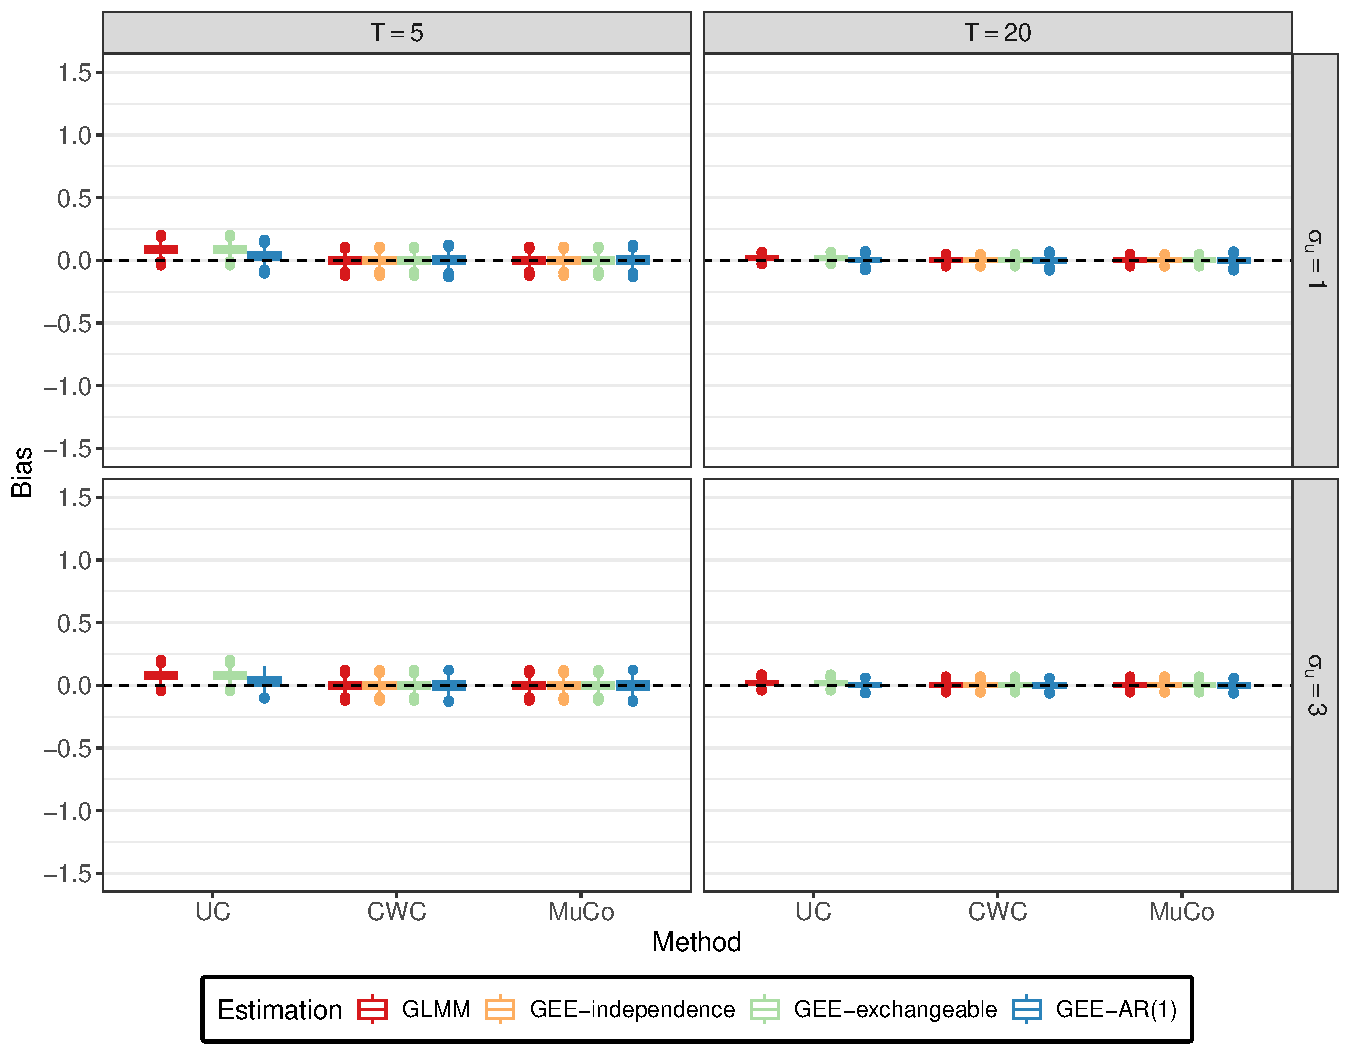
\includegraphics[width=\linewidth, keepaspectratio]{Figures/pred_continuous_out_continuous_bias_plot_T_total-vs-sd.u0_within.pdf}
%         \caption{Within-Person Effect}\label{fig:dgm1-within}
%     \end{subfigure}
%     \begin{subfigure}{1.1\linewidth}
%         \centering
%         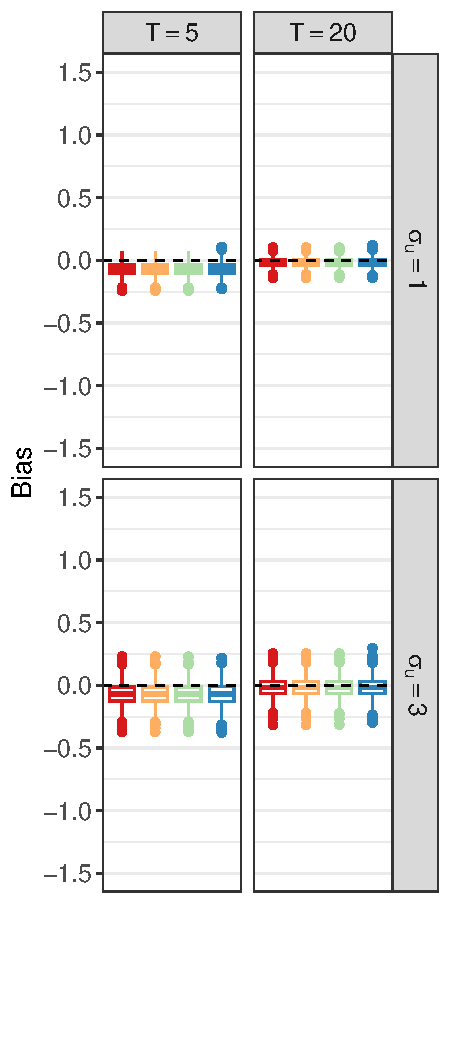
\includegraphics[width=\linewidth, keepaspectratio]{Figures/pred_continuous_out_continuous_bias_plot_T_total-vs-sd.u0_contextual.pdf}
%         \caption{Contextual Effect (Method 3)}\label{fig:dgm1-contextual}
%     \end{subfigure}
%     \label{fig:dgm1}
%     % \begin{figurenote}
%     %     \ldots
%     % \end{figurenote}
% \end{center}

\newpage

% \begin{center}
%     \captionof{figure}{Bias for DGM 2 in Within-Person and Contextual Effect for Different Estimation Approaches}
%     \begin{subfigure}{1.1\linewidth}
%         \centering
%         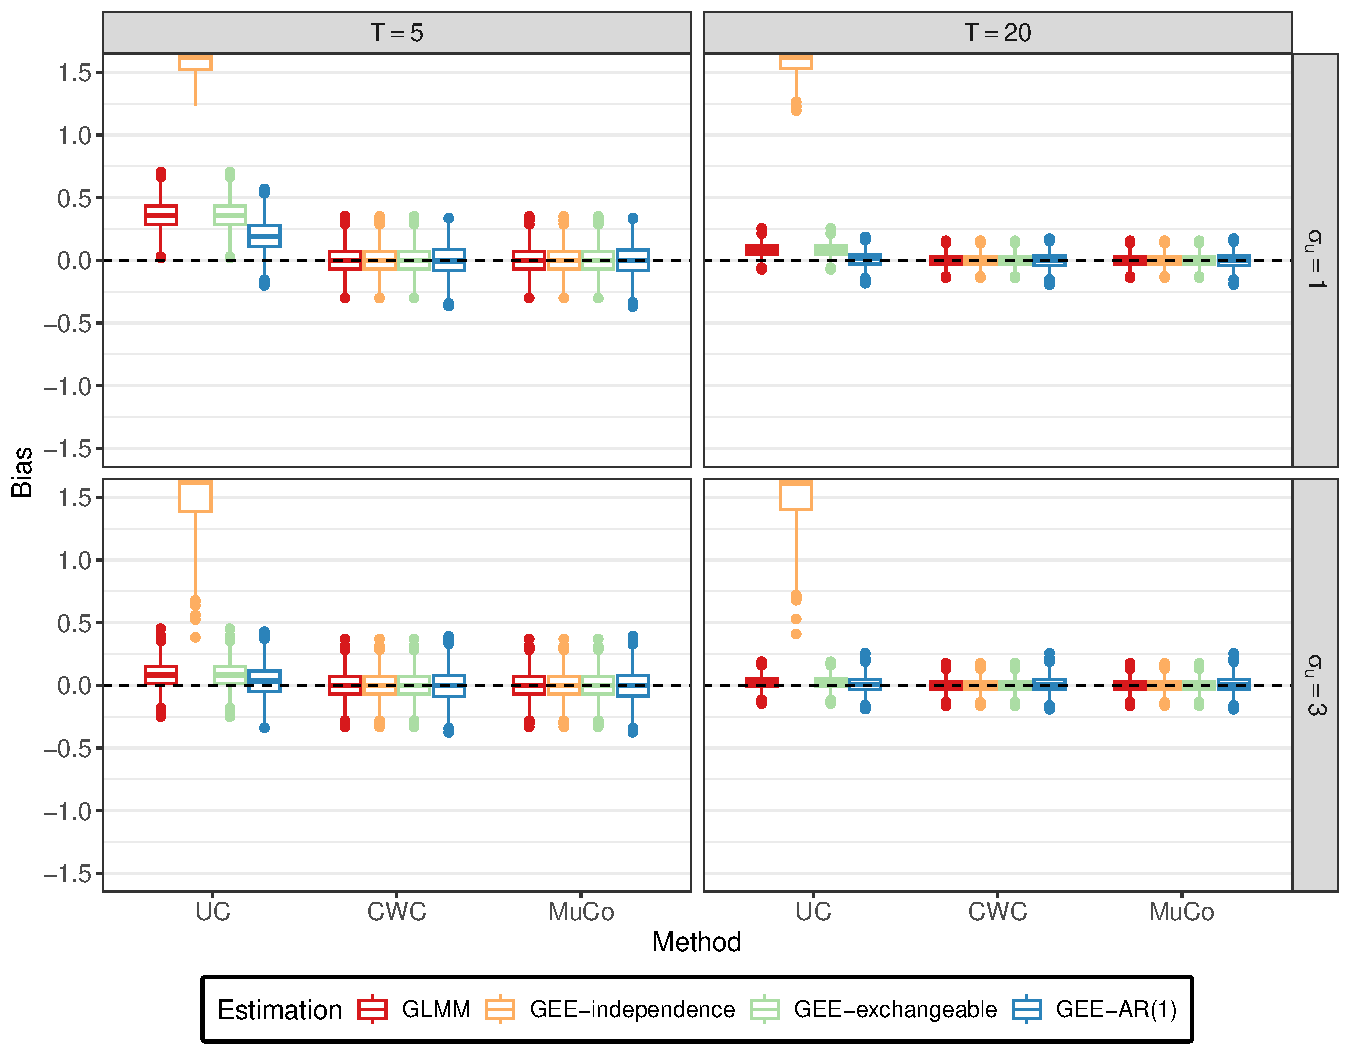
\includegraphics[width=\linewidth, keepaspectratio]{Figures/pred_binary_out_continuous_bias_plot_T_total-vs-sd.u0_within.pdf}
%         \caption{Within-Person Effect}\label{fig:dgm2-within}
%     \end{subfigure}
%     % \hfill
%     \begin{subfigure}{1.1\linewidth}
%         \centering
%         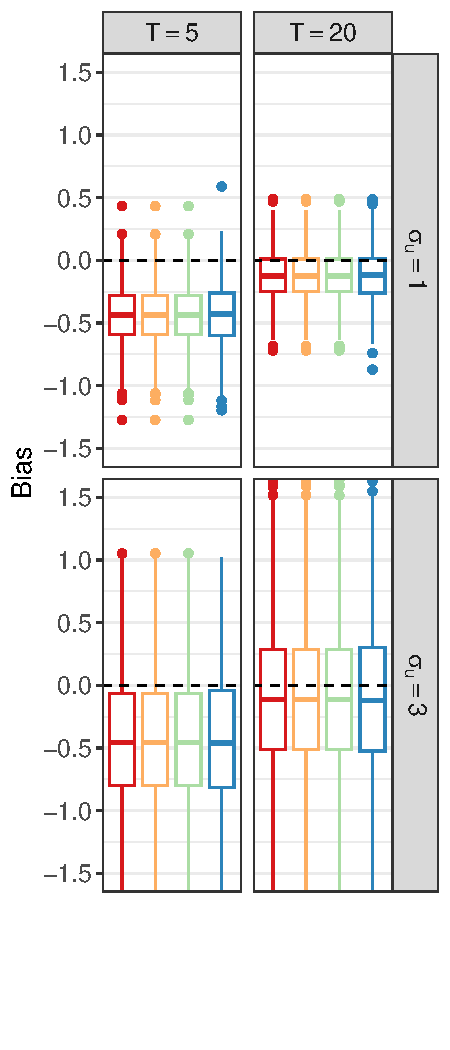
\includegraphics[width=\linewidth, keepaspectratio]{Figures/pred_binary_out_continuous_bias_plot_T_total-vs-sd.u0_contextual.pdf}
%         \caption{Contextual Effect (Method 3)}\label{fig:dgm2-contextual}
%     \end{subfigure}
%     \label{fig:dgm2}
%     % \begin{figurenote}
%     %     \ldots
%     % \end{figurenote}
% \end{center}


\begin{center}
    \captionof{figure}{Bias for DGM 2 in Within-Person and Contextual Effect for Different Estimation Approaches}
     \hspace*{-1.5cm}
    \begin{subfigure}{0.80\linewidth}  % Set width proportionally for the first figure
        \centering
        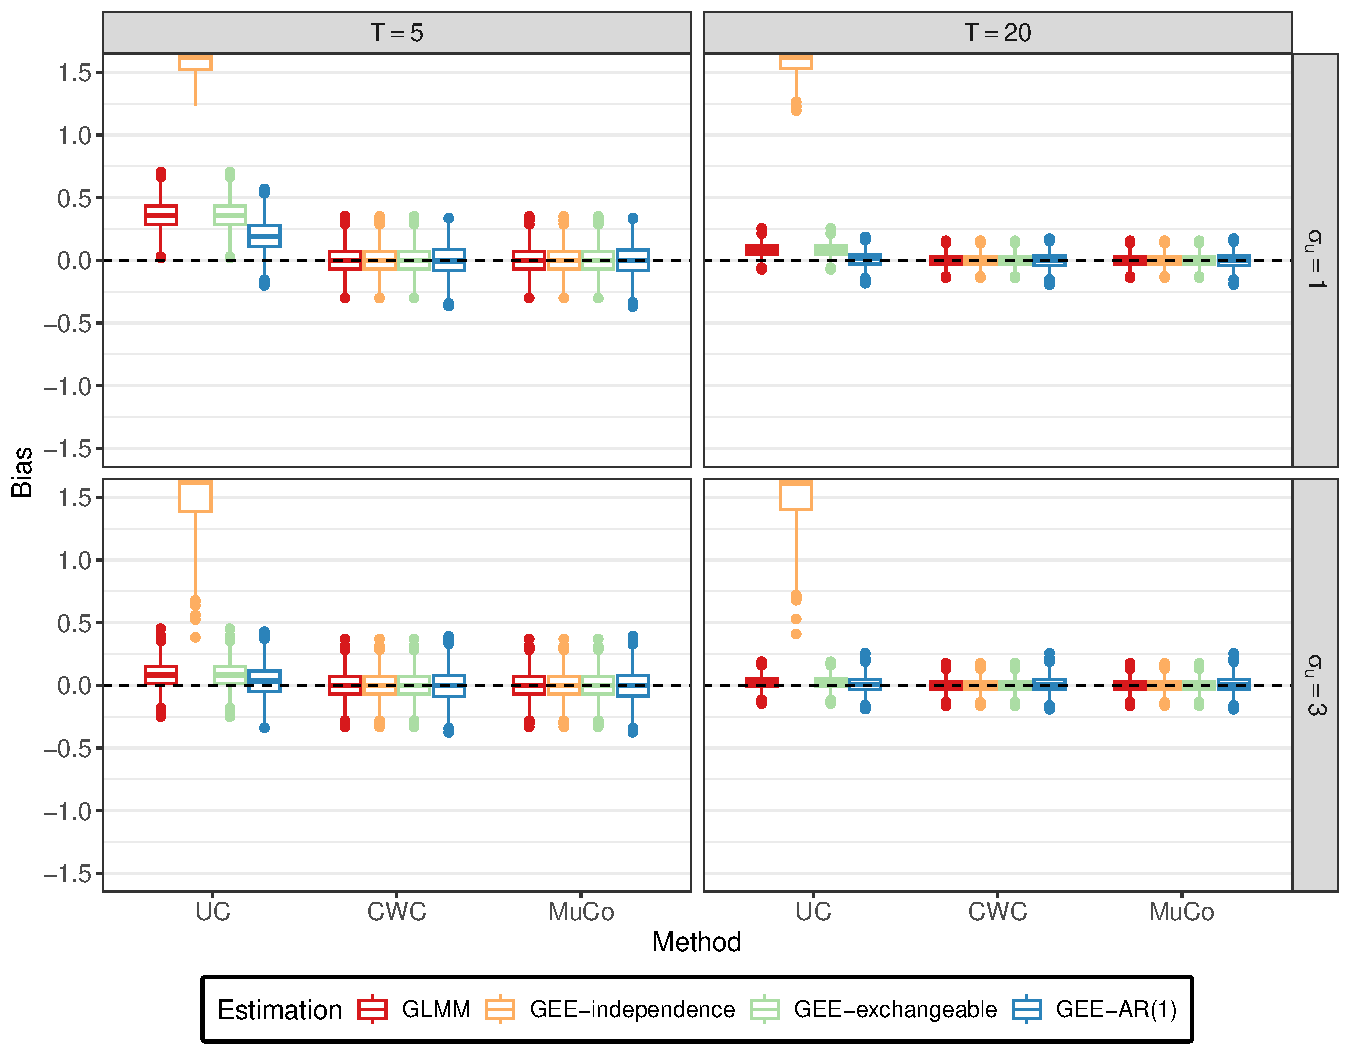
\includegraphics[height=10.6cm, keepaspectratio]{Figures/pred_binary_out_continuous_bias_plot_T_total-vs-sd.u0_within.pdf}
        \caption{Within-Person Effect $\beta_1$}\label{fig:dgm2-within}
    \end{subfigure}
    \hfill
    \begin{subfigure}{0.25\linewidth}  % Set width proportionally for the second figure
        \centering
        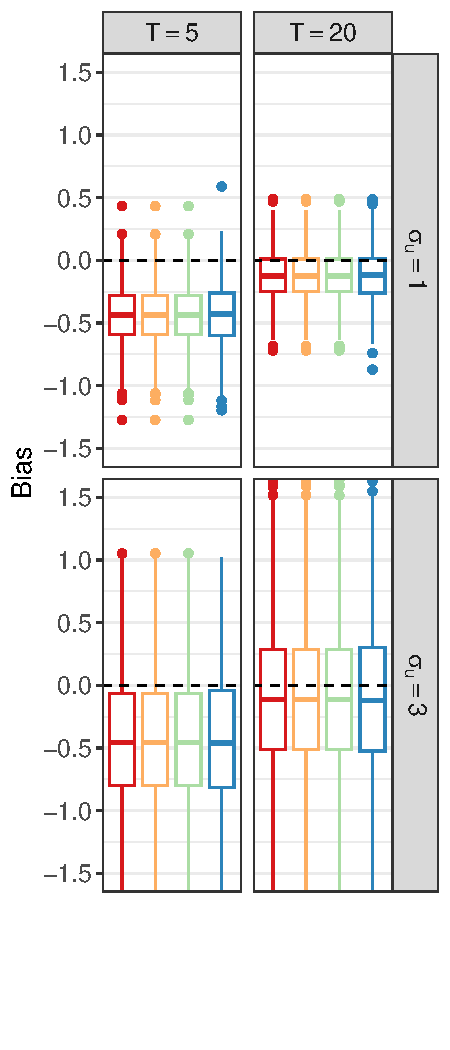
\includegraphics[height=10.6cm, keepaspectratio]{Figures/pred_binary_out_continuous_bias_plot_T_total-vs-sd.u0_contextual.pdf}
        \caption{Contextual Effect $\gamma_{01}$ (Method MuCo)}\label{fig:dgm2-contextual}
    \end{subfigure}
    \label{fig:dgm2}
    \begin{flushleft}
        \begin{figurenote}
        The boxplot shows bias based on 1000 replications for data-generating model 2, which includes a binary predictor and continuous outcome. The boxes represent the interquartile range (IQR) from the 25th to 75th percentiles, with the median indicated by the horizontal line inside. Whiskers extend to 1.5 times the IQR, and replications outside this range are plotted as dots. UC = uncentered, CWC = centered within clusters, MuCo = Mundlak contextual, GLMM = generalized linear mixed model, GEE = generalized estimating equations. $T$ represents the total number of time points, and $\sigma_u$ denotes the random intercept residual variance.

        
        % The boxplot shows bias based on 1000 replications for data-generating model 2, which includes a binary predictor and continuous outcome. The boxes represent the interquartile range from the 25th to 75th percentiles, with the median indicated by the horizontal line inside. Whiskers extend to 1.5 times the IQR, and points outside this range are considered outliers, plotted as dots. UC refers to uncentered, CWC to centered within clusters, and MuCo to Mundlak contextual. $T$ represents the total number of time points, and $\sigma_u$ denotes the random intercept residual variance.
        % Bias is shown for data-generating model 2, which includes a binary predictor and continuous outcome. UC refers to uncentered, CWC to centered within clusters, and MuCo to Mundlak contextual. $T$ represents the total number of time points, and $\sigma_u$ denotes the random intercept residual variance.
    \end{figurenote}
    \end{flushleft}
\end{center}

\paragraph{DGM 3: Continuous Predictor and Binary Outcome}

Figure~\ref{fig:dgm3} shows the results for DGM 3. While higher \(T\) again reduced variability, patterns diverged from those in DGMs with continuous outcomes. Method UC showed increasing bias in GEEs models as \(\sigma_u\) increased under exchangeable and AR(1) structures and an opposite trend under the independence structure. Notably, disaggregation performance varied across methods: CWC estimates were more biased than MuCo estimates across estimation approaches. More specifically, GLMM-CWC yielded biased within-person estimates even under optimal conditions ($T = 20$), whereas GLMM-MuCo yielded no bias under these circumstances. GEEs were biased for both disaggregation methods (GEE-CWC and GEE-MuCo), even under optimal conditions ($T = 20$ and $\sigma_u = 1$), though GEE-MuCo showed comparatively smaller bias. For contextual effects estimated by method MuCo, GLMM was clearly superior to GEEs across all conditions, especially when \(\sigma_u \) was large. As DGM 1, the contextual effects of GLMM where unbiased under a large number of timepoints, suggesting that scenarios with continuous predictors tend to be unbiased. These findings suggest that in logistic models, GEEs struggles to recover both within-person and contextual effects. Furthermore, within GLMM, Method MuCo is essential to avoid bias in the within-person effect.

\paragraph{DGM 4: Binary Predictor and Outcome}

Figure~\ref{fig:dgm4} displays the results for DGM 4. Patterns were similar to DGM 3, reflecting the shared binary outcome. Method UC produced biased within-person estimates in all models, with the exception of GEE-independence under high unexplained heterogeneity (\(\sigma_u = 3\))—a result that is difficult to explain. Unlike DGM 3,  in the shown scenarios GLMM-CWC performed comparably well as GLMM-MuCo. However, across all scenarios, MuCo still outperformed CWC with a maximum bias of 0.07 and 0.13 respectively. As in DGM 3, all GEEs implementations with methods CWC and MuCo yielded biased results. However, unlike DGM 3, when unexplained heterogeneity was high, CWC and MuCo yielded similar estimates. For the contextual effect estimated by the MuCo method, GLMM consistently outperformed GEEs, where bias in GEEs increased as \(\sigma_u\) increased. As DGM 2, the contextual effects of GLMM where biased under a large number of timepoints, suggesting that scenarios with binary predictors tend to be biased. Overall, GLMM-MuCo was again the most consistent and robust method across conditions.

\input{Figures/results-dgm3-boxplots}

\newpage

% \begin{center}
%     \captionof{figure}{Bias for DGM 4 in Within-Person and Contextual Effect for Different Estimation Approaches}
%     \begin{subfigure}{1.1\linewidth}
%         \centering
%         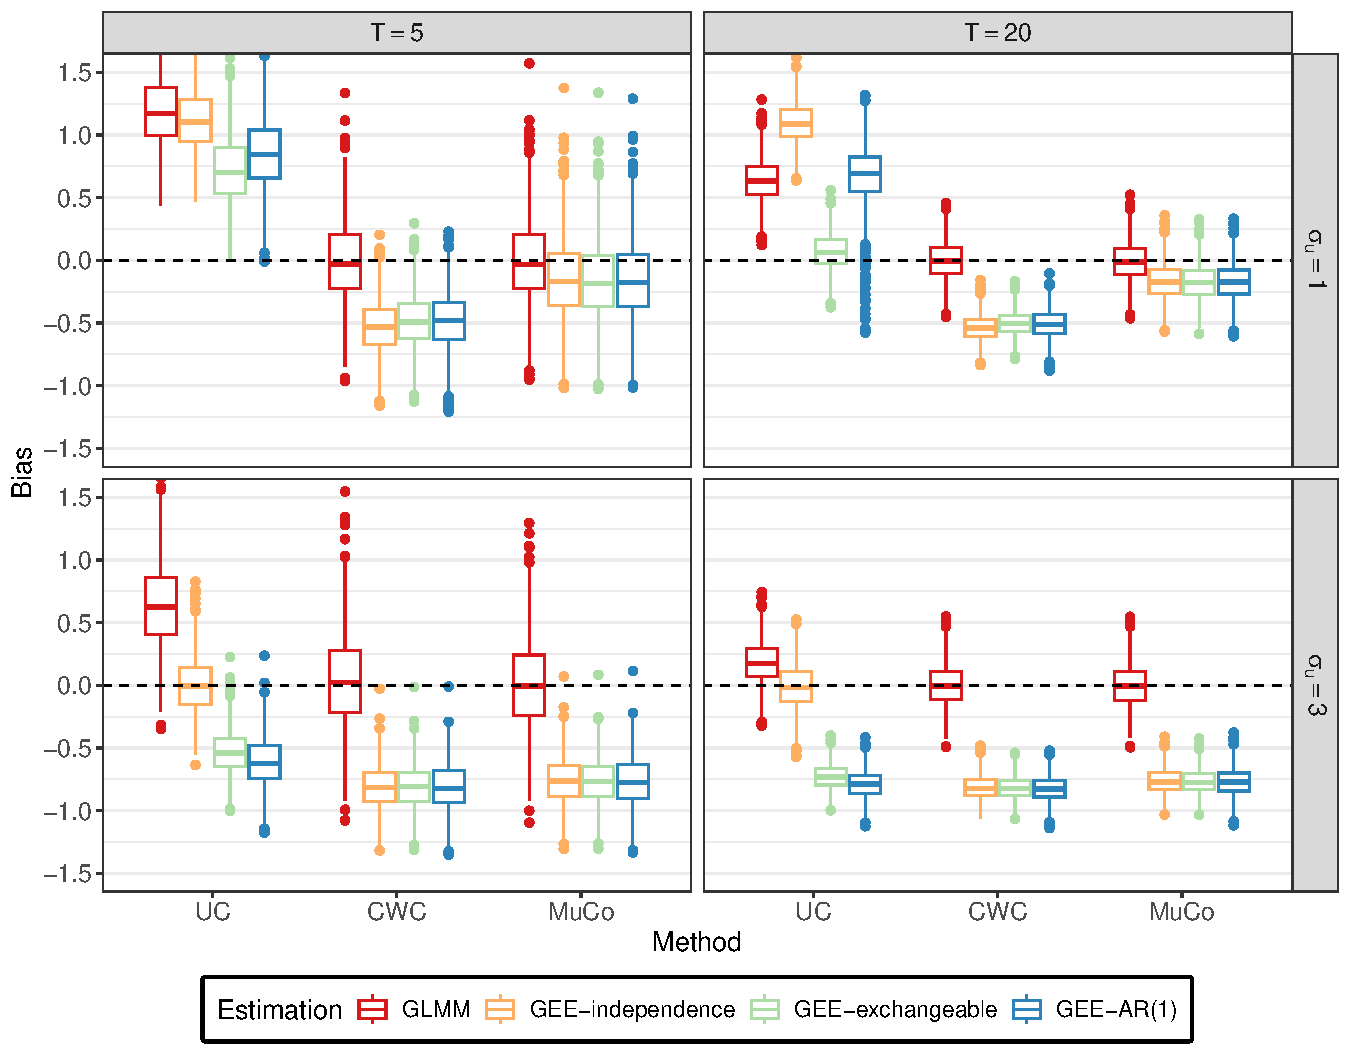
\includegraphics[width=\linewidth, keepaspectratio]{Figures/pred_binary_out_binary_bias_plot_T_total-vs-sd.u0_within.pdf}
%         \caption{Within-Person Effect}\label{fig:dgm4-within}
%     \end{subfigure}
%     % \hfill
%     \begin{subfigure}{1.1\linewidth}
%         \centering
%         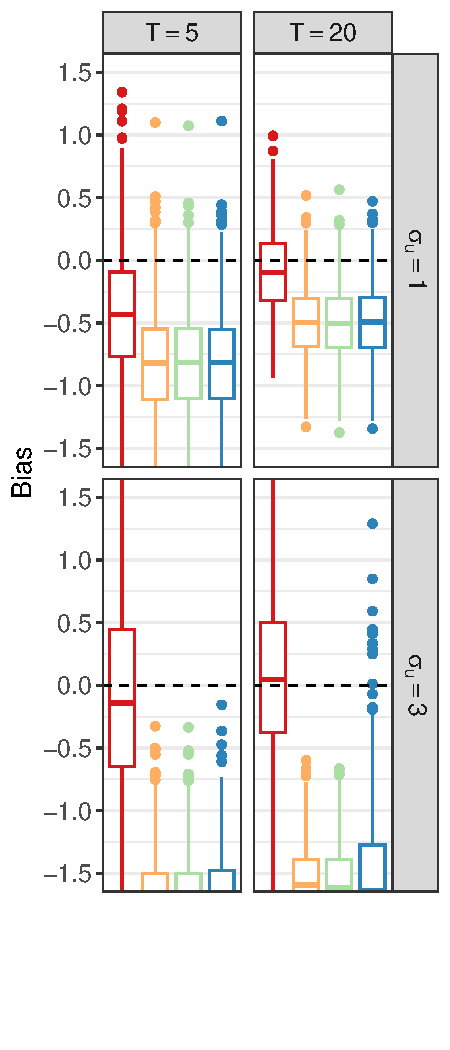
\includegraphics[width=\linewidth, keepaspectratio]{Figures/pred_binary_out_binary_bias_plot_T_total-vs-sd.u0_contextual.pdf}
%         \caption{Contextual Effect for Mundlak's Contextual Model}\label{fig:dgm4-contextual}
%     \end{subfigure}
%     \label{fig:dgm4}
%     \begin{figurenote}
%         UC = uncentered predictor, CWC = centered within clusters predictor, MuCo = Mundlak's contextual model.
%     \end{figurenote}
% \end{center}


\begin{center}
    \captionof{figure}{Bias for DGM 4 in Within-Person and Contextual Effect for Different Estimation Approaches}
     \hspace*{-1.5cm}
    \begin{subfigure}{0.80\linewidth}  % Set width proportionally for the first figure
        \centering
        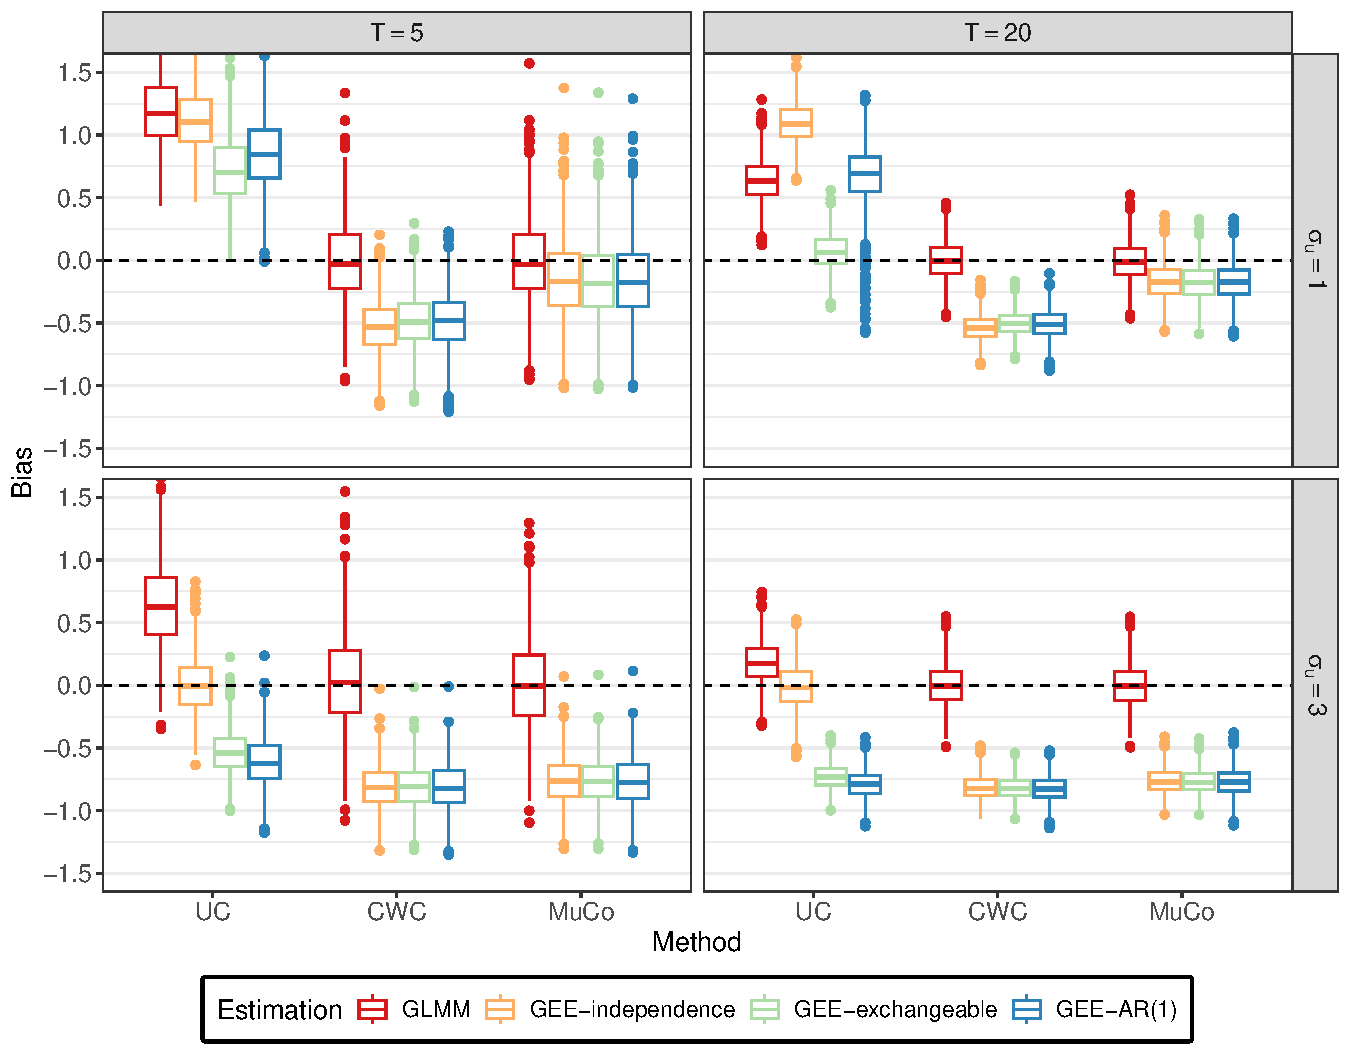
\includegraphics[height=10.6cm, keepaspectratio]{Figures/pred_binary_out_binary_bias_plot_T_total-vs-sd.u0_within.pdf}
        \caption{Within-Person Effect $\beta_1$}\label{fig:dgm4-within}
    \end{subfigure}
    \hfill
    \begin{subfigure}{0.25\linewidth}  % Set width proportionally for the second figure
        \centering
        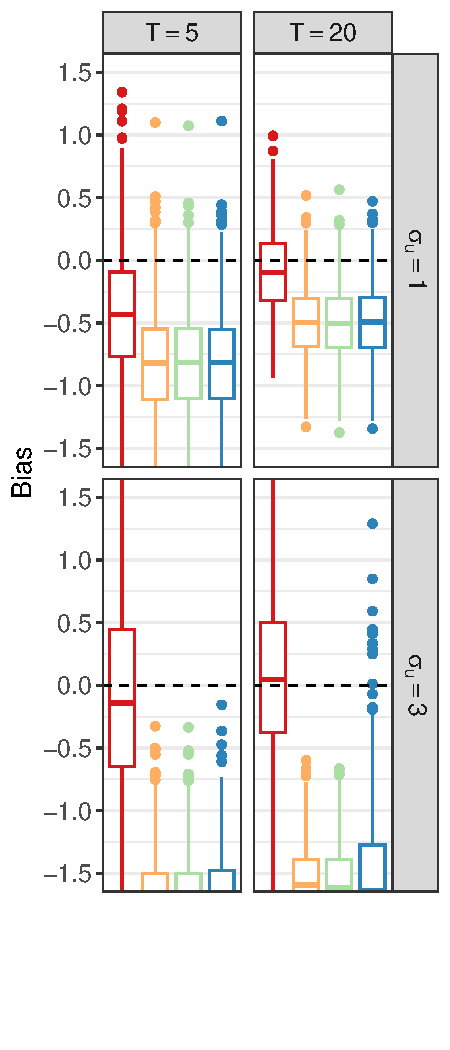
\includegraphics[height=10.6cm, keepaspectratio]{Figures/pred_binary_out_binary_bias_plot_T_total-vs-sd.u0_contextual.pdf}
        \caption{Contextual Effect $\gamma_{01}$ (Method MuCo)}\label{fig:dgm4-contextual}
    \end{subfigure}
    \label{fig:dgm4}
    \begin{flushleft}
        \begin{figurenote}
        The boxplot shows bias based on 1000 replications for data-generating model 4, which includes a binary predictor and outcome. The boxes represent the interquartile range (IQR) from the 25th to 75th percentiles, with the median indicated by the horizontal line inside. Whiskers extend to 1.5 times the IQR, and replications outside this range are plotted as dots. UC = uncentered, CWC = centered within clusters, MuCo = Mundlak contextual, GLMM = generalized linear mixed model, GEE = generalized estimating equations. $T$ represents the total number of time points, and $\sigma_u$ denotes the random intercept residual variance.

        
        % The boxplot shows bias based on 1000 replications for data-generating model 4, which includes a binary predictor and outcome. The boxes represent the interquartile range from the 25th to 75th percentiles, with the median indicated by the horizontal line inside. Whiskers extend to 1.5 times the IQR, and points outside this range are considered outliers, plotted as dots. UC refers to uncentered, CWC to centered within clusters, and MuCo to Mundlak contextual. $T$ represents the total number of time points, and $\sigma_u$ denotes the random intercept residual variance.
        % UC = Uncentered, CWC = centered within clusters, MuCo = Mundlak Contextual. 
    \end{figurenote}
    \end{flushleft}
\end{center}

\newpage
\section{Discussion}

% \subsection{Summary and Contribution}  
% This study addressed an important gap in the literature on clustered longitudinal data analysis by extending the within- and between-person effects debate from the MLM framework to GLMMs and GEEs with different variable types. First, we have extended the well-known discussion about within-person versus between-person slopes from the MLM literature focusing on continuous predictors and outcomes, to situations with a binary predictor and/or outcome. Second, we evaluated how well different disaggregation strategies within the context of GLMMs and GEEs recover the within-person effect and the contextual effect (i.e., the difference...) depending on combinations of predictor and outcome types. Although prior work has examined binary predictors in MLMs and binary outcomes in GLMMs, and some studies have compared estimation frameworks across disciplines, no study has brought these strands together. This article fills that gap by offering a systematic evaluation of disaggregation methods across estimation strategies and data types. 

This study addressed an important gap in the literature on clustered longitudinal data analysis by extending the well-known within- and between-person effects debate beyond the MLM framework to GLMMs and GEEs with different variable types. First, we generalized the established distinction between within- and between-person slopes—traditionally discussed for continuous variables—to settings involving binary predictors and/or outcomes. Second, we evaluated how well each disaggregation method, implemented in GLMMs and GEEs, recovered the within-person effect and contextual effect (i.e., the difference between the between- and within-person slopes). To assess the role of variable scale, analyses were conducted across combinations of binary and continuous predictor and outcomes. Although prior work has examined binary predictors in MLMs and binary outcomes in GLMMs, and some studies have compared estimation frameworks across disciplines, no study has brought these strands together. This article fills that gap by offering a systematic evaluation of disaggregation methods across estimation strategies and data types. 

% First, we have extended the well-known discussion about within-person versus between-person slopes from the MLM literature focusing on continuous predictors and outcomes, to situations with a binary predictor and/or outcome. Second, we evaluated how well different disaggregation strategies within the context of GLMMs and GEEs recover the within-person effect and the contextual effect (i.e., the difference...) depending on combinations of predictor and outcome types. 

% , no study to date has systematically investigated (a) how disaggregation methods applied to GLMM perform in the presence of binary as opposed to continuous variables, nor (b) how contextual effects should be modeled in GEEs. This article fills that gap by offering a comprehensive evaluation of disaggregation method across frameworks and data types.

\subsection{Main Findings}

% Simulation results revealed that, for the specific scenarios investigated in this study, GLMM with Mundlak's contextual model yielded the most robust results across variable types. Surprisingly, the GLMM with person-mean centering (method CWC)

The simulation results demonstrate that the effectiveness of disaggregation methods depends on both the estimation framework and the type of variables involved. As expected, when contextual effects were present, the uncentered predictor approach consistently failed to recover the within-person effect, both in the GLMM and across all three GEE variants. This failure was particularly pronounced for scenarios involving (a) a small number of time points and (b) binary predictors or outcomes, where bias and variability were substantially larger than in continuous-variable settings. Furthermore, with continuous outcomes (DGMs 1 and 2), all three disaggregation methods (CWC, HB, MuCo) performed comparably well across the GLMM and GEE variants. However, this pattern did not generalize to binary outcomes (DGMs 3 and 4). None of the GEE variants consistently recovered the within-person or contextual effects. In the GLMM context, the hybrid or Mundlak methods produced robust estimates, whereas the CWC approach was more susceptible to bias—especially with continuous predictors. When comparing results across predictor types, we found that GLMM estimates of the contextual effect were more biased for binary predictors (DGMs 2 and 4) than for continuous predictors (DGMs 1 and 3). Taken together, these results point to consistent differences in performance across methods, designs and variable types.

% \subsection{Implications}

%  \begin{enumerate}
%      \item This pronounced bias in the binary variable setting underscore the heightened importance of applying a proper disaggregation method, especially in models involving binary data.
%      \item The ability of GEEs to retrieve the effects under all disaggregation strategies (CWC, HB, MuCo) suggests that in such settings, GEEs may serve as a viable alternative to GLMMs for estimating both within-person and contextual effects.
%      \item The suboptimal performance of GLMM with CWC in the binary outcome settings suggest that even well-established centering approaches can behave unexpectedly, emphasizing the need for careful methodological choices in applied research. 
%      \item The contextual effect is more biased under binary predictors (see \parencite[]{asparouhov_latent_2019})
%      \item 
%  \end{enumerate}

% \paragraph{Implication 1}

These findings yield several insights. First, although the person-mean centered-only approach (Method CWC) is often treated as the default or even “gold standard” for estimating within-person effects in multilevel modeling \parencite[e.g.,][]{hamaker_fixed_2020, enders_centering_2007, raudenbush_adaptive_2009}, our results indicate that this strategy may yield biased estimates when applied to binary outcomes. This is particularly concerning given the widespread use of this method in studies with continuous outcomes, where researchers may be inclined to extend the same approach to non-continuous settings. Our findings suggest that such a transfer is not without risk. To mitigate bias, we found that it is crucial to include the person-mean of the predictor as a predictor of the random intercept, as is done in Mundlak's contextual and the hybrid method. This discrepancy must stem from differences in the statistical properties of the identity and logit link functions. Specifically, \textcite[p. 807]{neuhaus_geometric_1993} demonstrated that omitting relevant predictors in logistic models can lead to substantial bias in the estimated coefficients, even when the omitted variables are independent from those included. In the CWC formulation, the person-mean is omitted from the model, thereby violating this condition and potentially introducing bias.

% \paragraph{Implication 2}

Second, our findings contribute to the ongoing debate on the interpretability of GEEs by clarifying a key point of contention. In line with earlier work \parencite{begg_separation_2003}, we demonstrate that for continuous outcomes, GEEs—when paired with a disaggregation approach—yield estimates of within-person and contextual effects that closely mirror those from GLMMs. This equivalence is not incidental but follows directly from statistical theory: With an identity link and normally distributed outcomes, marginal (GEE) and conditional (GLMM) estimators coincide \parencite{zeger_models_1988, neuhaus_comparison_1991}. Yet, in psychological treatments, GEEs are often characterized as producing population-averaged estimates that preclude person-specific interpretations \parencite[e.g.,][]{mcneish_unnecessary_2017, ballinger_using_2004, bauer_fitting_2011}. However, it should be nuanced that with continuous outcomes, individual-level interpretations remain valid, allowing for the estimation of within-person parameters. 

The picture changes substantially for binary outcomes. Our simulations show that GEEs, even when combined with a disaggregation approach, cannot recover the true within-person and contextual effects. The degree of bias increases with the residual variance of the random intercept, aligning with prior work demonstrating that non-linear link functions—such as the logistic link—break the equivalence between GLMM and GEE estimates \parencite{neuhaus_comparison_1991, zeger_models_1988}. This divergence arises because the random intercept, which captures outcome heterogeneity due to unobserved covariates, is explicitly modeled in GLMMs but left unaccounted for in GEEs (For an illustration of the impact of the random intercept residual variance on this discrepancy, see \href{https://wardeiling.shinyapps.io/GLMM_population-averaged-and-person-specific-interpretations/}{wardeiling.shinyapps.io/GLMM\_population-averaged-and-person-specific-interpretations}). As a consequence, GEE estimates are attenuated toward zero \parencite{neuhaus_comparison_1991, zeger_models_1988}. This is visible in our results, where the GEE estimates fell consistently below the zero-bias line. In the context of positive true effects, this implies an underestimation of the effect magnitude. Accordingly, in the context of binary outcomes, \textcite[]{neuhaus_comparison_1991} pointed out that GEEs ``cannot provide estimates of changes within individuals over time; these are often quantities of central interest in longitudinal studies'' (p. 33). For research questions that focus on within-person processes, as is often the case in psychology, such attenuation renders the logit-linked GEE framework ill-suited. In these contexts, conditional models such as GLMMs are generally more appropriate \parencite[p. 78]{allison_logistic_1999}.

% \paragraph{Implication 3}

Third, our findings highlight limitations in estimating contextual effects when relying on observed person-means within the GLMM framework. Across most simulation conditions, we observed small but consistent bias in the contextual estimates. One plausible contributor is Lüdtke’s bias: the sample-based person-mean is an imperfect proxy for the true latent mean, especially when the number of observations per person is limited \parencite{ludtke_multilevel_2008}. In line with prior work on the limitations of disaggregation using observed means \parencite{asparouhov_latent_2019}, the magnitude of bias increased under stronger contextual effects, reduced between-person variance, and smaller cluster sizes. Notably, this bias was substantially more pronounced for binary predictors (DGMs 2 and 4) than for continuous ones (DGMs 1 and 3), underscoring the additional complexities introduced when modeling non-continuous predictors. While Lüdtke’s bias offers a partial explanation, other sources likely contribute as well. As discussed in the section on the MLM, binary predictors pose unique challenges such as truncated distributions and violations of independence \parencite[see also][]{asparouhov_latent_2019}. In the DGMs, the binary predictor was conceptualized as the observed expression of a latent continuous construct. If this is the case, we recommend the use of latent centering approaches of multilevel structural equation modeling \parencite[e.g.,][]{asparouhov_latent_2019}, which provide more robust estimates, particularly in the presence of binary predictors.

% \paragraph{Implication 4}

Finally, an unanticipated but important finding concerns the instability of GEE estimation when disaggregation methods are applied. Although GEEs are frequently commended for their robustness to misspecification of the working correlation structure \parencite[e.g.,][]{zeger_models_1988, ballinger_using_2004}, our simulations revealed instances of extreme and erratic estimates under several conditions. These estimation anomalies were specific to binary outcomes and most prevalent when the AR(1) working correlation structure was used—rarely occurring under an exchangeable structure and absent under independence (see the Appendix for details). This suggests that the combination of a logit link with complex correlation structures, particularly when misspecified, may exacerbate numerical instability in GEEs.

\subsection{Limitations and Future Directions}

This study has several limitations that point to important directions for future research. First, our simulations examined the recoverability of within-person effects under DGMs that satisfy the core assumptions of GLMMs and GEEs \parencite[see][]{mcneish_unnecessary_2017}. In practice, however, these assumptions are often violated, potentially leading to biased estimates. Within biomedical applications, GEEs are sometimes preferred for their robustness to distributional assumptions about random effects \parencite{hubbard_gee_2010}, yet it remains unclear whether this robustness generalizes to the retrieval of within-person effects. Future studies should explicitly examine how violations—such as non-normal random effects or misspecified variance structures—impact estimation, and whether the equivalence of GEE and GLMM estimates for continuous outcomes persists under such conditions.

Second, while our focus was on random intercept models, the inclusion of random slopes is a central strength of the multilevel framework \parencite{bell_explaining_2015}. In longitudinal data, researchers are often interested in capturing within-person effects while allowing for individual differences in the strength of these effects \parencite[e.g.,][]{geschwind_mindfulness_2011}. Assuming a homogeneous within-person association across individuals can be overly restrictive, as many psychological processes plausibly vary from person to person. The inclusion of a random slope would alter the application of disaggregation methods in GLMM estimation, as the equivalence between the hybrid model and Mundlak’s contextual model is lost under this specification \parencite[]{snijders_multilevel_2011}. Additionally, since the GEE framework does not account for random slope heterogeneity, it remains an open question whether disaggregation-based GEEs can still recover within-person effects when such heterogeneity is present. Therefore, future research should extend the DGMs to include random slopes, allowing for a more comprehensive evaluation of GLMM methods and the suitability of GEE for investigating within-person effects in such contexts. 

Third, we restricted our simulations to binary predictors and outcomes. Although prior work has begun to explore centering strategies for multi-categorical predictors \parencite[e.g.,][]{yaremych_centering_2023}, applications involving multi-categorical outcomes remain largely unexamined. Expanding the current framework to accommodate these outcome types represents a critical step for broadening the generalizability of disaggregation methods.

\subsection{Conclusion}

Within the multilevel modeling literature, the importance of distinguishing within- from between-cluster effects has been stressed repeatedly and by many \parencite[e.g.,][]{enders_centering_2007, kreft_effect_1995, raudenbush_hierarchical_2002}, to the point that it has become standard practice among psychological researchers. However, the applicability of disaggregation methods to multilevel models with non-continuous predictors and outcomes, as well as GEEs, has not been systematically examined This study offers the first comprehensive account of how the within- and between-person effects debate extends to binary predictors, binary outcomes, and the GEEs framework. Based on our findings, we recommend using GLMMs with Mundlak’s contextual or the hybrid approach when estimating within-person effects regardless of variable type.

\printbibliography

\newpage
\appendix
\section{Handling of Extreme Parameter Estimates in GEEs}
\label{app:extremeGEEvalues}

Diagnostic evaluation of extreme parameter estimates is reported in the supplemental materials at \href{https://wardeiling.github.io/multilevel-vs-gee-binary/supplementary_materials.html}{wardeiling.github.io/multilevel-vs-gee-binary/supplementary\_materials.html}. This revealed that, when modeling binary outcomes, the \texttt{geeglm} function \parencite{halekoh_r_2006} occasionally produced bias estimates of implausibly large magnitude (e.g., $10^{12}$ or higher), likely reflecting non-convergence. Such extreme values consistently exceeded $\pm 10^{11}$, while the vast majority of estimates fell within a narrow range of $\pm 2.5$ units around the mean bias. Notably, the number of extreme estimates remained unchanged when using a threshold of $\pm 20$, $\pm 100$ or $\pm 10^{11}$, indicating that non-convergence resulted in extreme rather than moderate deviations from the true parameter values. Across 76 simulation scenarios, we observed at least one replication with an estimate exceeding $\pm 10^{11}$. Extreme estimates were specific to binary outcomes and most prevalent when the AR(1) working correlation structure was paired with a disaggregation method (methods CWC, HB and MuCo)—rarely occurring under an exchangeable structure and absent under independence. In one scenario, approximately half of the replications produced extreme values. To maintain the integrity of the reported results, we excluded all estimates exceeding $\pm 100$ from the final analyses. 

% \paragraph{Estimation of Within-Person Effects with Uncentered Predictor (L1/G1)}

% When predictors were uncentered (L1 for MLM, G1 for GEEs), as expected, we tended to find estimates that varied from the within-person effect when a contextual effect was present, variation across correlation structures and outcome type.

% % Model 1 (uncentered predictor only)

% For L1 models (uncentered predictor only), we found no bias when contextual effects were absent. However, under contextual effects, bias emerged and increased with larger between-person differences in $X$, larger contextual effects (for scenarios with continuous predictor and outcome the reverse was found), and fewer time points. Bias decreased with higher random intercept variance ($\sigma_u$), especially in continuous outcome settings, likely due to the increased proportion of unexplained to explained between-person variance in $\beta_{0i}$.

% For the G1 approaches with continuous outcomes, we found no bias for settings with no contextual effect as we did for the L1. For settings with contextual effect, we found that the exchangeable structure yielded practically indistinguishable results from L1, the AR(1) structure sometimes being closer to the within-effect and sometimes further away, and the independence structure consistenly being furthest away from the within-effect.

% For G1 models with binary outcomes, both the absence of contextual effects and unexplained heterogeneity ($\sigma_u = 0$) were required to eliminate bias, indicating greater sensitivity of binary outcomes to random effects. Under contextual effects, all G1 variants produced non-overlapping estimates, none of which consistently recovered the within-person effect.

% \paragraph{Estimation of Within-Person Effects With Parametrization Strategy}

% %%% Continuous outcome (MLM and GEEs)

% Scenarios with a continous outcome show correspondence of both modeling traditions, parametrization 2-4 and all working correlation structures. 

% %%% binary outcome

% With a binary outcome, both multilevel and GEEs approaches yielded estimates that differed from the DGMs under particular scenarios. 

% % Multilevel logistic model

% For GLMMs with binary outcomes (i.e., multilevel logistic model), we found in general that bias in the within-person effect (i.e., the difference between the specified within-person effect and the estimates) was absent or small when there were no between-person differences in X. However, bias increased with a smaller number of time points T and greater between-person variability in X. We also found that the L2 model (with only person-mean centered X) yielded consistently more biased results across scenarios compared to L3a and L4, the latter two yielded the same estimates. Only in the multilevel logistic model with continuous predictor, we found that the bias increased the size of the contextual effect increased.

% % GEEs general observations

% We found that the GEEs with binary outcomes (i.e. logit link) were in general not able to retrieve the specified within-person effect, with the exception of some scenarios that lacked unexplained heterogeneity in the outcome. The bias tended to be worse for situations with a continuous predictor. In line with the GLMM findings, we found that GEEs implementations (with continuous and binary predictors) with only person-mean centered X (G2) performed worse than the those including the cluster mean as predictor of the random intercept. However, within the strategies for including the predictor (G2, G3, G4), there was very little discrepancy in estimates across the implementations with different working correlation matrices.

% % GEEs specifically for predictor type

% For the continuous predictor setting, bias was found in the G3 and G4 implementations for all scenarios except those where no unexplained heterogeneity in Y was present ($\sigma_{u} = 0$) and the contextual effect was small ($\gamma_{01} = 0, 1$) or absent. G2 implementations did even worse, only being void of bias when there was no between-person variability in X, no contextual effect and no unexplained heterogeneity. For the binary predictor setting, bias was found in G3 and G4 implementations for all scenarios except those with unexplained heterogeneity ($\sigma_{u} = 1, 3$). G2 implementations again performed worse, also requiring the absence of a contextual effect, for bias to dissapear.

% \paragraph{Estimation of Contextual Effects}
% % General

% Across both modeling approaches and all implementations thereof we found substantial bias for most scenarios in the contextual effect (i.e., deviations from the specified contextual effect), with the bias generally being lower for the scenarios with continuous predictors as opposed to binary predictors. 

% % Multilevel Models

% For the multilevel implementations, we found across all four DGMs that the bias increased as the contextual effect got larger ($\gamma_{01} = 3$), the between-person variance in $X$ got smaller ($\sigma_{X,\text{b}} = 1$) and the number of time points $T$ decreased ($T = 5$; while being unrelated to $\sigma_{u}$ and $N$). When there was no contextual effect nor between-person variability in X, bias was absent from the DGMs with continuous outcome, and small for those with dichtomous outcomes (max 0.074). Although L3a and L4 generally yielded similar estimates across settings, for the settings with continuous predictor and binary outcome, L4 (Munlak's contextual model) tended to yield less bias.

% %%% GEEs

% %  GEEs identity link

% For the GEEs with identity link (continuous outcome), we found that the pattern of bias across all scenarios and parametrizations of predictor corresponded exactly to that of the MLM, with only minor discrepancies in estimates (neither performs better). 

% % GEEs logit link binary predictor

% For the GEEs with logit link (binary outcome), we found that the G4 parametrization performed better than the G3 parametrization. With a binary predictor, we found that findings of the G3 parametrization aligned with the GLMM when there was no unexplained heterogeneity ($\sigma_{u} = 0$), while yielding consistently greater bias for all other scenarios. On the other hand, the G4 parametrization generally aligned well with the GLMM, with the exception of (a) less bias (in exchangeable and independence structures) for scenarios with no contextual effect (g.01 = 0) and great unexplained heterogeneity (sd.u0 = 3), (b) greater bias for scenarios with non-zero random intercept variance (sd.u0 = 1 or 3) and non-zero contextual effect (g.01 = 1 or 3) and (c) implausible coefficient estimates for AR(1) structure.

% % GEEs logit link continuous predictor

% In the case of a continuous predictors, results of G3 only aligned with the GLMM findings when on top of no unexplained heterogeneity, the contextual effect was absent or small  ($\gamma_{01} = 0, 1$), yielding consistently greater bias for all other scenarios. On the other hand, the G4 parametrization aligned for some scenarios with the GLMM, but the GLMM performs better across the board than GEEs, with the exception of scenarios without contextual effect (g.01 = 0), where in particular GEEs performed well (the other two structures somtimes yielded implausible coefficient estimates).

% % \subsubsection{Other Observations}

% %     \begin{itemize}
% %         \item Estimation is slightly smoother (and differences are smaller) for the multilevel logistic model with binary predictor when the random intercept variance is large (sd = 3) as opposed to small (sd = 1).
% %     \end{itemize}
% %     \begin{itemize}
% %         \item What happens with no contextual effect?
% %         \item Limited between-person variance in X can result in estimation issues for  $\beta_1$ when outcome is binary and for $\gamma_{01}$ in all scenarios.
% %     \end{itemize}
% %     \begin{itemize}
% %         \item All iterations were succesfully ran across all scenarios (no termination in model fitting), even though we clearly found implausible coefficient estimates (E+12/13) for GEEs with binary outcomes, in particular for the AR(1) working correlation structure (and in particular with large random intercept variance)
% %         \item Estimation does not seem related to size level 2 sample size $N$, at least not when averaging over iterations.
% %     \end{itemize}

% \begin{center}
%     \captionof{figure}{Bias in Within-Person Effect for Different Estimation Approaches (with $N = 200, T = 20, \sigma_{X,\text{b}} = 0, \sigma_u = 0, \gamma_{01} = 0$)}
%     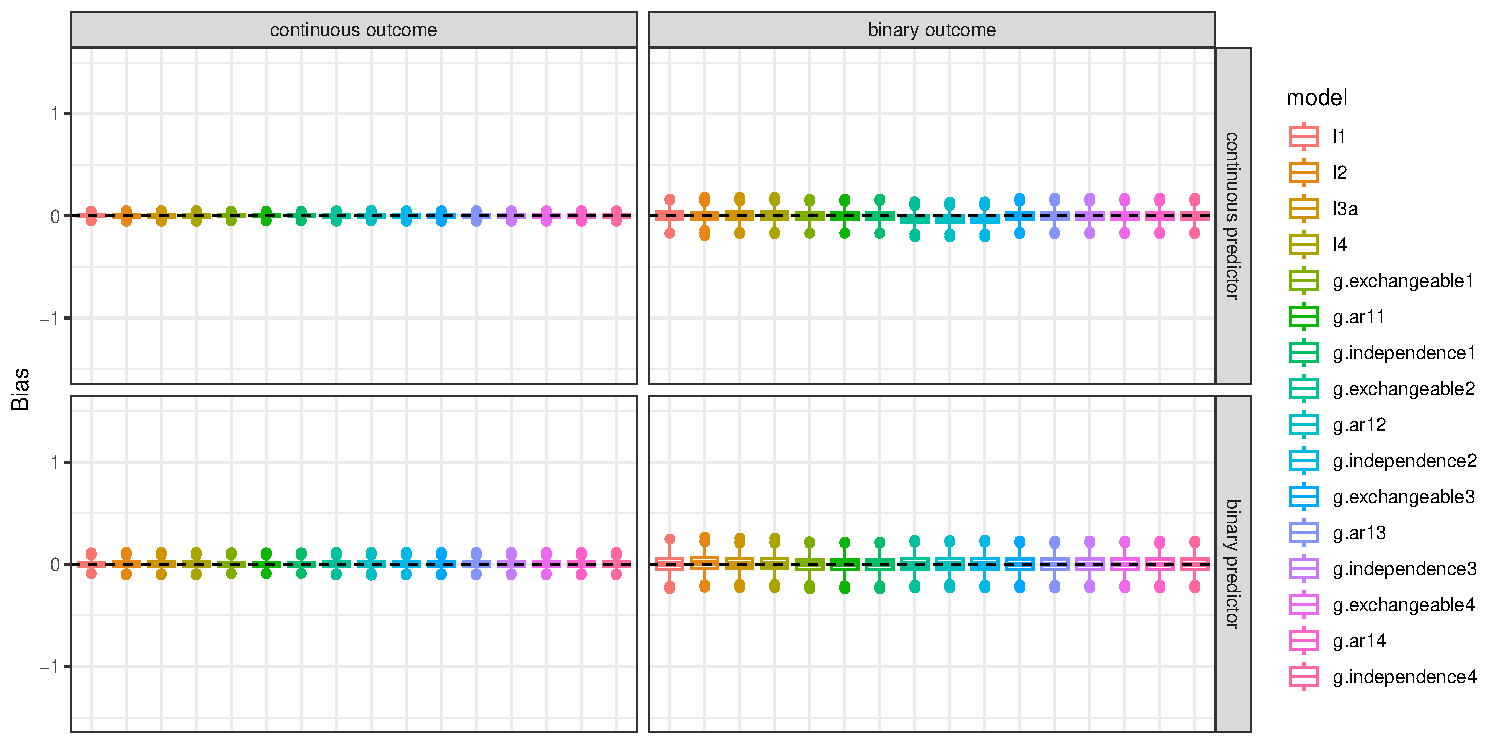
\includegraphics[width=\linewidth, keepaspectratio]{Figures/bias_plot_within_scenario01.pdf}
%     \label{fig:results-within-scenario01}
%     % \begin{figurenote}
%     %     \ldots
%     % \end{figurenote}
% \end{center}

% \begin{center}
%     \captionof{figure}{Bias in Within-Person Effect for Different Estimation Approaches (with $N = 200, T = 20, \sigma_{X,\text{b}} = 1, \sigma_u = 0, \gamma_{01} = 0$)}
%     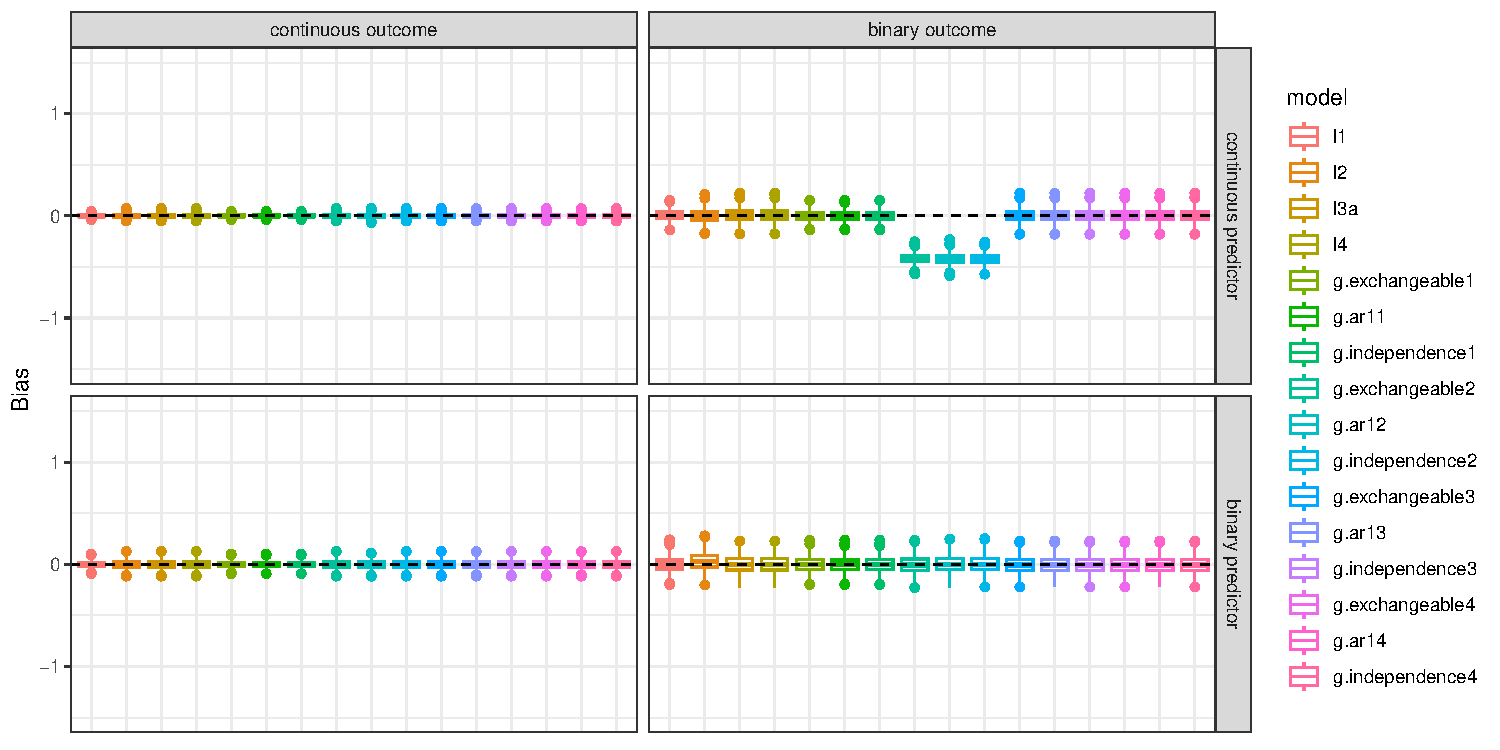
\includegraphics[width=\linewidth, keepaspectratio]{Figures/bias_plot_within_scenario02.pdf}
%     \label{fig:results-within-scenario02}
%     % \begin{figurenote}
%     %     \ldots
%     % \end{figurenote}
% \end{center}

% \begin{center}
%     \captionof{figure}{Bias in Contextual Effect for Different Estimation Approaches (with $N = 200, T = 20, \sigma_{X,\text{b}} = 0, \sigma_u = 0, \gamma_{01} = 0$)}
%     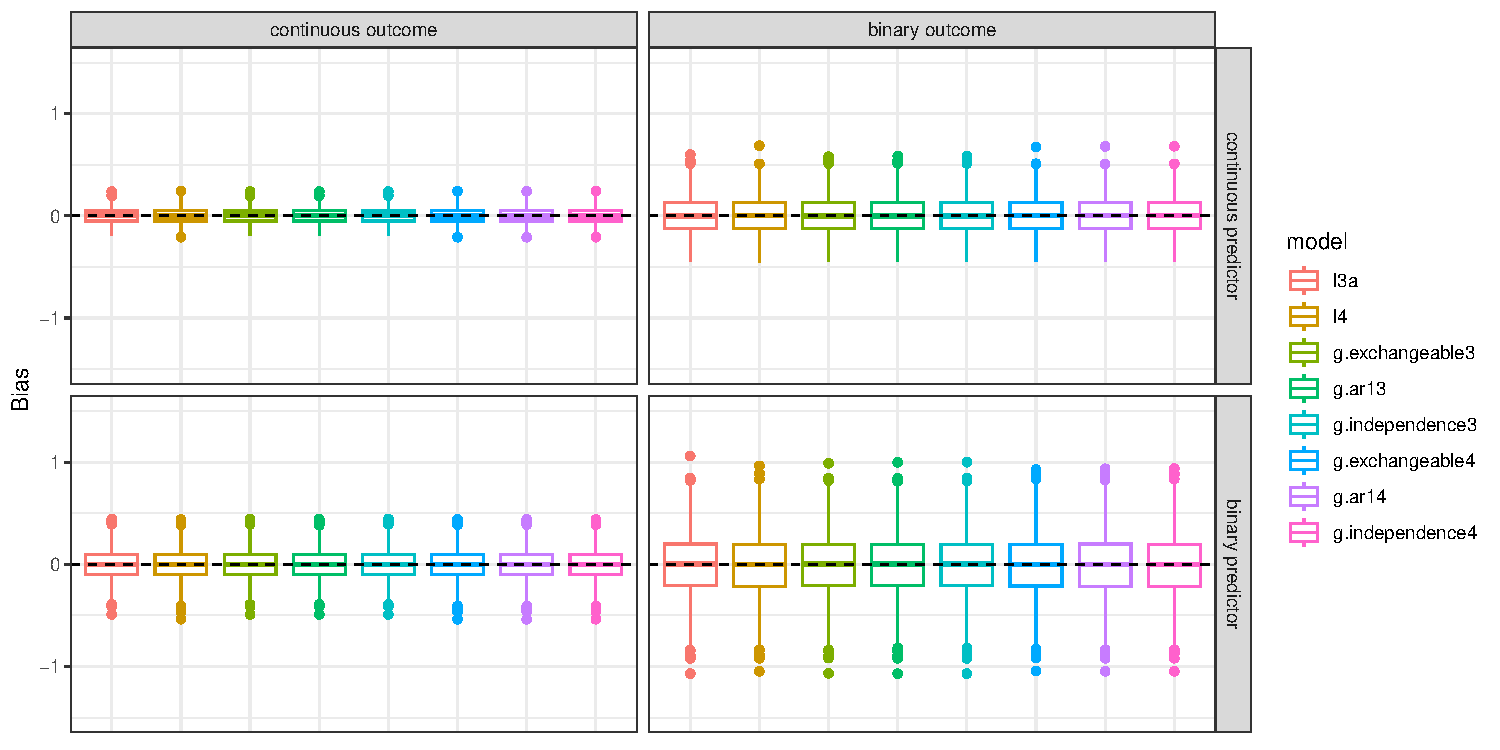
\includegraphics[width=\linewidth, keepaspectratio]{Figures/bias_plot_contextual_scenario01.pdf}
%     \label{fig:results-contextual-scenario01}
%     % \begin{figurenote}
%     %     \ldots
%     % \end{figurenote}
% \end{center}

% \begin{center}
%     \captionof{figure}{Bias in Contextual Effect for Different Estimation Approaches (with $N = 200, T = 20, \sigma_{X,\text{b}} = 1, \sigma_u = 0, \gamma_{01} = 0$)}
%     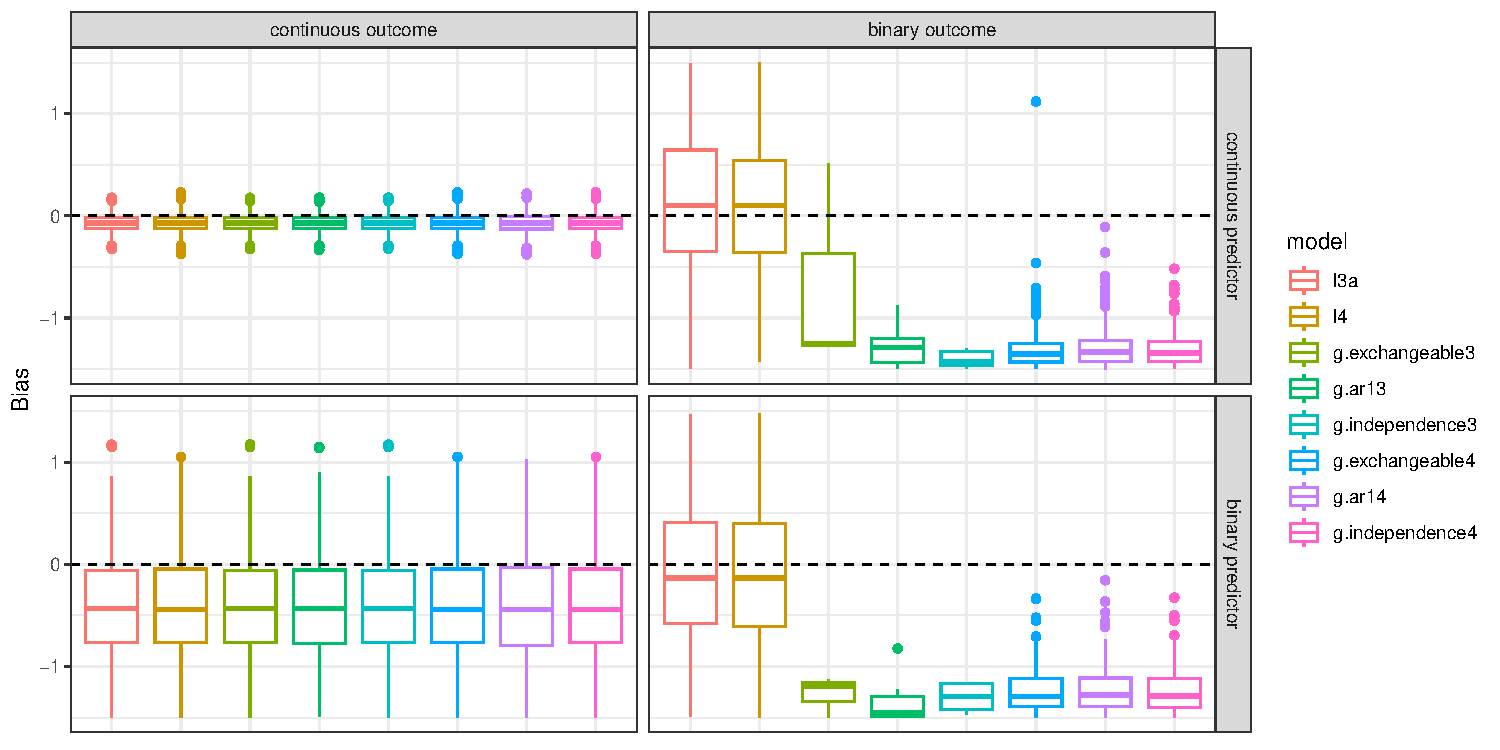
\includegraphics[width=\linewidth, keepaspectratio]{Figures/bias_plot_contextual_scenario2.pdf}
%     \label{fig:results-contextual-scenario02}
%     % \begin{figurenote}
%     %     \ldots
%     % \end{figurenote}
% \end{center}

% \input{Sections_revision1/Appendix1}
% \input{Sections_revision1/Appendix2}
% \input{Sections_revision1/Appendix3}
% \input{Sections_revision1/Appendix4}
% % \input{Sections_revision1/Appendix5}

% EXCERPTS FOR LATER USE

% \subsubsection{Continuous Predictor and Outcome}

% The model can be decomposed into a fixed and a random part. The fixed part, which remains constant across individuals, consists of the intercept \( \gamma_{00} \), the contextual slope \( \gamma_{01} \), and the within-person slope \( \beta_1 \). At first glance, it may not be obvious why the uncentered predictor represents the within-slope. As explained by \textcite{hoffman_longitudinal_2015}, this follows from the correlation between the cluster mean \( \mu_{X,i} \) and the raw predictor \( X_{it} \) (Equation~\ref{eqn:relationwithinmundlak}). Because these terms share variance in the outcome, their regression coefficients reflect only their unique contributions, making \( \beta_1 \) a within-person effect so that \( \beta_1 = \beta_\text{w} \) \parencite{mundlak_pooling_1978}.

% In the fixed part, \( \gamma_{00} \) represents the expected anxiety level for an individual whose cluster mean $\mu_{X,i}$ is zero, while \( \beta_1 \) quantifies how deviations from a person’s usual sleep duration (\(X_{\text{w},it} = X_{it} - \mu_{X,i}\)) relate to changes in their anxiety. The coefficient \( \gamma_{01} \) captures the degree to which the between-person effect---the association between a person’s typical sleep duration (\( \mu_{X,i} \)) and their overall anxiety level---differs from the within-person effect. Using the parameters $\beta_\text{w}$ and $\gamma_{01}$, we can directly compute the between-person effect as $\beta_\text{b} =\gamma_{01} + \beta_\text{w}$.

% The random part, which varies across individuals, consists of \( u_{0i} \), a normally distributed term with variance \( \sigma^2_{u0} \) that captures individual deviations from the average intercept \( \gamma_{00} \). Importantly, the model accounts for heterogeneity in these person-specific deviations both through the cluster mean of \( X \), which explains systematic differences, and through the random effect \( u_{0i} \), which captures unexplained individual variability.

% DISCUSSION

% \begin{enumerate}
%     \item Simulation results revealed that the effectiveness of disaggregation methods indeed depended on the estimation framework and on the variable type.
%     \item Simulation results revealed that, in the presence of contextual effects, the uncentered predictor method failed to consistently recover the within-person effect for GLMM, but also for the three GEEs with varying working correlation structures. It should be noted that the bias and variability in estimates of the uncentered method tended to be much greater for scenarios that involved binary variables compared to the familiar continuous predictor and outcome scenario. This implies that there is an even greater necessity of applying a disaggregation method in the binary case.
%     \item With a continuous outcome (DGMs 1 and 2), we found that all disaggregation methods (CWC, HB, MuCo) performed similarly across the GLMMs and the three GEEs. This suggests that with continuous outcome variables (i.e., in the MLM), we may be able to use the GEE for estimating the within-person and contextual effects.
%     \item However, in the presence of binary outcomes (DGMs 3 and 4), all GEEs implementations failed to consistently retrieve the within-person and contextual effects. Within the GLMM framework, Mundlak's contextual or the hybrid method was required to robustly retrieve the within-person effects. Unexpectedly, within GLMM the CWC method yielded biased results in a number of scenarios, which tended to be more substantial for a continuous predictor (vs. a binary one). 
% \end{enumerate}

% The simulation results demonstrated that the effectiveness of disaggregation methods depended on both the estimation framework and the variable type. In scenarios involving contextual effects, the uncentered predictor method failed to consistently recover the within-person effect, not only in the GLMM but also across all three GEE implementations, regardless of their working correlation structures. This issue was particularly pronounced in designs involving binary predictors or outcomes, where both bias and variability increased substantially, underscoring the greater necessity of applying proper disaggregation techniques in such cases. When the outcome was continuous (DGMs 1 and 2), all disaggregation methods (CWC, HB, MuCo) performed similarly across estimation frameworks, suggesting that GEE can be a viable alternative to GLMM for estimating within-person and contextual effects in linear models. In contrast, with binary outcomes (DGMs 3 and 4), none of the GEE variants consistently retrieved the disaggregated effects, while only the hybrid and Mundlak approaches performed robustly within the GLMM framework. Surprisingly, the CWC method yielded biased estimates in GLMMs under several conditions, particularly when the predictor was continuous. 

% The simulation results demonstrate that the effectiveness of disaggregation methods depends on both the estimation framework and the type of variables involved. As expected, when contextual effects were present, the uncentered predictor method failed to consistently recover the within-person effect, not only in the GLMM but also across all three GEE variants—regardless of their working correlation structure. This issue was particularly pronounced in scenarios with binary predictors or outcomes, where the bias and variability were considerably larger than in continuous-variable settings. These findings underscore the heightened importance of applying a proper disaggregation method, especially in models involving binary data. When outcomes were continuous (DGMs 1 and 2), the different disaggregation strategies (CWC, HB, MuCo) performed comparably well across all estimation approaches. This suggests that in such settings, GEEs may serve as a viable alternative to GLMMs for estimating both within-person and contextual effects. However, this equivalence breaks down in the binary case (DGMs 3 and 4), where none of the GEE approaches yielded accurate estimates. Instead, only the hybrid and Mundlak methods within the GLMM framework consistently recovered the within-person effects. Interestingly, the CWC method performed less reliably within GLMM when outcomes were binary, and this bias was most pronounced when the predictor was continuous. 


% Our simulations showed that for binary outcomes, the same cannot be said, as GEEs with a disaggregration method consistently failed to recover the effects, where the bias increased as a function of the random intercept variance. Again, this is expected as the non-linear logistic link results in a discrepancy between GLMM and GEEs coefficients \parencite[]{neuhaus_comparison_1991}. This divergence is known to increase with a greater random intercept variance, since the random intercept functions as an unobserved predictor, which is modelled in GLMM but not explicitly modeled in GEEs \parencite[(For an illustration of this, see \href{https://wardeiling.shinyapps.io/GLMM_population-averaged-and-person-specific-interpretations/}{wardeiling.shinyapps.io/GLMM\_population-averaged-and-person-specific-interpretations};)][]{neuhaus_comparison_1991, zeger_models_1988}. Specifically, this results in coefficients attenuated towards zero, as reflected in the GEEs with disaggregation methods, which were consistently fell below the zero-bias line, implying with positive true effects that they are smaller values.

% Specifically, under a logit link, GEE-based population-averaged estimates are attenuated toward zero to the extent that relevant predictors are omitted—leading to underestimation of within-cluster associations


% This divergence increases with greater random intercept variance, since the random intercept functions as an unobserved predictor (For an illustration of this, see \href{https://wardeiling.shinyapps.io/GLMM_population-averaged-and-person-specific-interpretations/}{wardeiling.shinyapps.io/GLMM\_population-averaged-and-person-specific-interpretations}). GLMM coefficients are statistically corrected for this unobserved heterogeneity, whereas GEEs coefficients are not \parencite[]{neuhaus_comparison_1991, zeger_models_1988}. As a result, under a logit link, population-averaged estimates are attenuated toward zero to the extent that relevant predictors are omitted—leading to underestimation of within-cluster associations, as reflected in our GEEs results, which consistently fell below the zero-bias line. 

% First, although the person-mean centered only approach (Method CWC) is often regarded as the default or “gold standard” for estimating within-person effects in the MLM literature \parencite[e.g.,][]{hamaker_fixed_2020, enders_centering_2007, raudenbush_adaptive_2009}, our results indicate that this strategy may be inadequate—and lead to biased estimates—in scenarios with binary outcomes. This is alarming as researchers who have been recommended this method for continuous outcomes, may be prone to transfer this habit to multilevel models with binary outcomes. To avoid bias, it is important that researchers insert the cluster mean of the predictor as predictor of the random intercept, as is done in Mundlak's contextual and the hybrid method. This rather intriguing finding may reflect differences in properties of the identity and the link function. Namely, \textcite[]{neuhaus_geometric_1993} show that omitting predictors that influence a binary outcome can seriously bias the regression coefficients, even if the omitted variable is independent of the included predictors (p. 807). In the formulation of method CWC, the person-mean of the predictor is omitted.


% Third, our findings shed light on some limitations of estimation with sample means within the GLMM. Across most scenarios, the simulations showed at least small bias in the estimates of the contextual effects. While several factors may contribute to this bias, it may be partially explained by Lüdtke’s bias, where the observed person-mean used for disaggregation is known to be an imprecise estimate of the true latent mean \parencite{ludtke_multilevel_2008}. In line with earlier work on using sample means for disaggregation methods \parencite{asparouhov_latent_2019}, we found that bias increased with stronger contextual effects, lower between-person variance, and fewer observations per person. Furthermore, we also found that overall bias in the contextual effect was much greater for binary (DGMs 2 and 4) as opposed to continuous predictors (DGMs 1 and 3). It is important to clarify that not all of this bias may be explained by Ludtke's bias and that there are likely other sources at play, some of which discussed earlier in when discussing practical challenges of binary predictors in the MLM context. To mitigate the bias introduced by using the observed mean, we recommend employing the more robust latent mean centering methods, in particular under binary predictors.

% Third, GLMMs were not exempt from bias in contextual effect estimates, particularly when the number of time points was small. This can be explained by Lüdtke’s bias, where the observed person-mean used for disaggregation is an imprecise estimate of the true latent mean \parencite{ludtke_multilevel_2008}. The bias is known to increase with stronger contextual effects, lower between-person variance, and fewer observations per person \parencite{asparouhov_latent_2019}, which we also found in the simulation study. Although latent mean centering methods are more robust, they are not yet widely implemented in standard GLMM software, which limits their practical use. As a result, we chose to utilize a more common implementation (the \texttt{lme4} package in R) without this functionality.


% Finally, unexpectedly we also found, despite claims about the robustness of GEEs against misspecification of the working correlation structure \parencite[e.g.,][]{zeger_models_1988, ballinger_using_2004}, extreme values in a substantial number of scenarios, in particular for the AR(1) structure with binary outcomes (see Appendix). However, AR(1) was not the correct structure in the underlying DGM and this only occurred when a disaggregation method was applied, which is not common practice within the GEEs literature. 

% \begin{enumerate}
%     \item All assumptions were met, future research should investigate robustness and investigate how both frameworks perform under these circumstances.
%     \begin{enumerate}
%         \item researchers using these methods may want to estimate both models, and report and attempt to explain any discrepant results \parencite[]{landerman_modeling_2011}.
%         \item Crucially, however, by avoiding random effects, GEEs circumvents some of the unverifiable assumptions required by GLMMs—such as the correct specification of the random effects distribution—which, if violated, can seriously bias estimates \parencite[]{hubbard_gee_2010}. 
%     \end{enumerate}
%     \item Moreover, we restricted our focus to models without random slopes for simplicity. Given that random slope models can be seen as one of the key advantages of the multilevel framework \parencite[]{bell_explaining_2015}, it is important to explore whether the present findings generalize to such cases.
%     \item Finally, our DGMs were limited to binary predictors and outcomes. Although prior work has explored multi-categorical predictors \parencite[e.g.,][]{yaremych_centering_2023},  extensions to multi-categorical outcomes remain an important direction for future research.
% \end{enumerate}

% This study has several limitations. 

% First, our simulations evaluated how well the within-person effect is recovered under DGMs that satisfy GLMM's and GEEs assumptions \parencite[For an overview, see][]{mcneish_unnecessary_2017}. However, these assumptions may be violated in practice, which can seriously bias estimates. In biomedical research, GEEs are often considered a safer alternative to random effects models, as some unverifiable random effects assumptions are omitted \parencite[]{hubbard_gee_2010}. Future research should investigate how both frameworks perform when these assumptions are violated, particularly whether the equivalence between GEE and GLMM always holds for continuous outcomes or that one framework will outperform the other.

% Second, given that random slope models can be seen as one of the key advantages of the multilevel framework \parencite[]{bell_explaining_2015} over the GEE framework that ignores this random slope heterogeneity, it is important to extend the DGMs to include a random slope and explore whether GEEs using dissaggregation are still able to retrieve the within-person effect  under a continuous outcome with random slope.

% Third, our DGMs were limited to binary predictors and outcomes. Although prior work has explored multi-categorical predictors \parencite[e.g.,][]{yaremych_centering_2023},  extensions to multi-categorical outcomes remain an important direction for future research.

\end{document}
